%% LyX 2.3.6.1 created this file.  For more info, see http://www.lyx.org/.
%% Do not edit unless you really know what you are doing.
\documentclass[12pt,twoside,american]{scrartcl}
\usepackage[T1]{fontenc}
\usepackage{geometry}
\geometry{verbose,tmargin=2cm,bmargin=2cm,lmargin=2cm,rmargin=1cm,footskip=1cm}
\pagestyle{headings}
\setlength{\parindent}{0cm}
\usepackage{color}
\usepackage{babel}
\usepackage{array}
\usepackage{float}
\usepackage{url}
\usepackage{graphicx}
\usepackage{tablefootnote}
\usepackage[unicode=true,
 bookmarks=true,bookmarksnumbered=true,bookmarksopen=false,
 breaklinks=true,pdfborder={0 0 1},backref=false,colorlinks=true]
 {hyperref}
\hypersetup{pdftitle={Internal Secrets of Infocom Games},
 pdfauthor={Michael Ko},
 pdfsubject={Everything you wanted to know about the internal working of all text-based Infocom games},
 pdfkeywords={Infocom,ZIL},
 pdfnewwindow=true,pdfstartview=XYZ,plainpages=false,colorlinks=true,linkcolor=black,citecolor=black,pdfpagelabels}

\makeatletter

%%%%%%%%%%%%%%%%%%%%%%%%%%%%%% LyX specific LaTeX commands.
\newcommand{\noun}[1]{\textsc{#1}}
%% Because html converters don't know tabularnewline
\providecommand{\tabularnewline}{\\}

%%%%%%%%%%%%%%%%%%%%%%%%%%%%%% User specified LaTeX commands.
\usepackage[T1]{fontenc}

\makeatother

\usepackage{listings}
\renewcommand{\lstlistingname}{Listing}

\begin{document}
\author{Michael Ko}
\title{Internal Secrets of Infocom Games\thanks{\protect\url{https://ifsecrets.blogspot.com} and \protect\url{https://docs.google.com/document/d/1yNa4M2gN5cG6WoKOSrHtS4_Sp4uwHt1Q7Pvtw8O8hFQ} }}
\subtitle{Everything you wanted to know about the internal working of all text-based
Infocom games}
\date{{[}2022-09-18{]}}

\maketitle
\pagebreak\tableofcontents{}

\section*{\vfill{}
\protect\pagebreak}

\section*{Introduction}

Decades ago, Infocom was synonymous with good storytelling and creative
puzzles. It wasn\textquoteright t the first company to release a text
interactive fiction game, but its first release, Zork I, made it the
flagbearer for all other IF games to follow. Infocom took over the
personal computer market for interactive fiction games by having their
games programmed in ZIL (Zork Implementation Language) which is a
compact language that easily handled text and object structures. ZIL
programs were compiled into Z-code, an assembly code that would run
on a \textquotedblleft Z-machine\textquotedblright . Infocom created
multiple Z-machine emulators (AKA Zork Interpreter Program or ZIP)
to run on various computers especially home computers like the TSR-80,
Apple II, and Commodore 64. Such an approach allowed a single program
to be run on different computers without having to create a separate
program for each machine.

Buried in these ZIL programs were the basic structure of how an Infocom
game is organized and executed. And it was Infocom\textquoteright s
parser which could understand complex commands with such a small amount
of code that seemed miraculous to IF fans. The inner workings of Infocom
games remained a mystery until reverse engineering was done that decoded
the Z-code format. Much of the knowledge about Z-code was documented
in the Z-Machine Standards Document by Graham Nelson and Mark Howell.
In this, the Z-code instructions and data structure used by some of
those instructions (like Vocabulary by \texttt{read} or objects by
\texttt{get\_prop}) tables were described. As it was a general document,
other data structures specific to Infocom games like verb syntaxes
were not mentioned. Several excellent utilities (infodump by Mark
Howell and ZILF by Jesse McGrew and Josh Lawren) have helped provide
more insight on the data structures of Infocom games. Utilities to
translate the Z-code to a more easily readable format did help show
the inner routines of the games. Without variable names, attribute
references, and object property names, making sense of the game code
remained difficult. An internal Infocom use only document, \textquotedblleft \emph{Learning
ZIL - or - Everything You Always Wanted to Know About Writing Interactive
Fiction But Couldn't Find Anyone Still Working Here to Ask}\textquotedblright ,
gave basic details about the how the games run and how the syntax
parts of the game were designed in ZIL. The release of an MDL-based
Zork source code did offer more insight into the inner workings of
the original Zork game, but understanding MDL was an added barrier.
While there are basic parsing and command processing algorithms in
the MDL-version of Zork, they were significantly changed when translated
to the microcomputer versions. The release of the \textbf{Mini-Zork}
source code and other tidbits from the Infocom cabinet helped unmask
and clarify the game code and the coding process that are essential
to all Infocom games.

This blog will describe those hidden details of Infocom games, using
\textbf{Zork 1} as the base. It will also provide some of the modifications
made to these core routines by specific Infocom games. Subsequent
post will provide the inner puzzle workings in all Infocom games.
Only the text games will be used. None of the graphics based games
are analyzed.

All routine and variable names in the Infocom source code (\textbf{Mini-Zork})
and documentation are in all capital letters. Game names are in bold.
Unnamed variables and routines are given names that are a best guess.

Apologizes for any errors in these posts. They'll be fixed if possible.

\section{ZIL, ZILCH, ZAP, and ZIP}

\subsection{Introduction}

ZIL is a derivative of MDL (MIT Design Language), a LISP-like language,
with a minimal set of instructions needed to created IF games. The
Infocom game files created from ZIL source code were run through the
ZIL compiler (ZILCH) to create Z assembly language code. This assembly
code was then sent through the Z Assembler Program (ZAP) to create
the actual Z-code. No copies of ZILCH or ZAP software have ever been
released or leaked to the public. There is also very little documentation
about these programs. The Infocom Cabinet files only mentions some
compilation flags used in ZILCH and the basic function of ZAP. The
final Z-code could be run on a \textquotedblleft Z-machine\textquotedblright{}
or any computer that emulated one using a Zork Interpreter Program
(ZIP). Different ZIP versions have different memory and processing
requirements. All have frequently used and writable data in their
\textquotedblleft core\textquotedblright{} memory which enables quicker
execution of the program. Less used and read-only data is read from
a storage medium (file or disk) on an as needed basis.

Throughout the history of Infocom, six versions of the Z-code were
recreated, but only the first 5 were used for text-only games.

\subsection{ZIP versions 1}

Many of the Z-code instructions used in Infocom games are in this
first version of ZIP. It is unclear what the memory requirements are
for it though. Only one ZIP 1 game, \textbf{Zork 1}, was ever released
by Infocom.

\subsection{ZIP version 2 }

ZIP 2 was used to create \textbf{Zork 1}-R15 and the first version
of Zork 2. It introduced frequent words (AKA abbreviations) and a
new header element (serial number) which is just a 6 digit ASCII representation
of the release date in year-month-day format. 

\subsection{ZIP version 3}

Version 3 was used to create a majority of the Infocom games. Infocom
documents indicates the version 3 compatible ZIP should have a minimum
of 40K (maybe 32K) of core memory and a floppy drive with at least
80K of storage. Due to limitations to the ZIP 3 format, the maximum
size game file is 128K. Also the response time should be a few seconds
for the average command. 

Deadline would be the first new game using this version. This version
increased the number of abbreviations and added more output functions.
Even after ZIP 4 and 5 were introduced, Infocom would produce 24 games
using ZIP 3.

For outputs, ZIP 3 compatible programs had 2 or 3 \textquotedblleft windows\textquotedblright{}
where text could be displayed instead of 1 in ZIP 1 and 2. One of
these, the status bar is not usually used unless a special flag bit
is set in the header. Most games create the status bar in the main
or lower, window(0). Two additional output streams were created. One
\textquotedblleft streams\textquotedblright{} the text into a specified
memory block. The other was called a command script which recorded
the input and output of the game.

Finally, game verification was added by adding a file length and checksum
into the header. The VERIFY command would check the game data file
against these values.

\subsection{Enhanced ZIP (EZIP), version 4}

Version 4, renamed Enhanced ZIP (EZIP), was introduced with \textbf{A
Mind Forever Voyaging}. A smaller version of EZIP was apparently created
called, LZIP, or lower-case EZIP for computers with memory limitations.
The minimal hardware requirements for EZIP were at least 128KB of
memory and a single disk drive that can at least access 140KB. The
computer system needs to have upper and lower case characters and
a screen to display 80 characters across with at least 14 lines. These
requirements would allow games to only take a few seconds to complete
a typical \textquotedblleft go\textquotedblright{} command. The maximum
size game file is 256K.

EZIP increased the memory space to allow more objects and rooms along
with longer words (up to 9 characters) in the vocabulary. Several
new Z-code operands also simplified some of the table-related coding
for these games, offered more ways to call routines, and gave more
control to how text displayed on the screen by dividing it up into
various windows.

The specs of EZIP limited these games to an IBM PC, Macintosh, enhanced
Apple //e, C128, Amiga, and Atari ST. Four games were released using
this. No known LZIP version of games seem to exist.

\subsection{Extended ZIP (XZIP), version 5}

Introduced with Beyond Zork, version 5 (XZIP) allowed for games with
more objects and rooms and added more opcodes for routine calling,
text, and table manipulations. Borderzone and Sherlock would be the
only other new games to use this version. Infocom would release its
Solid Goal (AKA Greatest Hits) series which were re-releases of past
popular games but in the XZIP compatible format. However these games
did not utilize the added functionality of XZIP.

\subsection{YZIP, version 6}

YZIP (successor to XZIP) is version 6 which mainly added mouse, graphical
windows, and menu functions with Z-codes. The graphical based Infocom
games used this version and will not be discussed.

\section{General structure of Infocom Games and Data Structures }

\subsection{Introduction and Story Headers}

Since version 1 of ZIP, the story header is a fixed 64 bytes at the
start of every Infocom game that provides information regarding the
location of specific data and code. The header for ZIP 1 games used
the first 9 words/18 bytes. Subsequent ZIP versions would add more
values into the header. XZIP (Version 5) would use all 32 words (64
bytes).

The original story header information about the game and addresses
to specific types of data. Details are in Appendix A. The first word,
ZVERSION, ensures that the ZIP is compatible with the given story
file and emulates the proper Z-machine version. The version number
is located in the first byte. The second byte has the mode flags which
are set by the ZAP assembler (for bits 0 and 1) and the ZIP at startup
for the remaining bits. START address will be the first operation
to be executed by the ZIP. It points to the first instruction and
not the start of the routine. The next three addresses are used by
the various instructions. All the object-related operators use the
address in OBJECT to manipulate the object data. The READ instruction
uses the Vocabulary data at VOCAB to match and tokenize the characters
in the input buffer. GLOBALS points to the table holding the global
variables data.

ZIP 1 Story Header: 

\begin{table}
\begin{tabular}{|l|l|l|}
\hline 
Word & Name & Function\tabularnewline
\hline 
\hline 
00 & ZVERSION & %
\begin{tabular}{l}
Byte 0: Z-machine version \tabularnewline
Byte 1: Z-machine mode\tabularnewline
\end{tabular}\tabularnewline
\hline 
01 & ZORKID & Release number\tabularnewline
\hline 
02 & ENDLOD & End address of pre-loaded memory, start of variable (or exchangeable
memory)\tabularnewline
\hline 
03 & START  & Address of first instruction (not routine), Program Counter\tabularnewline
\hline 
04 & VOCAB & Address to Vocabulary table\tabularnewline
\hline 
05 & OBJECT & Address to Object data\tabularnewline
\hline 
06 & GLOBALS & Address to Global Variable table\tabularnewline
\hline 
07 & PURBOT & Start address of read-only (static) memory\tabularnewline
\hline 
\end{tabular}

\caption{ZIP 1 Story Header}
\end{table}

Other information would be added to the story header with newer ZIP
versions. The complete layout is in Appendix A.

\subsection{The Memory Layout of Infocom Games }

The layout of data in the Infocom game files is fairly consistent
between games. An example using \textbf{Zork 1} is shown below. The
\textquotedblleft memory\textquotedblright{} of the emulated Z-machine
is first loaded with the header information starting at \$0000. Memory
from \$0000 up to PURBOT encompasses the writeable memory such as
variables, objects, tables, and buffers. Data after PURBOT is read-only
data such as syntax data, routines, preposition data, and strings.
The exact locations of the syntax data, action routines, and preposition
table are stored in global variables, not the header. The ZIP will
continue to load data into memory. All data up to the address in ENDLOD
must be loaded. The ZIP may decide to load data past ENDLOD at its
discretion. All data after ENDLOD can be swapped out with other disk-based
data as needed. Usually routines and strings are the data that is
swapped. All important and quickly accessible data remains resident
in memory below the ENDLOD address. A sample layout of data structure
in \textbf{Zork 1} gives more details (using infodump):
\begin{verbatim}
Base   End  Size
 0000    3F   40 Story file header
 0040    7D   3D Objects - Property Defaults (Address at OBJECTS, word 5)
 007E   974  935 Objects - Entries
 0975  203A 16C6 Objects - Property data
 203B  221A  1E0 Global Variables (Address at GLOBALS, word 6)
 221B  2C28  A0E Misc Data (such as tables and buffers)
 2C29  2CFE   D6 Syntax - Pointer table (Address at PURBOT)
 2CFF  33d4  6D6 Syntax - Entries (referred by the Pointer Table)
 33D5  34b6   E2 Action routine table (Address in global variables)
 34B7  3598   E2 Pre-action routine table (Address in global variables)
 3599  35DE   46 Preposition table (Address in global variables)
 35DF  46CA 10EC Vocabulary (Address at VOCAB, word 4)
 46CC  EDC5 A6FA Routines (Load up to ENDLOD, $5DEC here)
 EDC6 14328 5563 Strings
14329 143FF   D7 Empty (fill up to the end of memory page)
\end{verbatim}

\subsection{The Massive Object Table}

Objects are the heart of the Infocom games and are the first data
after the story header. Storing them in a logical and efficient manner
for the game to access is important. Each object contains information
such as the name, properties and attributes. It will also have a parent
and possibly siblings. The object\textquoteright s parent is usually
a room or container that contains the object. Siblings are objects
that are in the same room or container. Rooms are also considered
objects and have a generic ROOMS object as the parent for all rooms.
Attributes are true/false bits that set various characteristics of
an object such as is it takable (TAKEBIT) or a source of fire (FLAMEBIT).
They are numbered 0 to 31. Each object will define all the attributes.
Properties are like attributes but hold groups of bytes instead of
a bit. The maximum size for a property is 8 bytes. If no property
is given for an object, the default property value (a word) is used.
Properties are numbered 1 to 31. Objects are numbered from 1 to 255.

\newpage{}
\begin{itemize}
\item Default Property Table: 
\begin{itemize}
\item 31 words that are the default property values if it is not explicit
set for a specific object
\end{itemize}
\item Object Entries - repeated for all objects
\begin{itemize}
\item 4 bytes representing the 32 attribute bits (\#0=top bit of byte 0,
\#31=bottom bit of byte 3) 
\item 1 byte each for object number of the parent, sibling, and child of
the object 
\item 1 word address to that object\textquoteright s property table 
\end{itemize}
\item Property Table - repeated for all objects with their own property
table 
\begin{itemize}
\item 1 byte for size of the object name in words 
\item Z-string of the object name 
\item 1 byte for property info (LLLNNNNN) 
\begin{itemize}
\item bits 5-7 = length of property-1 (length 1-8 bytes is represented as
0-7) 
\item bits 0-4 = property number 
\end{itemize}
\item 1-8 bytes of property data 
\item The 1 byte property info and 1-8 property data are repeated for each
property, listed in descending order
\end{itemize}
\end{itemize}
Example object property table:

\begin{figure}[H]

\includegraphics[width=1\textwidth]{figures/PropertyTableExample}

\caption{Property Table Example}
\end{figure}

The meaning of an attribute or property number is consistent in all
objects in that game but not consistent between games. For example,
the attribute bit and properties used in \textbf{Zork 1} are listed
in Appendices B and C. The number of objects is not specifically stored
here but calculated based upon the number of object entries. It can
also be calculated by the difference between the addresses of the
first object entry and first property table entry divided by 9 bytes
for each entry.

\subsection{Global Variables}

The section following the objects is a 480 byte block corresponding
to 240 global variables with each holding a word. By default in Infocom
version 1-3 games, variable 0 contains the object number of the player\textquoteright s
current location. Variable 1 is the score while variable 2 is the
number of turns or game time. A game does not need to use all 240
global variables and can use part of this memory block for other variable
data such as tables and buffers. The addresses to these other data
structures as well as addresses to specialized grammar structures
like syntax entries, preposition table, and action routine table are
typically stored in global variables.

\subsection{Tables and Buffers}

Between the last global variable and the start of the static data
(at PURBOT), there is usually extra memory that is used to store custom
data structures. These are typical tables and buffers. Tables are
a fixed set of words where the first word (element 0) contains the
number of elements in the table. Examples include tables to hold the
direct or indirect object numbers. A buffer is just a fixed set of
bytes used to hold any type of data. The most common buffers used
in Infocom games are the input buffer (INBUF) or token buffer (LEXV).
These data structures are not standard to ZIL and are specific to
Infocom games. For ZIP 1-3 games, these tables are located in the
preloaded memory of the computer. For EZIP and XZIP games, tables
can also be located amongst the game routines. The addresses to these
buffers and tables are usually stored in specific global variables
but can sometimes be hardcoded into the routines that use them. If
a game does not need all 240 global variables, the space for those
unused variables can be used for buffers and tables. Infocom games
have their own custom ZIL routines for reading and writing to these
structures. 

\subsection{Vocabulary}

The vocabulary contains information about every valid word in the
game. It begins with a header which contains the information about
separator characters and the entries themselves.
\begin{itemize}
\item 1 byte - N number of separator characters (used to mark the end of
words)
\item N bytes - list of N separator characters
\item 1 byte - length of each vocabulary entry (Z-string + word type data)
\begin{itemize}
\item ZIP 1-3 games: 4 bytes for Z-string
\item EZIP and XZIP games: 6 bytes for Z-string
\item All games use 3 bytes for the word type data except Sherlock (uses
2 bytes)
\end{itemize}
\item 2 bytes - number of vocabulary entries
\end{itemize}
A long list of vocabulary entries will follow this header. Each entry
starts with a 4 or 6 byte Z-string of the word. The remaining 2 or
3 bytes contain:
\begin{itemize}
\item 1 byte for word type:
\end{itemize}
\medskip{}

\begin{tabular}{|>{\centering}p{0.1\columnwidth}|>{\centering}p{0.1\columnwidth}|>{\centering}p{0.1\columnwidth}|>{\centering}p{0.1\columnwidth}|>{\centering}p{0.1\columnwidth}|>{\centering}p{0.1\columnwidth}|>{\centering}p{0.1\columnwidth}|>{\centering}p{0.1\columnwidth}|}
\hline 
\multicolumn{6}{|c|}{Primary word type} & \multicolumn{2}{c|}{Secondary word type}\tabularnewline
\hline 
Bit 7 & Bit 6 & Bit 5 & Bit 4 & Bit 3 & Bit 2 & Bit 1 & Bit 0\tabularnewline
\hline 
\$80 & \$40 & \$20 & \$10 & \$08 & \$04 & \$00 = Noun & \$02 = Adjective\tabularnewline
\hline 
Noun & Verb & Adjective & Direction & Preposition & Special & \$01 = Verb & \$03 = Direction\tabularnewline
\hline 
\end{tabular}

\medskip{}

\begin{itemize}
\item 1 byte for second ID value - The secondary ID value if a secondary/non-default
word type is requested (original format, all games except \textbf{Sherlock}) 
\item 1 byte for default ID value - The default ID value 
\end{itemize}
ID values are a special number that corresponds to the token such
as a verb number for a verb. For example, the default ID value for
a the noun \textquotedblleft MATCH\textquotedblright{} would be its
object number. During word type matching, the default value is returned
if there is a match.

If a secondary word type is also given and is a valid word type, then
the secondary ID value is given. If there is no match, then the default
one is returned. For example, \textquotedblleft INFLAT\textquotedblright{}
has its last 3 bytes as {[}62 a8 d3{]}. Bits 7-2 of the word type
value \$60 indicate this token can be a verb (\$40) or adjective (\$20).
The last 2 bits (\$02 in this example) indicates the secondary word
type, adjective. So the default word type is a verb. When the program
checks if \textquotedblleft INFLAT\textquotedblright{} is a verb or
adjective:

\begin{lstlisting}[basicstyle={\ttfamily}]
call wt?("INFLAT",$40) or <WT? "INFLAT", PS?VERB>
call wt?("INFLAT",$20) or <WT? "INFLAT", PS?ADJECTIVE>
\end{lstlisting}

the word type matching routine will return the default, \$d3. If a
second word type (\$02) is also passed to the matching routine:

\begin{lstlisting}[basicstyle={\ttfamily}]
call wt?("INFLAT",$40,$02) or <WT? "INFLAT", PS?VERB, P1?ADJECTIVE>
call wt?("INFLAT",$20,$02) or <WT? "INFLAT", PS?ADJECTIVE, P1?ADJECTIVE>
\end{lstlisting}

then the routine will return \$a8. If the second word type does not
match, such as \$03 (for direction), then the default, \$d3, will
be returned.

The E/XZIP vocabulary introduced 6 bytes for the Z-string which allowed
for longer tokens (maximum of 9 characters). The size of each entry
in Vocabulary grew to 9 bytes. A newer compressed vocabulary entry
format was also created which used a single ID value. The need for
a second ID value mainly occurred with tokens that can be a direction
and preposition. This format only had 8 byte entries. Only \textbf{Sherlock}
used this compressed vocabulary format and had modified syntax routines
which used the PREP table to look for the this second ID value (preposition
value) in situations where a token could a direction or preposition.

\subsection{Strings}

Much of the code for Infocom games are the various descriptions and
text responses that are stored as strings in the special Z-character
format. It is a compressed format where the characters are represented
by 5 bits instead of 8. This allows 3 letters to be stored in the
space of 2 bytes instead of 3. More detailed information including
the character sets is in the Z-Machine Standards Document.

\section{Syntax Entries - The Biggest Mystery of them All}

\subsection{Introduction}

Probably the most innovative part of Infocom games were their ability
to understand commands written in conversational English. The different
types of grammar information were discussed in the \textquotedblleft Learning
ZIL\textquotedblright{} document. The structure of syntax entries
in ZIL was shown, but the layout in the Z-code files was not mentioned.
Infodump and ZILF do provide some extra information about the syntax
structure. There are 3 additional grammar-related data blocks in the
game not mentioned in the header: prepositions, syntax pointer table,
and syntax entries.

\subsection{Prepositions}

There is a separate table of prepositions to speed up the syntax matching
process.
\begin{itemize}
\item 1 byte for number of prepositions
\item 2 word entries: address of preposition in vocabulary and preposition
number
\end{itemize}
The prepositions are numbered from \$FF and decrease. The address
to this table is stored as a global variable. EZIP and XZIP use a
compact form of the Preposition table that used a byte instead of
a word for the preposition ID number.

\subsection{Syntax Entry Pointer Table}

The syntax entries are probably the most confusing part of Infocom
games thanks to the lack of documentation. They provide the syntax
structure for a particular action. To find the matching syntax entry,
the verb number is needed. Since verbs can have synonyms, different
verbs can have the same verb number like \textquotedblleft GET\textquotedblright{}
and \textquotedblleft TAKE\textquotedblright . So they would use the
same syntax entries. The syntax entry table lists the address where
the group of syntax entries for that specific verb number is located.
This table is just a block of addresses with verb number \$FF is the
first address. Subsequent addresses correspond to smaller verb numbers.

\subsection{Syntax Entries}

PARSER will then look through each of the syntax entries for the matched
verb number and return the entry that best completely matches the
given (if any) prepositions and noun clauses types. For example, the
syntax entry table for verb number \$F3 (or GET) has 7 different syntax
entries. The syntaxes of \textquotedblleft GET object\textquotedblright ,
\textquotedblleft GET object from object\textquotedblright , and \textquotedblleft GET
on object\textquotedblright{} would correspond to 3 different entries.
To store this grammatical information, this group of entries start
with a byte indicating how many entries for that verb. It is followed
by multiple 8 byte entries for all acceptable grammatical combinations:\medskip{}

\begin{tabular}{|l|l|}
\hline 
Byte & Contents\tabularnewline
\hline 
\hline 
0 & Number of object clauses\tabularnewline
\hline 
1 & Prep number for direct object\tabularnewline
\hline 
2 & Prep number for indirect object\tabularnewline
\hline 
3 & GWIMBIT number for direct object\tabularnewline
\hline 
4 & GWIMBIT number for indirect object\tabularnewline
\hline 
5 & LOC byte for direct object\tabularnewline
\hline 
6 & LOC byte for indirect object\tabularnewline
\hline 
7 & Action Number\tabularnewline
\hline 
\end{tabular}

\subsection{Get What I Mean (GWIM) Feature}

The GWIMBIT number is used in the FIND feature mentioned in section
9.5 of \textquotedblleft Learning ZIL\textquotedblright{} to find
unspecified but necessary objects in a command. PARSER will attempt
to find an object in the current location with a set attribute flag
corresponding to the GWIMBIT number. If only one object is found to
match, it will assume the user meant that object and use it in the
given command. If no object or more than one object matches, PARSER
will ask for clarification (called orphaning). The player can then
give a clarifying answer without retyping the entire previous command
or type a completely new command.

For example, the syntax entry for \textquotedblleft IGNITE OBJ WITH
OBJ\textquotedblright{} has a GWIMBIT number for the indirect object
set to the FLAME bit. If that entry is the best syntax match the command
\textquotedblleft IGNITE TORCH\textquotedblright , the indirect object
is still missing. PARSER will try to find an object with the FLAME
bit set to use as the indirect object. If a an object in the current
location has the FLAME bit set (like a lantern), PARSER will assume
the indirect object is the lantern. The command will then assume to
be \textquotedblleft IGNITE TORCH WITH LANTERN\textquotedblright{}
and the indirect object will be set to LANTERN.

\subsection{Location Restriction of Objects}

The LOC byte is probably the most mysterious value in the syntax entry.
The highest 7 bits indicate how PARSER searches and checks on requested
objects. For example, PARSER will not complete an action with an object
on the ground if its syntax entry requires an object be held or carried.
While \textquotedblleft Learning ZIL\textquotedblright{} has listed
9 possible properties, the source code for \textbf{Mini-Zork} indicates
only 7 are used through version 3:\medskip{}

\begin{tabular}{|>{\centering}p{0.1\columnwidth}|>{\centering}p{0.1\columnwidth}|>{\centering}p{0.1\columnwidth}|>{\centering}p{0.1\columnwidth}|>{\centering}p{0.1\columnwidth}|>{\centering}p{0.1\columnwidth}|>{\centering}p{0.1\columnwidth}|>{\centering}p{0.1\columnwidth}|}
\hline 
Bit 7 & Bit 6 & Bit 5 & Bit 4 & Bit 3 & Bit 2 & Bit 1 & Bit 0\tabularnewline
\hline 
\multicolumn{4}{|c|}{Location-related Flags} & \multicolumn{4}{c|}{Possession-related Flags}\tabularnewline
\hline 
\$80 & \$40 & \$20 & \$10 & \$08 & \$04 & \$02 & \$01\tabularnewline
\hline 
{\footnotesize{}HELD} & {\footnotesize{}CARRIED} & {\footnotesize{}ON-GROUND} & {\footnotesize{}IN-ROOM} & {\footnotesize{}TAKE} & {\footnotesize{}MANY} & {\footnotesize{}HAVE} & {\footnotesize{}Not used}\tabularnewline
\hline 
{\scriptsize{}At top level and not inside another container} & {\scriptsize{}Not at top level, contained inside another object} & {\scriptsize{}At top level of a room and not inside another container} & {\scriptsize{}Not at top level, contained inside another object on
the ground} & {\scriptsize{}Will automatically TAKE object in the current location
if necessary before using it} & {\scriptsize{}Multiple objects are allowed for a particular action} & {\scriptsize{}Must already be in the user\textquoteright s possession} & \tabularnewline
\hline 
\end{tabular}\medskip{}

When the GWIM feature tries to search for an unspecified objected,
that routine needs to know how far to search. This is indicated by
the flags for HELD, CARRIED, IN-ROOM, and ON-GROUND which guide how
the function, SEARCH-LIST, finds objects in the given location (a
room or the user). More details will be given in section 13.2.

\textquotedblleft Learning ZIL\textquotedblright{} does mention an
EVERYWHERE and ADJACENT option, but there is no evidence that they
were ever used in version 1-5 games as confirmed by the internal Infocom
documents on ZIL. It could\textquoteright ve been used in the graphical
YZIP- based games.

\subsection{Pre-actions and Actions}

The action number is used to look up the routine address from the
ACTION and PRE-ACTION tables. These tables sequentially list the packed
addresses with any reference table. All syntaxes that refer to a similar
action (INSERT DOWN object, DROP object, and SPILL object IN object)
will use the same action number. INSERT object ON object and INSERT
object UNDER object use two different action numbers as the game processes
these actions differently. The action number is also used to lookup
the address for the pre-action routine if one exists (if not, \$0000
is used). A pre-action routine can check the objects, variables, or
game status before a particular action routine is called. The same
pre-action routine can be used with different action routines.

\subsection{An Example}

Multiple verbs have the same verb number such as CARRY, GET, and TAKE
in this example. The verb number will then correspond a group of syntax
entries. Here only 3 are used:
\begin{verbatim}
[02 00 f0 11 00 64 00 39] "carry OBJ from OBJ"     
[01 f9 00 00 00 00 00 31] "carry out OBJ"     
[01 00 00 11 00 34 00 39] "carry OBJ"
\end{verbatim}
In the first example, the \$02, indicates two noun clauses required
for that syntax. The next two bytes indicate the required prepositions
for the noun clauses. The \$00 indicates no preposition before the
direct object clause. The \$F0 refers to the preposition for the indirect
object clause, FROM in this case. The GWIMBIT number \$11 is the attribute
to check on objects if the direct object is missing. There is no GWIMBIT
number for the indirect object. The direct object LOC byte \$64 indicates
the direct object should be CARRIED or ON-GROUND. Also, multiple objects
can be in the direct object clause. In the second example, the OUT
preposition is needed before the direct object. In the third example,
the direct object LOC byte \$34 indicates the direct object needs
to be ON-GROUND or IN-ROOM. The last value (\$39 or \$31) is the action
number which indicates what specific routine to execute for that command.
Since the first and third examples are very similar, the same routine
will be used for both types of commands.

\subsection{Update: Compact Syntaxes to Save Space}

A variable sized syntax entry format was used only with Sherlock to
help save space. There are 3 sizes for the syntax entries based upon
the number of noun clauses. The format is described below. The preposition
number is stored in the lower 6 bits (after subtracting \$C0/192 from
the preposition number) of bytes 0 and 3.\medskip{}

\begin{tabular}{|>{\raggedright}p{0.1\columnwidth}|>{\raggedright}p{0.2\columnwidth}|>{\raggedright}p{0.09\columnwidth}|>{\raggedright}p{0.09\columnwidth}|>{\raggedright}p{0.09\columnwidth}|>{\raggedright}p{0.09\columnwidth}|>{\raggedright}p{0.09\columnwidth}|>{\raggedright}p{0.09\columnwidth}|}
\hline 
 & Byte 0 & Byte 1 & Byte 2 & Byte 3 & Byte 4 & Byte 5 & Byte 6\tabularnewline
\hline 
No objects & \# of objects (high 2 bits) / Prep ID (low 6 bits) & Action Number & - - - & - - - & - - - & - - - & - - -\tabularnewline
\hline 
Only direct object & \# of objects (high 2 bits) / Prep ID (low 6 bits) & GWIMBIT byte & LOC byte & Action Number & - - - & - - - & - - -\tabularnewline
\hline 
Direct and indirect objects & \# of objects (high 2 bits) / Prep ID (low 6 bits) & GWIMBIT byte & LOC byte & Prep ID (low 6 bits) & GWIMBIT byte & LOC byte & Action Number\tabularnewline
\hline 
\end{tabular}

\section{Execution of Infocom Games - An Overview}

\subsection{Introduction}

For all of their perceived complexity, Infocom games have a fairly
straightforward and consistent method of getting player commands,
parsing them, and executing them quickly. Each game would start with
initial setting of global variables and interrupts. This loop starts
with PARSER getting a command. It will then check and extract all
needed grammatical information. The game will use PERFORM to call
an action on the various objects in that command. CLOCKER will check
and executed any interrupts if necessary. Finally, the program repeats
this indefinitely or the game stops. Each game used the same basic
code from initialization of the game through handling interrupts.
The repeated use of previous code help minimize new bugs and kept
the play of the games consistent. But every game had some kind of
new code which could introduce bugs. The description of these main
backbone routines will be from the original \textbf{Zork 1} game from
1979. Information about updates to these routines will then follow
each section.

\subsection{Initialization with GO}

Initialization of each game begins with the GO routine which performs
(at least) four required tasks:
\begin{itemize}
\item Set important game variables like object number for WINNER or starting
location
\item Set any interrupt routines
\item Display the version information of the game
\item Execute the LOOK command for the starting location
\end{itemize}
The game then moves to the MAIN-LOOP.

\subsection{Heart Beat of the Game with MAIN-LOOP}

The game will repeatedly get new commands and execute them in an indefinite
loop, the MAIN-LOOP. The commands are obtained and parsed using PARSER
which returns the action, direct objects, and indirect objects referenced
by the given command. This loop will then call PERFORM to execute
the given action on all the direct and indirect objects. The turn
of the loop will end by calling CLOCKER which executes any necessary
interrupts. MAIN-LOOP will then repeat all of these steps indefinitely.

\subsection{Understanding the User with PARSER}

PARSER takes the player\textquoteright s input or any remaining input
from the last command and extracts the parts of command: verb, direct
object, and indirect object. The part of speech of tokens are identified
and later used by CLAUSE to find the start and end of object clauses.

\subsection{Completing Previous Command with ORPHAN-MERGE}

If a previous command was orphaned, the given command is examined
to by ORPHAN-MERGE to see if it supplies the missing information from
the orphaned command. If so, then ORPHAN-MERGE combines the new information
with the previous command. PARSER continues to process this fixed
command just like any other command.

\subsection{Match the Command with SYNTAX-CHECK}

The use of syntax templates allowed Infocom games to understand multiple
commands using similar tokens but in different orders. After PARSER
identifies the verb, direct object, and indirect object, SYNTAX-CHECK
will try to match a syntax template to the given verb, prepositions,
and objects. The action with the matched syntax template is returned.
If the best matched syntax template still has missing objects, the
game will attempt to supply them with objects in the current location.

\subsection{Find the Objects with SNARF-OBJECT}

After the matching syntax template and objects are verified, the game
will process each object clause and match the objects with objects
from the game. It will also handle modifiers like EXCEPT and quantities
like ALL.

\subsection{Final check on Objects with TAKE-CHECK and MANY-CHECK}

The game will also confirm if the objects need to be taken first (TAKE-CHECK)
and if multiple objects are allowed for the action (MANY-CHECK). Once
all the checks are completed, the game creates a table of all the
objects that are referred in each object clause.

\subsection{Call the Actions with PERFORM}

Finally, the game will execute the requested action (PRSA) on the
given direct (PRSO) and indirect (PRSI) objects with PERFORM. If one
noun clause has one object but the other has multiple, the game will
cycle through the clause with the multiple objects and use the same
object for the other clause. However, if both clauses have multiple
objects, only the direct objects will be cycled. Only the first indirect
object will be used.

\subsection{Tick the CLOCKER}

After the player command(s) are performed, the game\textquoteright s
interrupt system \textquotedblleft ticks\textquotedblright . Any interrupt
whose tick count reaches 1 will have its associated routine called
and then become disabled.

\subsection{Graphic representation of Game Flow}

Routine layout for \textbf{Zork 1}. Dotted lines indicate the order
of function calls by MAIN-LOOP.

\begin{figure}[H]
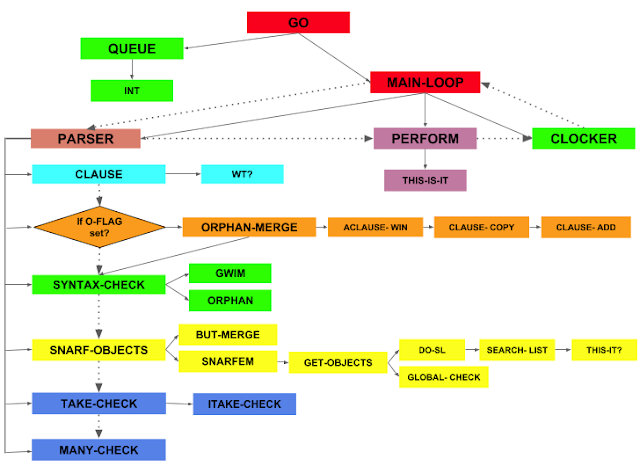
\includegraphics[width=1\columnwidth]{figures/RoutineLayoutForZork1}

\caption{Routine Layout for \textbf{Zork 1}}

\end{figure}


\section{GO - Gentlemen, Start Your Engines!}
\begin{description}
\item [{Arguments:}] None
\item [{Return:}] None
\end{description}

\subsection{Introduction}

Every Infocom game begins with an initialization routine, GO, that
sets certain variables and executes specific routines. It will then
jump into the MAIN-LOOP which will indefinitely ask for commands from
the user and process them.

\subsection{Running GO}

All Infocom games have the similar initialization routine for each
game. \textquotedblleft Learning ZIL\textquotedblright{} mentions
that the GO routine should:
\begin{itemize}
\item Set special global variables
\item Set interrupts, usually with the QUEUE or INT routines
\item Display an opening text/title screen
\item Call V-VERSION to show copyright information, release number, and
serial number
\item Call V-LOOK to describe the current location
\item Call the MAIN-LOOP
\end{itemize}
The important global variables that are set include WINNER (object
number for current active actor which is usually the PLAYER object),
HERE (current location of the WINNER), and LIT (indicates if the current
location is lit). All version 4 (except AMFV) and 5 games will also
check the width of the screen. Some games will not execute if the
screen width is too small. Infocom documentation recommends all games
start with an opening title screen and display game information before
showing the current locations description.

\section{MAIN-LOOP - Heart of the Game}
\begin{description}
\item [{Arguments:}] None
\item [{Return:}] None
\end{description}

\subsection{Introduction}

MAIN-LOOP is the heart of all Infocom games and keeps the game structure
orderly. It repeatedly requests for parsed commands and loops indefinitely.
MAIN-LOOP does not get modified too much with newer games. Many of
the changes were to make programming game-specific details and restrictions
easier to do. These game changes essentially provided more checks
on the player input and provided better responses. Only significant
changes to MAIN-LOOP will be later described.

\subsection{The Details}

MAIN-LOOP will call PARSER to ask and process a user\textquoteright s
command. If PARSER cannot properly parse the command, MAIN-LOOP will
continue to call PARSER to process new commands. If it has successfully
processed a command, PARSER will set PRSA (parser action) with the
requested action number (the 8th byte in a syntax entry) and fill
the PRSO (parser direct object) and PRSI (parser indirect object)
tables (P-PRSO and P-PRSI) with all the direct and indirect objects
requested. This is different to what is described in \textquotedblleft Learning
ZIL\textquotedblright . MAIN-LOOP then loops and acts upon all the
objects:
\begin{enumerate}
\item Check the number of objects in the direct and indirect clauses
\item If the direct objects clause has no objects, then see if the action
is GO.
\begin{enumerate}
\item If so, then call PERFORM with GO and the direction in PRSO.
\item If no objects are needed for the requested action, then call PERFORM
on PRSA with no objects
\item If at least 1 object clause is needed for the requested action, then
print an error message. Display a specific error message if the command
is an invalid response to an orphaned command.
\end{enumerate}
\item One clause will be designated the multiple one and one clause has
a constant object, first one in the clause.
\item Call the requested action with PERFORM multiple times for each object
in the multiple object clause as while the other clause just has its
first object used.
\begin{enumerate}
\item If M-END is returned, then halt the processing of multiple objects.
Erase any remaining commands.
\item If M-END is not returned, then continue looping through the multiple
objects
\end{enumerate}
\item Increase number of turns by 1 (even if multiple object are processed).
\item Call CLOCKER to check interrupts even if the given command was not
valid. This was later changed in Deadline and other future games to
only calling CLOCKER if PARSER was successful.
\end{enumerate}

\subsection{Details of Multiples of Multiples}

The MAIN-LOOP handles commands with multiple objects for a given action.
It will loop through these objects and execute the same action for
each object. However, there is some confusion as to how it determines
preference if two sets of objects are given. The examples below show
how MAIN-LOOP iterates through multiple objects.\medskip{}

\begin{tabular}{|>{\raggedright}p{0.3\textwidth}|>{\raggedright}p{0.3\textwidth}|>{\raggedright}p{0.3\textwidth}|}
\hline 
{\footnotesize{}Multiple Direct Objects} & {\footnotesize{}Multiple Indirect Objects} & {\footnotesize{}Multiple Direct and Indirect Objects}\tabularnewline
\hline 
\hline 
{\footnotesize{}IGNITE CANDLE AND PAPER WITH TORCH}{\footnotesize\par}

{\footnotesize{}\qquad{}IGNITE CANDLE WITH TORCH}{\footnotesize\par}

{\footnotesize{}\qquad{}IGNITE PAPER WITH TORCH} & {\footnotesize{}CUT TREE WITH AXE AND SWORD}{\footnotesize\par}

{\footnotesize{}\qquad{}CUT TREE WITH AXE}{\footnotesize\par}

{\footnotesize{}\qquad{}CUT TREE WITH SWORD} & {\footnotesize{}IGNITE CANDLE AND PAPER WITH TORCH AND FIRE}{\footnotesize\par}

{\footnotesize{}\qquad{}IGNITE CANDLE WITH TORCH}{\footnotesize\par}

{\footnotesize{}\qquad{}IGNITE PAPER WITH TORCH}\tabularnewline
\hline 
\end{tabular}\medskip{}

So any additional indirect objects are ignored when there are both
multiple direct and indirect objects. MAIN-LOOP will always iterate
through the direct object clause if it has the same or more objects
than the indirect clause. The indirect object remains constant (the
first one in the clause) for all iterations. The only exception is
for only 1 direct object and multiple indirect objects. MAIN-LOOP
will then iterate through the indirect objects while keeping the direct
object constant.

\subsection{Update: Managing Global Variables}

Only minor improvements were made with handling the PRSA, PRSO, and
PRSI variables. Updating the L- versions of these variables which
are used by the AGAIN command was moved into the MAIN-LOOP section
starting with \textbf{Zork 2}. Later games would excluding updating
these variables if certain commands were used. \textbf{Zork 3} added
the option of checking the the LIT variable with commands that require
no objects. If it was clear, then a \textquotedblleft It\textquoteright s
too dark to see\textquotedblright{} error would be given. \textbf{Zork
2} (R28) also moved the updating of the IT-OBJECT and its location
variable into the MAIN-LOOP instead of PERFORM. \textbf{LGOP} and
\textbf{Plundered Hearts} also added a specific check on the visibility
of the IT-OBJECT in the MAIN-LOOP.

\subsection{Update: How many NOT-HERE-OBJECTs?}

To generate a better user responses when some objects are missing
in a command, MAIN-LOOP (since \textbf{Infidel}) started to count
how many requested objects in a multiple object command were not present.
This number was kept in the global P-NOT-HERE variable and used to
provide a more specific error message for missing objects. For example,
if more than P-NOT-HERE was greater than 1, the error message would
use \textquotedblleft objects\textquotedblright{} instead of \textquotedblleft object\textquotedblright .
One final coding relic is the P-MULT flag. It is cleared and set in
the MAIN-LOOP, but has been used only in \textbf{Infidel}\textquoteright s
NOT-HERE-OBJECT ACTION routine. All subsequent ZIP 3 games since \textbf{Infidel}
still set this flag, but it is never used. It is also present in various
developmental versions but not used. Its true function remains unclear.

\subsection{Update: Checking For Invalid Exceptions}

Starting with \textbf{Deadline}, MAIN-LOOP would check for specific
invalid situation where an action should not be done on a specific
object. \textbf{Deadline} ensured that none of the referred objects
in a command was the WINNER. \textbf{Planetfall} had its own special
check on objects used with \textquotedblleft PICK UP\textquotedblright{}
by making sure the PRSO was on/in PRSI. If not, it would skip over
that PRSO.

\textbf{Wishbringer} (R69) would be the first game to check for these
exceptions in a separate routine instead of in MAIN-LOOP. It would
be called whenever the GETFLAG mode in the game is set to ALL. MAIN-LOOP
will iterate through each object in a multiple object clause and check
it for any invalid exceptions exits before sending it off to PERFORM.
If an invalid exception exists, PERFORM will be skipped. This CheckException
routine usually looks for the actions that require the object be held
or local such as DROP or INSERT. If that command is being used, the
routine will see if the proper attributes are set (TAKEN, for example),
held by the WINNER, or not already inserted for example. Every game
since \textbf{Wishbringer} has such a routine.

\section{PARSER: How Now Brown Cow}

\subsection*{(Part 1) - Data Structures}
\begin{description}
\item [{Arguments:}] None
\item [{Result:}] TRUE if command is valid, FALSE if command is not valid
\end{description}

\subsection{Introduction}

Probably the most intrigue feature of Infocom games has always been
the parser. The minimal online documentation touched only on the features
of PARSER but never the mechanism behind PARSER. Since \textbf{Zork
1}, the general approach to parsing has been relatively unchanged
with successive Infocom games. Improvements were made, but they mainly
expanded the syntaxes that the game would understand. Many games have
special commands or ways to interact with the PLAYER that results
in modifications in PARSER. Finally, the first EZIP game, \textbf{AMFV},
added new parser commands like OOPS.

\subsection{Characters vs. Tokens}

The ZIP language's READ routine will take a sequence of characters
and store it in the input buffer (INBUF). The first byte in that buffer
has the number of characters in the input. The input ends with a zero
byte and does not include the terminating character like a carriage
return. READ will then match words in the input buffer to those in
the game\textquoteright s vocabulary and create a separate buffer
of values corresponding to the matched words (called tokenizing).
Words are separated by a space or designated separator characters
stored in the vocabulary. For each word, a 4 byte block is created
from three pieces of information for each token. First, the Z-string
of the word is created and matched to the words in the vocabulary.
All ZIP 1 to 3 games were limited to the first six characters of a
word. ZIP 4 and 5 could use up to nine characters. If a match is found,
the address of that word in the vocabulary table is saved in the first
two bytes of the block. If no match is found, 0 is used. The third
byte in the block will be the length of the token. The last byte is
the offset from the start of the input buffer. The token buffer (LEXV)
starts with two bytes. The first byte in the token buffer is the maximum
number of tokens allowed. The second byte is the actual number of
tokens in the buffer. The rest of the token buffer are groups of 4
byte token data blocks to represent the words in the input.

\begin{figure}[H]
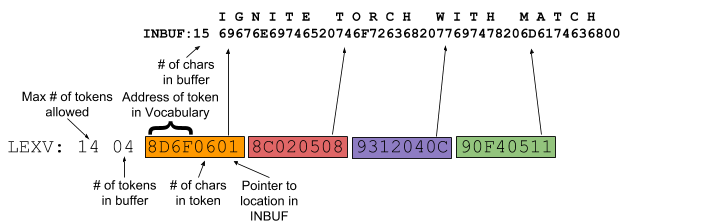
\includegraphics[width=1\textwidth]{figures/InbufAndLEXV}

\caption{INBUF and LEXV}

\end{figure}


\subsection{PARSER Variables and Grammatical Structure Definitions}

In \textquotedblleft The Parser\textquoteright s Role\textquotedblright{}
section of \textquotedblleft Learning ZIL\textquotedblright , PARSER
takes the input and tries to identify the action number for PRSA and
the object numbers for PRSO (parser direct object) and PRSI (parser
indirect object). This is not quite correct. It will set PRSA with
the action referred by the verb in the input. However, PARSER does
not set PRSO or PRSI. The only exception is if the PRSA is GO. Then
the PRSO is set to the exit direction. The routine actually fills
two tables (P-PRSO and P-PRSI) with all the direct and indirect objects
requested in the command.

The basic grammar structure for a command is:
\begin{lstlisting}[basicstyle={\ttfamily}]
verb + prep + noun clause + prep + noun clause + end-of-command +
verb + prep + noun clause + prep + noun clause + end-of-command ...
\end{lstlisting}
Only the verb is required. All other parts are optional. A noun clause
is a noun or set of nouns connected by conjunctions (AND or commas).
These nouns can be modified by adjectives, quantifiers (ALL, A, or
ONE), or other special tokens excluding prepositions (OF, BUT, or
EXCEPT). The entire noun clause is referred as a direct or indirect
object clause. Prepositions are not included in the noun clause.

\medskip{}
For example:
\begin{lstlisting}[basicstyle={\ttfamily}]
DROP THE YELLOW BALL AND CROWBAR
INSERT A DOLLAR INTO THE RED SLOT 
TAKE ALL EXCEPT THE CANDLES
\end{lstlisting}

\texttt{THE YELLOW BALL AND CROWBAR}, \texttt{A DOLLAR, THE RED SLOT},
and \texttt{ALL EXCEPT THE CANDLES} are the noun clauses.

Individual commands can be connected together with end-of-command
tokens (THEN, AND,\texttt{ ,} or periods) that indicate where a command
stops. So:
\begin{lstlisting}[basicstyle={\ttfamily}]
DROP THE YELLOW BALL AND TAKE THE CROWBAR
DROP THE YELLOW BALL. TAKE THE CROWBAR
\end{lstlisting}
are equivalent to
\begin{lstlisting}[basicstyle={\ttfamily}]
DROP THE YELLOW BALL THEN TAKE THE CROWBAR
\end{lstlisting}
Commas can separate multiple objects in a single noun clause or indicate
the start of a new command. So:
\begin{lstlisting}[basicstyle={\ttfamily}]
DROP THE BALL, A RAKE AND SHOVEL
DROP THE BALL, TAKE THE SHOVEL
\end{lstlisting}
are processed differently based upon word type after the comma. More
in the details below.

\subsection{PARSER Table (ITBL)}

The main goal of PARSER is to extract the action (PRSA) and valid
objects in the direct and indirect object clauses from the given command.
To assist other routines in extracting this information, PARSER will
store specific information related to the verb, prepositions, and
location of noun clauses in a 10 word table, ITBL:\medskip{}

\begin{tabular}{|l|l|}
\hline 
Word 0 & Verb Number (VERB)\tabularnewline
\hline 
Word 1 & Verb Table Address (VERBN)\tabularnewline
\hline 
Word 2 & Prep Number (PREP1)\tabularnewline
\hline 
Word 3 & Addr of Prep (PREP1N)\tabularnewline
\hline 
Word 4 & Prep Number (PREP2)\tabularnewline
\hline 
Word 5 & Addr of Prep (PREP2N)\tabularnewline
\hline 
Word 6 & Start Addr of Direct Clause (NC1)\tabularnewline
\hline 
Word 7 & End Addr of Direct Clause (NC1L)\tabularnewline
\hline 
Word 8 & Start Addr of Indirect Clause (NC2)\tabularnewline
\hline 
Word 9 & End Addr of Indirect Clause (NC2L)\tabularnewline
\hline 
\end{tabular}

\medskip{}
The verb number is a unique value for similar meaning verbs in the
vocabulary. It is not the same as the action number. A verb will have
the same verb number no matter the context of its use but it could
have a different action number. For example, LOOK has the verb number
\$E9 in all syntaxes, but the action number for LOOK FOR is \$2D,
LOOK IN is \$3F, and LOOK is \$D0 corresponding to different types
of actions. The verb table contains the same information about the
verb as in the token buffer: verb\textquoteright s address (in Vocabulary),
length, and location in the input buffer (INBUF). The start and end
addresses of a clause refer to locations in the token buffer (LEXV).
Of note, this end address actually points to the token AFTER the last
included token in the particular clause.

\begin{figure}[H]

\includegraphics[width=1\textwidth]{figures/ParserTableLEXV}

\caption{Parser Table}

\end{figure}


\subsection{Checking Word Types with WT?}
\begin{description}
\item [{Arguments}] (Address, word type to match, word type to return)
\item [{Return}] ID value or FALSE if no match
\end{description}
WT? is one of the most important routines in Infocom games and sees
if the Vocabulary entry at the given address has the given word type.
This is the primary word type as described in Section 2.6. If the
primary word type does not match the given word type, WT? returns
with FALSE. If there is a match, the result returned depends on the
third argument. If no third argument is given, the routine will return
TRUE. If the third argument matches the secondary word type (as described
in Section 2.6), then the secondary ID is returned. Otherwise, the
primary ID is returned regardless if it is a valid word type for the
primary ID.\medskip{}

\begin{tabular}{|>{\centering}p{0.1\columnwidth}|>{\centering}p{0.1\columnwidth}|>{\centering}p{0.1\columnwidth}|>{\centering}p{0.1\columnwidth}|>{\centering}p{0.1\columnwidth}|>{\centering}p{0.1\columnwidth}|>{\centering}p{0.1\columnwidth}|>{\centering}p{0.1\columnwidth}|}
\hline 
\multicolumn{6}{|c|}{Primary word type} & \multicolumn{2}{c|}{Secondary word type}\tabularnewline
\hline 
Bit 7 & Bit 6 & Bit 5 & Bit 4 & Bit 3 & Bit 2 & Bit 1 & Bit 0\tabularnewline
\hline 
\$80 & \$40 & \$20 & \$10 & \$08 & \$04 & \$02 = Adjective & \$00 = Noun\tabularnewline
\hline 
Noun & Verb & Adjective & Direction & Preposition & Special & \$03 = Direction & \$01 = Verb\tabularnewline
\hline 
\end{tabular}

\medskip{}
Using:
\begin{verbatim}
$4386:3A 6B C4 D9 62 B5 B4
\end{verbatim}
the first 4 bytes are the z-string for \textquotedblleft inflat\textquotedblright .
\$62 indicates it is an verb and adjective. So,

\medskip{}

\texttt{CALL WT?(\$4386, \$40 or \$20)} will return TRUE

\texttt{CALL WT?(\$4386, \$40 or \$20, \$02)} will return the secondary
ID of \$B5.

\texttt{CALL WT?(\$4386, \$40 or \$20, \$00 or \$01 or \$03)} will
return the primary ID of \$B4.

\texttt{CALL WT?(\$4386, \$10)} will return FALSE as there is no match.

\medskip{}

Infocom games interestingly do not put the special ID values for directions,
verbs, or adjectives as the primary ID value when those tokens only
have one word type. For example, the Vocabulary entry for \textquotedblleft search\textquotedblright{}
is:
\begin{verbatim}
$4967:61 46 DD 0D 41 E0 00
\end{verbatim}
with the word type as 41 (primary type is verb, secondary type is
verb). The primary ID value is \$00 though. To get the verb number
(\$E0), you have to access the secondary ID by using \$03 as the third
argument:
\begin{verbatim}
CALL WT?($4967, $40, $01)
\end{verbatim}
Since a third argument is needed anyways to get an ID value, the designers
to just put it as the secondary ID value.

Almost everyone game uses the same WT? routine. So games did not even
use a separate routine but just hard coded the check when needed.
\textbf{LGOP} did add an additional word type check for nouns, \$80.
If it was found, the routine would quickly exit (no value is returned
for nouns) and bypass checking for secondary word types. \textbf{Sherlock}
uses the newer compressed Vocabulary entry format. Since secondary
word type checking happened mainly with prepositions, WT? only allowed
prepositions to be checked then when secondary word type arguments
are given. This is done by searching the Preposition table. If a match
is found the preposition value is calculated based upon the token\textquoteright s
position in the Preposition table. Internal Infocom notes mentions
a special WT? for \textbf{The Lurking Horror} where 3 ID values were
stored for each token, but no evidence of this can be found of this
routine in the 3 known game releases.

\subsection*{(Part 2) - Scanning Tokens}

\subsection{Start of PARSER: Where is the command? }

PARSER was able to understand single commands or multiple commands
separated by \textquotedblleft .\textquotedblright{} or THEN by parsing
them individually. It first decides if the next command should come
from the previously given input by seeing if P-CONT is set. This variable
contains the starting location of the next command\textquoteright s
first token from the previous input. This is set by seeing if more
tokens exist after a complete command is parsed. If P-CONT is clear,
PARSER then asks for new input from the user by printing \textquotedblleft >\textquotedblright{}
character and calling the READ opcode.

\subsection{Now, Traverse the Tokens\dots{}}

Because of the structure of accepted commands, PARSER can search for
a command in an efficient manner. It will walk through the tokens
and look for ones with specific parts of speech. If a noun clause
is found, PARSER will call another routine, CLAUSE, to find the start
and end tokens for the direct object clause. If no error is returned
by CLAUSE, PARSER will continue checking tokens and look for another
noun clause (indirect object clause) or end-of-command token. The
order for checking tokens is:
\begin{enumerate}
\item Invalid Token\\
All valid tokens have an address to their associated entry in the
vocabulary. Any invalid or unmatch tokens are given an address of
\$00. If this is found, an unknown-word error message will be printed
and FALSE returned.
\item End-of-Command Token\\
An end-of-command token (THEN or \textquotedblleft .\textquotedblright )
will stop the loop and jump to the post-looping processing. If there
are more tokens, PARSER will save the position of this next token
which PARSER will use for the next command.
\item Direction Token\\
This is the only verb with its own specific check in PARSER since
it is the most common command given. A direction token has an associated
direction value which is the property number for a room\textquoteright s
exits in that direction. There are 4 special scenarios where this
direction value is saved and the loop is stopped:\\
\\
1. This is a 1 token command, just the direction is given.\\
2. This is a 2 token command and the verb GO was already given (as
in \textquotedblleft GO EAST\textquotedblright ).\\
3. There are more tokens after the direction, and the next token is
a end-of-command token.\\
4. There are more tokens after the direction, and the next token is
a conjunction token (AND or \textquotedblleft ,\textquotedblright ).
If so, the conjunction token is changed to \textquotedblleft then\textquotedblright{}
to indicate a new command. So a series of direction commands separated
by commas or \textquotedblleft and\textquotedblright{} become separate
commands.\\
\\
PRSA is set to GO (if not already done). PRSO is later set to the
direction value. 
\item Verb Token\\
If a verb token is found, PARSER checks if a verb has already been
a found. A command cannot have two verbs. If no verb has already been
found, this verb\textquoteright s verb number and address to a verb
table that has the 4 byte token data are stored in words 0 and 1 of
ITBL. If a verb has already be found, PARSER will see if it the word
could also refer to a different valid part of speech.
\item Preposition, Quantity, Adjective, and Noun Tokens\\
Any of the above tokens indicates a noun clause is starting. The number
of noun clauses variable is incremented. A separate routine (CLAUSE)
will then find the end of the noun clause and store the start and
end addresses in ITBL. CLAUSE then returns the start address of any
remaining tokens PARSER should process. There are several exceptions
where CLAUSE is not execute:\\
\\
1. If the matched adjective or noun is followed by OF, PARSER will
ignore the adjective and noun and use the token after OF for the start
of the noun clause. This new token will be matched on a subsequent
loop.\\
2. If there are no more tokens or an end-of-command token is next
after the matched preposition and less than 2 noun clauses have been
found, the preposition address and value information will be save
into ITBL (Word 2 and 3).\\
3. If there are already 2 noun clauses, a \textquotedbl Too many
noun clauses??\textquotedbl{} error is given. PARSER will then return
with FALSE.
\item Special Token\\
Any remaining special tokens that do not affect the syntax or objects
requested will be ignored. This includes tokens like IS, YES, A, or
THE.
\item Improper/extra tokens - Syntax Error\\
All other situations are a syntax error. Therefore, PARSER will display
a can\textquoteright t-use-the-word error and return FALSE. examples?
\end{enumerate}
The first version of PARSER could understand multiple commands if
they were separated by THEN or \textquotedblleft .\textquotedblright .
Using AND or \textquotedblleft ,\textquotedblright{} between verbs
without objects like
\begin{verbatim}
JUMP AND LOOK
\end{verbatim}
were not understood. However, commands with objects separated by AND
or \textquotedblleft ,\textquotedblright{} like
\begin{verbatim}
OPEN MAILBOX AND GET LEAFLET
\end{verbatim}
are accepted as CLAUSE would realize the AND separates two commands.

\subsection*{(Part 3) - Updates (Actors, Adverbs, and Numbers) }

\subsection{Update: Speaking to Actors with Quotes}

The first modification to PARSER began with \textbf{Zork 2} and relates
to double quotes in commands. A double quote is treated like an end-of-command
token like THEN or period. It also toggles the QUOTE-FLAG which is
essentially a flag for finding an another double quote. The first
double quote seen sets that flag. A second will clear it.

In \textbf{Zork 2}, the use of a double quote comes into play in several
special situations.When the player says something out loud such as
SAY \textquotedblleft ABRACADABRA\textquotedblright , the game will
typically ignore these commands unless you are saying special words
for a spell or a riddle. The game will then pull out the word after
the first double quote and use it to trigger other routines.

PARSER will also handle speaking to the other actors using quotes.
Actors are characters in the game that can be asked questions or perform
actions. They are created using objects and have the PERSONBIT set.
Using interrupts, the game can have the actors move or perform other
actions on their own. To have an actor perform an action like:
\begin{verbatim}
TELL WIZARD "TURN OFF THE LAMP"
\end{verbatim}
PARSER first divides up the command into two separate commands with
the double quote as the terminating token for both commands. So the
previous command becomes:

\medskip{}
\texttt{TELL WIZARD''} and

\texttt{TURN OFF THE LAMP''}

\selectlanguage{american}%
\medskip{}

To have actors perform actions, PERFORM (discussed later) will call
the TELL/ASK routine first which ensure the direct object is a person
(PERSONBIT) and then set WINNER to the actor. PARSER will then process
the second command with the actor as the WINNER. The individual action
routines handle these special situation where actors perform the commands
by checking the value of WINNER. Later, PARSER will ensure that WINNER
is set back to the player on its next execution by detecting a clear
QUOTE-FLAG and WINNER not set to the player. 

\textbf{Deadline} expanded the methods for interacting with actors
by allowing commands in these formats:

\medskip{}

\texttt{TELL/ASK }\texttt{\textsl{actor}}\texttt{ TO }\texttt{\textsl{command}}

\texttt{\textsl{Actor}}\texttt{ THEN }\texttt{\textsl{command}}

\medskip{}

PARSER would change the TO or THEN tokens to a double quote token
which is then treated as an end-of-command token just like it was
back in \textbf{Zork 2}. The verb number in ITBL would automatically
be set to the verb number for TELL if the second format is used. \textbf{HGTG}
later added a check to ensure the token after TO was a verb which
indicated the start of another command.

The player in \textbf{Deadline} could also refer to actors with their
name followed by a comma:\medskip{}

\texttt{\textsl{Actor, command}}

\medskip{}

PARSER (through CLAUSE) considers as a end-of-command between two
commands. The comma is then changed to \textquotedblleft then\textquotedblright{}
and processed like in the other formats.

Deadline also allowed the PLAYER to ask the actors directly about
an object or ask them to give you an object using:

\medskip{}

\texttt{ASK }\texttt{\textsl{actor}}\texttt{ ABOUT }\texttt{\textsl{object}}

\texttt{ASK }\texttt{\textsl{actor}}\texttt{ FOR }\texttt{\textsl{object}}

\medskip{}

These are treated like any other command and depend on the object
attributes.

Finally, \textbf{Deadline} also introduced a new routine which checks
if the requested actor is in the current location and if the subsequent
command is appropriate (action is WHAT, FIND, TELL, or SHOW) before
allowing the commands to be processed. This check would be added to
subsequent games.

PERFORM will call the TELL/ASK routine which ensure the direct object
is a person (PERSONBIT) and then set WINNER to the actor. PARSER will
then process the second command with the actor as the WINNER.

\subsection{Update: Titles and Adverbs (briefly)}

The recognition of titles used to address actors like MRS. or MR.
and automatically skip them along with any following period was introduced
with \textbf{Deadline}. The game also recognized 5 specific adverbs
(CAREFULLY, QUIETLY, SLOWLY, QUICKLY, and BRIEFLY) and saved the adverb\textquoteright s
Vocabulary address in ADVERB. It would be used later by specific action
routines such as WATCH, GO, or READ. The adverbs were considered a
special token and not a specific part of speech. \textbf{Bureaucracy}
is the only game with adverbs, but they are not needed to complete
the game.

\vfill{}

\pagebreak{}

\subsection{Update: Numbers, a new object}

Deadline introduce numbers and time to Infocom games. Since these
values do not match with any token, they are given a \$0000 Vocabulary
address. NUMBER? will then change the \$0000 to the vocabulary address
for a \textquotedblleft intnum\textquotedblright{} or \textquotedblleft number\textquotedblright{}
token. A special global variable contains the numerical value. For
time values, the time in minutes is saved:
\begin{enumerate}
\item Loop through all the characters of an unknown token
\item If the character is a digit, then take the current sum, multiply it
by 10, and add this value of this digit.
\item If a \textquotedblleft :\textquotedblright{} is found, then the previous
digits are likely an hour value. Save this into a separate TIM variable
and reset the total sum. Continue looping through the remaining digits
which will be the minutes value.
\item Once all the digits are read (and there are no extra non-digit characters),
then the sum (value of the digits) is save into P-NUMBER and this
unknown token is given the Vocabulary address for \textquotedblleft intnum\textquotedblright .
\item If the sum is greater than 10000, then the routine will return FALSE.
\item If the number was an time value, then the sum is actually the minutes
value. The routine will take the hour value and multiply it by 60
and then add the sum. If the hour value is greater than 23, then the
routine will return FALSE. There is no restriction on the size of
the minutes value though. This new sum (time in minutes) is also saved
in P-NUMBER.
\end{enumerate}
\begin{figure}[H]
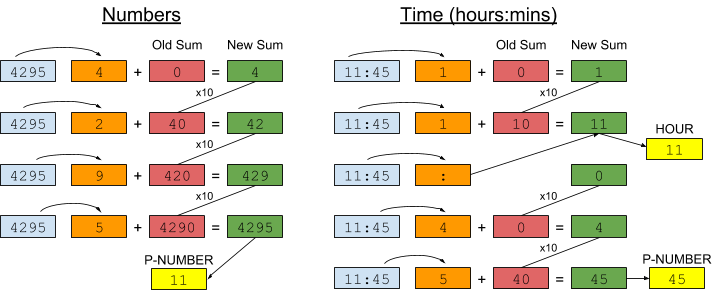
\includegraphics[width=1\textwidth]{figures/NumbersAndTime}

\caption{Numbers, Time}

\end{figure}

Routines can then search for the \textquotedblleft intnum\textquotedblright{}
token and use the value in the corresponding global variable. Because
of this design, only one number or time value could be used in each
command. Games using time values can impose certain restrictions on
the what hours are valid. For example, \textbf{Deadline} considers
any time between 1:00 and 7:59 to be PM. So 7:00 is converted to 19:00
(or 7pm) for the game. Hours from 0 to 23 are considered valid for
all games. Most games will convert the hour and minutes into all minutes.
Only \textbf{Sherlock} checks the value of the minutes. So a time
value of 14:80 could be valid in most games that use time as they
are converted to all minutes.

More number formats would be recognized in later games. They are listed
below:\medskip{}

\begin{tabular}{|>{\raggedright}p{0.25\textwidth}|>{\raggedright}p{0.25\textwidth}|>{\raggedright}p{0.4\textwidth}|}
\hline 
Added Format & Game Introduced & Notes\tabularnewline
\hline 
\hline 
\$xxx & Cutthroats & No cents portion is allowed. The value is saved in a different global
variable than P-NUMBER. The \textquotedblleft intnum\textquotedblright{}
object has it\textquoteright s property 11 set to \textquotedblleft amount
of money\textquotedblright .\tabularnewline
\hline 
xxx-yyyy & Suspect & The phone number is stored as two separate numbers in separate global
variables\tabularnewline
\hline 
xxx,xxx & LGOP & Comma separated number is converted to a single 4-6 digit number\tabularnewline
\hline 
xx(B-E) \$xxx.yy \#xxxx & Bureaucracy & Number followed by letters B-E indicates seat row and letter (4 times
row \# + seat letter converted to 0-3 value) and money value (converted
to cents) are saved in their own special global values. The object
type returned is \textquotedblleft intnum\textquotedblright{} except
for a money value where \textquotedblleft money\textquotedblright{}
is used. If a \# starts a number, it is ignored.\tabularnewline
\hline 
HH:MM AM/PM & Sherlock & The hour is converted to the corresponding 24 hour value. The entire
time is saved in the game\textquoteright s special time table format\tabularnewline
\hline 
\end{tabular}

\section{PARSER: New Commands and Routines}

\subsection{Introduction}

Ever since the first version of \textbf{Zork 1}, there has been an
AGAIN command. However, it basically used the previously saved PRSA,
PRSO, and PRSI in a PERFORM call. The use of EZIP allowed new routines
to be created to handle the various new buffers and provide new commands.
Starting with \textbf{AMFV}, a new method to manage the input and
token buffers allowed for a more sophisticated AGAIN command. The
game also introduced the OOPS command where unknown words in a command
could be corrected one by one. \textbf{Beyond Zork} added the UNDO
command which allows the user to \textquotedblleft go back\textquotedblright{}
one command.

Also two new buffers were created, AGAIN-LEXV and OOPS-INBUF, for
three new routines. In essence, they could be also considered previous
LEXV and previous INBUF, respectively.

\subsection{STUFF}
\begin{description}
\item [{Arguments:}] source buffer, destination buffer, length
\item [{Returns:}] TRUE
\end{description}
STUFF copies a set length of tokens from the source buffer to the
destination buffer. If no length is given, the maximum length (29
tokens) is used. First, the two bytes (maximum and actual number of
tokens) at the start of the token buffer are copied. Then all the
token buffer data is copied up to the amount requested. The routine
always returns TRUE. \textbf{Beyond Zork} was able to replace this
routine with a new opcode (COPY\_TABLE). \textbf{Sherlock} still used
STUFF.

\subsection{INBUF-STUFF}
\begin{description}
\item [{Arguments:}] source buffer, destination buffer
\item [{Returns:}] TRUE
\end{description}
INBUF-STUFF just copies the entire contents one character at at time
of the source input buffer to the destination input buffer. With XZIP,
\textbf{Beyond Zork} and \textbf{Sherlock} used a new instruction
(COPY\_TABLE) to handle this routines.

\subsection{New AGAIN command}

In Infocom games since \textbf{AMFV}, the AGAIN command is more formally
processed and checked specifically by PARSER. If it is given, several
checks are done before the old command is copied back and processed:
\begin{itemize}
\item Check that last command was not orphaned
\item Check that last command was valid
\item Check that the actor in last command is still present. This is to
ensure that any non-player actor is present if an actor direct command
is used again.
\item Check the subsequent token (if it exists) is not a end-of-command
token (THEN, AND. period, or comma). Then print the error message.
\end{itemize}
If all the above checks pass, PARSER copies the old input buffer from
OOPS-INBUF into INBUF. It does the same for the AGAIN-LEXV to LEXV.

If commands exist after an AGAIN command, the entire token and input
buffers are temporarily saved into reserve buffers, RESERVE-LEXV and
RESERVE-INBUF, respectively, because they would\textquoteright ve
been overwritten while performing the AGAIN command. The start of
the next command is also saved in RESERVE-PTR. The previous WINNER,
P-MERGED flag, and DIR (just in case) are restored from global variables.
The previous token and input buffers, AGAIN-LEXV and OOPS-INBUF, are
again copied back into LEXV and INBUF, respectively. Finally, OTBL
is copied back into ITBL. PARSER then continues to process the newly
restored command as normal. On the next iteration of PARSER, it will
detect that RESERVE-PTR is set and copy the remain command info from
RESERVE-LEXV and RESERVE-INBUF data back into LEXV and INBUF, respectively.
The next command starts in the restored data at the location indicated
by RESERVE-PTR.

\subsection{OOPS!}

The OOPS command was an important innovation in the era before copy
and paste were invented. Previously any commands with errors would
have to be completely re-typed with the correction. This was especially
painful for long or multiple commands. The user could correct any
errors with
\begin{verbatim}
OOPS <replacement token>
\end{verbatim}
If an unknown token is found, various values are calculated and stored
in OOPS-TABLE:\medskip{}

\begin{tabular}{|>{\raggedright}p{0.2\textwidth}|>{\raggedright}p{0.2\textwidth}|>{\raggedright}p{0.2\textwidth}|>{\raggedright}p{0.2\textwidth}|}
\hline 
Word 0 & Word 1 & Word 2 & Word 3\tabularnewline
\hline 
\hline 
Offset to unknown token in AGAIN-LEXV & Offset to start of command with unknown token in AGAIN-LEXV & Length of all token data in command with the unknown token & Offset to byte after the end of OOPS-INBUF\tabularnewline
\hline 
\end{tabular}

\medskip{}
PARSER will grab the Vocabulary address of the replacement token (after
OOPS) and replace it with the empty address in the unknown token\textquoteright s
entry in AGAIN-LEXV. Only the first token after OOPS is checked. An
error message is display if more tokens are given. INBUF-ADD is called
to appended the replacement token to the end of the OOPS-INBUF. That
routine will also store the replacement token\textquoteright s length
and updated pointer in OOPS-INBUF in the unknown token\textquoteright s
entry in AGAIN-LEXV. Finally the modified OOPS-INBUF and AGAIN-LEXV
are copied back into the INBUF and LEXV, respectively. PARSER then
resumes parsing the command as it normally does. If there is another
unknown word error in this just correct command, another OOPS can
be used to correct the next error. This can go on until all the errors
are fixed.

This feature has been present in all version 3 games since \textbf{Sorcerer}-R18,
and all version 4 and 5 games since its introduction.

\subsection{INBUF-ADD}
\begin{description}
\item [{Arguments:}] length of replacement token, ptr of replacement token
in INBUF, offset of unknown token in OOPS-INBUF
\item [{Returns:}] TRUE
\end{description}
INBUF-ADD is slightly more sophisticated. The characters for the referred
token in the first two arguments in appended to the end of OOPS-INBUF.
The pointer to the end of OOPS-INBUF is retrieved from the OOPS-TABLE
(or calculated using the data from the last token if it is not in
the OOPS-TABLE). The length of this replacement token and pointer
to it in OOPS-INBUF are copied back into the unknown token\textquoteright s
entry in AGAIN-LEXV.

\begin{figure}[H]
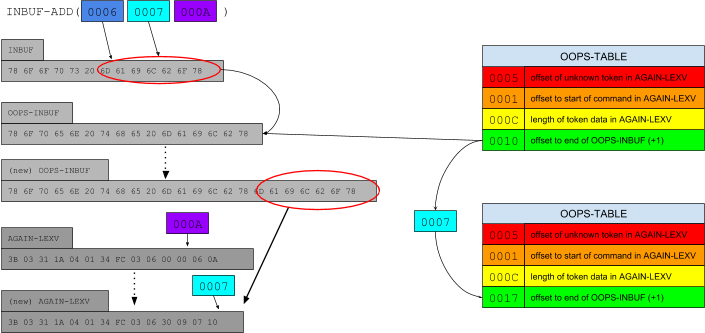
\includegraphics[width=1\textwidth]{figures/InbufAdd}

\caption{INBUF-ADD and OOPS-TABLE}
\end{figure}


\subsection{UNDO}

Finally an UNDO command was introduced with \textbf{Beyond Zork} which
would restore the game state before the last command was executed.
While this capability was available since version 1 of Z-machines,
it was never implemented because of the need for more internal memory
(a limited quantity back then) or having to constantly save the data
onto an external memory storage device, likely a disk drive, which
would slow the execution of the game down. But the requirements of
XZIP called for ZIP emulators with higher memory capacities, the necessary
game state data could be saved into a different part of the internal
memory. Only \textbf{Beyond Zork} and \textbf{Sherlock} had this function.

The saving of the current game state was done in the PARSER routine
after the check for a GO command. The save\_undo operation is used
to copy the contents of dynamic memory (everything before the Syntax
data) which is essentially the header information, all OBJECT data,
global variables, tables, and buffers. Also the call stack is saved.
If the player uses the UNDO command, it would call a separate routine
that would attempt to restore the saved gate state data and continue
with the execution of the command after the save\_undo operation in
PARSER. If an error occurs, the appropriate error message is displayed.

\subsection{Update: Other Minor Changes in PARSER}

EZIP and XZIP games only added slight modifications to PARSER. Most
of these revolved around setting or clearing certain global variables
such as XNAM. Others would search for unimportant tokens such as \textquotedblleft please\textquotedblright{}
and skip over them.

\subsection{Update: ReplaceToken routine}

With the advent of the AGAIN command in AMFV and its use of the AGAIN-LEXV
buffer, the replacing of tokens in PARSER and CLAUSE required changes
in both those buffers. So a new routine was created, ReplaceToken.
But it also including a way to copy the length and pointer information
for the token before the replaced one into the location of the replaced
one. The dictionary address for the replaced token will then be modified
as normal.

\section{CLAUSE: Find the Noun Clause Boundaries}
\begin{description}
\item [{Arguments:}] Start address of clause, Preposition number of clause,
Vocabulary address of current token
\item [{Return:}] Address to start of clause, -1 if no tokens are left
to process, or FALSE if error in clause syntax
\end{description}

\subsection{Introduction}

CLAUSE will find the end address of a noun clause and saves the start
and end addresses for this clause along with the preposition information
in ITBL. P-NCN (noun clause number) indicates if the direct (1) or
indirect (2) object clause is being processed. Specific locations
in ITBL for the extracted information to be stored are calculated
depending on P-NCN.\medskip{}

\begin{tabular}{|>{\raggedright}p{0.4\textwidth}|>{\centering}p{0.25\textwidth}|>{\centering}p{0.25\textwidth}|}
\hline 
 & Direct Object (Noun 1) Clause & Indirect Object (Noun 2) Clause\tabularnewline
\hline 
\hline 
Preposition Number & Word 2 & Word 4\tabularnewline
\hline 
Vocabulary Address of Preposition & Word 3 & Word 5\tabularnewline
\hline 
Address of First Token (Start) & Word 6 & Word 8\tabularnewline
\hline 
Address after Last Token (End) & Word 7 & Word 9\tabularnewline
\hline 
\end{tabular}

\pagebreak{}

\subsection{How it screens...}

CLAUSE loops through tokens in LEXV as long as the given tokens are
part of a valid syntax for a noun clause. Briefly, the routine will
\begin{itemize}
\item Save any preposition information (number and address) if it exists
into the proper locations in ITBL.
\begin{itemize}
\item The preposition information is usually passed as an argument. CLAUSE
will then find the Vocabulary address of the preposition.
\item If no preposition is given or exists, \$00 is saved as the preposition
number and address
\end{itemize}
\item Save the start address of the noun clause into the proper location
in ITBL.
\item Attempt to get the next token to process as well.
\item Loop through the tokens in LEXV as long as the given tokens are part
of a valid syntax for a noun clause (see rules below)
\end{itemize}
Once the routine stopped checking for tokens, it can return three
possible results: FALSE if there was a syntax error, -1 if no more
tokens left to process, or offset to the last token in the newly found
clause. The address after the end of the newly found clause will be
saved in the proper location in ITBL for the end address of the clause.\smallskip{}

\begin{tabular}{|>{\raggedright}p{0.3\textwidth}|>{\raggedright}p{0.3\textwidth}|>{\raggedright}p{0.3\textwidth}|}
\hline 
Type & Example & Action\tabularnewline
\hline 
\hline 
Unmatched &  & Display error \& return\tabularnewline
\hline 
Conjunction (\textquotedblleft and\textquotedblright{} or \textquotedblleft ,\textquotedblright ) & Eat apple \textbf{and} orange & Set ANDFLAG \& continue\tabularnewline
\hline 
Quantity (\textquotedblleft all\textquotedblright{} or \textquotedblleft one\textquotedblright ) & \textbf{Take all} bananas & Continue\tabularnewline
\hline 
Quantity (\textquotedblleft all\textquotedblright{} or \textquotedblleft one\textquotedblright )
+ \textquotedblleft of\textquotedblright{} & \textbf{Burn one of} the letters & Skip \textquotedblleft of\textquotedblright{} token \& continue\tabularnewline
\hline 
End-of-command \textquotedblleft then\textquotedblright{} or \textquotedblleft .\textquotedblright{} & Throw hammer \textbf{then} go west & Save end address of current noun clause and return\tabularnewline
\hline 
\hline 
Preposition (not the first token in the clause) & Put letter \textbf{inside} mailbox & Save end address of current noun clause and return\tabularnewline
\hline 
\hline 
Noun (also an Adjective) + Noun & Drop \textbf{gold coin} & Continue\tabularnewline
\hline 
Noun and ANDFLAG set & Eat apple and \textbf{orange} and grape & Clear ANDFLAG \& continue\tabularnewline
\hline 
Noun and ANDFLAG clear and next token is an exception (\textquotedblleft but\textquotedblright{}
or \textquotedblleft exception\textquotedblright ) or conjunction
token & Eat \textbf{apple} and orange \\
Eat all \textbf{fruit} except banana & Continue\tabularnewline
\hline 
Noun & Turn \textbf{statue} & Save end address of current noun clause \& return\tabularnewline
\hline 
\hline 
Adjective & Read \textbf{brown} book & Continue\tabularnewline
\hline 
\hline 
Special (not Conjunction, Quantity, or End-of-command) & Push \textbf{the} button & Continue\tabularnewline
\hline 
\hline 
All others (verbs or direction) and ANDFLAG set & Ignite red match and \textbf{go} east & Change conjunction token to \textquotedblleft then\textquotedblright{}
and go back 2 tokens to process again{*}\tabularnewline
\hline 
All others (verbs or direction) and ANDFLAG clear & Cut rope \textbf{go} north & Display \textquotedblleft Can\textquoteright t Use\textquotedblright{}
error \& return\tabularnewline
\hline 
\end{tabular}

\pagebreak{}
\begin{flushleft}
{*}For example:
\begin{lstlisting}[basicstyle={\ttfamily},showstringspaces=false,tabsize=1]
get candle and eat apple
             ^
\end{lstlisting}
\par\end{flushleft}

\begin{flushleft}
is converted to:
\par\end{flushleft}

\begin{lstlisting}[basicstyle={\ttfamily},showstringspaces=false,tabsize=1]
get candle then eat apple
         ^
\end{lstlisting}

with CLAUSE going back to the conjunction token to reprocess the clause.
The routine will recognize \textquotedblleft then\textquotedblright{}
as an end-of-command token, marking the end of a clause.

\vfill{}


\subsection{Update: New Matches\dots{}}

Later Infocom games added more acceptable token combination for clauses
which caused CLAUSE to also grow. Outside of specialized tokens used
in specific games (such as spell names in Spellbreaker), the new and
improved CLAUSE mainly became more sophisticated on deciding what
part of speech a token was being based upon its context with other
tokens. The major additional rules created by Infocom are below:

\medskip{}

\begin{tabular}{|>{\raggedright}p{0.25\textwidth}|>{\raggedright}p{0.25\textwidth}|>{\raggedright}p{0.25\textwidth}|>{\raggedright}p{0.15\textwidth}|}
\hline 
Type & Example & Action & Game\tabularnewline
\hline 
\hline 
Articles (\textquotedbl the\textquotedbl ,\textquotedbl a\textquotedbl ,\textquotedbl an\textquotedbl ) & Eat \textbf{an} apple & Skip over token \& continue & Deadline\tabularnewline
\hline 
Unmatched and NUMBER? is true & Take 2 candles & Unmatched token changed to \textquotedblleft intnum\textquotedblright ,
global var set to value, \& continue & Deadline\tabularnewline
\hline 
\textquotedblleft of\textquotedblright{} and verb = \textquotedblleft accuse\textquotedblright{} & Accuse Bob \textbf{of} murder & Change \textquotedblleft of\textquotedblright{} to \textquotedblleft with\textquotedblright{}
\& continue & Deadline\tabularnewline
\hline 
\textquotedblleft .\textquotedblright{} and previous token is a title
(\textquotedblleft mrs\textquotedblright ,\textquotedblright mr\textquotedblright ,\textquotedblright ms\textquotedblright ,
\textquotedblleft dr\textquotedblright , \textquotedblleft st\textquotedblright ) & Ask Mr. Smith about paper & Continue & Deadline, LGOP\tabularnewline
\hline 
\hline 
Preposition (first token checked) & Throw \textbf{out} ball & Continue & Zork 1-R88\tabularnewline
\hline 
Preposition (prep value already given in argument) &  & Skip over token \& continue & LGOP\tabularnewline
\hline 
Preposition (can also be an adjective) and a prep has already been
give & Write on \textbf{back} side & Assume preposition is an adjective and continue & Bureaucracy\tabularnewline
\hline 
\hline 
Noun (can also be adjective) and next token is noun or adj or direction & Drop \textbf{gold} coin\\
Take \textbf{copper} hot rod & Assume noun is an adjective \& Continue & HGTG, Moonmist\tabularnewline
\hline 
\hline 
Adjective AND P-MERGED/ P-OFLAG set or verb given & \textbf{Green}\\
Get \textbf{Green} & Continue & Zork 1-R88\tabularnewline
\hline 
\hline 
Special (not Conjunction, Quantity, or End-of-command) AND P-MERGED/
P-OFLAG set or verb given & \textbf{A} red\\
Get \textbf{a} red & Continue & Zork 1-R88\tabularnewline
\hline 
\hline 
All others (verb, direction) and ANDFLAG set and verb given & Ignite red match and \textbf{go} east & Change conjunction token to \textquotedblleft then\textquotedblright{}
and go back 2 tokens \& continue & Seastalker\tabularnewline
\hline 
\hline 
Profanity, interrogatives & Eat banana \textbf{who} & Display error message \& stop & LGOP, Trinity\tabularnewline
\hline 
\end{tabular}

\section{ORPHAN-MERGE: Fix What Is Broken}
\begin{description}
\item [{Arguments:}] None
\item [{Return:}] TRUE if orphaned command is corrected, FALSE if unable
to correct the orphaned command
\end{description}

\subsection{Introduction}

Now that the major parts of the command have been identified (if they
exist) and stored in ITBL, PARSER will first see if the given command
corrects an orphaned command, a previous command that had ambiguous
or missing necessary information. Originally, only nouns could be
ambiguous. So the clarifying token had be an adjective. If an adjective
could refer to more than one object in a location, an error was given.

For example, the user enters:

\begin{lstlisting}[basicstyle={\ttfamily}]
IGNITE CANDLE
\end{lstlisting}

in an empty room. An orphaned command will be created as no indirect
object is given (the candle needs to be ignited with something). The
game will respond that it does not know what the user wants to ignite
the touch with. This could be correct by then typing:

\begin{lstlisting}[basicstyle={\ttfamily}]
TORCH
\end{lstlisting}
 or 

\begin{lstlisting}[basicstyle={\ttfamily}]
WITH THE TORCH
\end{lstlisting}

A new command IGNITE CANDLE WITH TORCH would be created and replace
the previous command TORCH (or WITH THE TORCH) and then processed
by PARSER.

In another example, a room contains a red card, red flower, and blue
flower. If the command was

\begin{lstlisting}[basicstyle={\ttfamily}]
GET FLOWER
\end{lstlisting}

it would be considered ambiguous as it could be the red or blue flower.
This could be corrected by typing:

\begin{lstlisting}[basicstyle={\ttfamily}]
RED
\end{lstlisting}

which would then lead to a newly created command:

\begin{lstlisting}[basicstyle={\ttfamily}]
GET RED FLOWER
\end{lstlisting}

If the command was

\begin{lstlisting}[basicstyle={\ttfamily}]
GET BLUE
\end{lstlisting}

GET-OBJECT which matches the token with an object would be able to
figure out you meant the blue flower as there is only one object with
the BLUE adjective. If the command was

\begin{lstlisting}[basicstyle={\ttfamily}]
GET RED
\end{lstlisting}

then GET-OBJECT would display a missing noun error as the game will
not create an orphaned command from an ambiguous adjective.

Starting with \textbf{HGTG}, ambiguous adjectives could be used to
create an orphaned command be later clarified with a noun. So the
previous example would prompt the game to ask you for clarification
on which RED object. These examples could be corrected by typing just
CARD or FLOWER. So a clarifying noun could also refer to more than
one object in the same room which would then trigger another orphan
command. The game would then use the new information to match a single
specific object and process the newly completed command.

\subsection{Fixing Orphans with ORPHAN-MERGE}

ORPHAN-MERGE is called by PARSER if the P-OFLAG has been set in 2
possible situations:
\begin{itemize}
\item SYNTAX-CHECK is in unable to match even one syntax entries for the
given verb because of a missing object clause
\item GET-OBJECT is matches more than one object for the given noun, adjective,
or GWIM bit
\end{itemize}
Regardless of the outcome of the routine call, P-OFLAG will be cleared.
So the user only has one chance to supply missing or clarifying tokens
to an orphaned command. The orphaned command data is stored in OTBL
(a mirror of ITBL) and OCLAUSE (a mirror of LEXV).

ORPHAN-MERGE first validates the given input through various checks.
Only the missing or clarifying token is required. If any extra information
is given (like prepositions or verbs) are given, then they must match
the ones in the orphaned command to be accepted. ORPHAN-MERGE checks
two aspects of the given input:
\begin{itemize}
\item Verb - To be a valid response to an orphan command, the new input
must have the same verb as the orphaned command or must have no verb.
If the verb is different, the new input is likely a new command, and
ORPHAN-MERGE will return with FALSE.
\item Number of noun clause - Only one noun clause is allowed to clarify
an ambiguous or supply a missing noun clause. If two are given in
the new input, then ORPHAN-MERGE will return with FALSE.
\end{itemize}
ORPHAN-MERGE then checks if the orphaned command has a missing clause
by looking for \$01 in the starting address of the noun clauses in
OTBL. If both object clauses have starting addresses equal to \$01,
then only the direct object clause is processed. PARSER will then
attempt to process this partially completed command and again discover
this partially incomplete command can satisfy a syntax entry. If this
new command is again unable to be matched with a syntax, it will be
orphaned with the indirect object clause missing, The user can then
input another clarifying command for the indirect object clause.

Once a missing object clause is found, ORPHAN-MERGE will see ensure
that the preposition in the given input (if entered) matches the one
in the orphaned command (stored in OTBL). Finally, the routine will
copy the start and end addresses of the clarifying noun clause (the
single adjective) from LEXV into the appropriate start and end address
in OTBL. If the missing object clause is the indirect one, the number
of noun clauses will also be set to 2. ORPHAN-MERGE will then skip
checking if the given input clarifies an ambiguous noun.

\subsection{Clearing up Ambiguity}

If no missing noun clause found in OTBL (start address with \$01),
the given input could clarify an ambiguous noun. ORPHAN-MERGE checks
if P-ACLAUSE was set (by GET-OBJECTS) to the element of the clause\textquoteright s
start address in OTBL with the ambiguous noun (\$06 for direct object
and \$08 for indirect object clause). ORPHAN-MERGE will then proceed:
\begin{itemize}
\item Check that there is only one noun clause in the given input. If there
are more, than clear P-ACLAUSE and return with a FALSE.
\item Loop through the tokens in the noun clause indicated by P-ACLAUSE
and check their word types.
\item If the token\textquoteright s word type is an adjective, then temporarily
save the vocabulary address of that token. If an adjective has already
been found, the new one will override the old one. So only the last
given adjective is used for clarification.
\item If the token\textquoteright s word type is a noun, then ORPHAN-MERGE
ensures that the token is the same as the ambiguous noun (P-NAM) or
is \textquotedblleft ONE\textquotedblright . In the above example,
\textquotedblleft BLUE ONE\textquotedblright{} or \textquotedblleft RED
FLOWER\textquotedblright{} are both valid for the ambiguous FLOWER.
It will then stop checking tokens and call ACLAUSE-WIN (to create
a new noun clause)
\item All other word types or mismatched nouns will cause ORPHAN-MERGE to
stop checking tokens and return FALSE.
\item If no nouns are given after checking all the tokens in the given noun
clause, ORPHAN-MERGE will also call ACLAUSE-WIN using the last found
adjective in the given noun clause.
\item If no adjective is given after checking all those tokens, ORPHAN-MERGE
will return false.
\end{itemize}
Once any missing noun clause is replaced or an ambiguous word is clarified,
ORPHAN-MERGE will copy the data from OTBL into ITBL for PARSER to
continue to processing as if the complete command had just been entered.
So an clarified orphaned command will use tokens located in LEXV and
OCLAUSE.

\subsection{ACLAUSE-WIN}
\begin{description}
\item [{Arguments:}] Vocabulary address for Adjective
\item [{Return:}] TRUE
\end{description}
ACLAUSE-WIN setups up parameters for CLAUSE-COPY using ACLAUSE (element
number of a clause\textquoteright s start address such as \$06), ACLAUSE
+ 1 (element number of clause\textquoteright s end address such as
\$07), and the clarifying adjective. By setting the parse table that
CLAUSE-COPY should use (CC-TBL) to OTBL, CLAUSE-COPY will copy the
tokens from OCLAUSE back to OCLAUSE and insert a clarifying adjective
before the ambiguous noun (P-NAM). The routine will also ensure the
P-NCN is set to the correct number of noun clauses. ACLAUSE is cleared
to indicate the ambiguous noun was clarified.

\subsection{Using CLAUSE-COPY}
\begin{description}
\item [{Arguments:}] Element number of start address of clause in ITBL,
Element number of end address of clause in ITBL, INSERT adjective
(optional)
\item [{Return:}] TRUE
\end{description}
CLAUSE-COPY copies tokens from LEXV to the end of OCLAUSE using the
addresses in one of the parse table (ITBL or OTBL) referred by a global
variable (official name is not known). CLAUSE-COPY is called with
two arguments, the element numbers that identify the start and end
addresses for the noun clause to copy. These element values are \$06
and \$07 for the direct object clause or \$08 and \$09 for the indirect
object clause. It will then append the requested tokens to the end
of OCLAUSE.
\begin{itemize}
\item Find the offset to the end of OCLAUSE using the value in element 0.
\item Calculate the new start address of the orphaned noun clause by finding
the end address of OCLAUSE as it is the start address for the newly
appended tokens.
\item Store this new start address in the appropriate element (start address
for DO or IO clause) in OTBL (\$06 or \$08).
\item CLAUSE-COPY will repeatedly call CLAUSE-ADD to copy the tokens located
in the requested noun clause to the end of OCLAUSE. These new tokens
have their byte pointer to the input buffer and length set to zero.
\item If a clarifying token (usually an adjective) is given while copying
these tokens, CLAUSE-COPY will check if the copied token matches the
current ambiguous token, P-ANAM (a vocabulary address for the ambiguous
noun). If a match is found, CLAUSE-ADD is called with the vocabulary
address of ths clarifying token and a new token with the clarifying
token is added to OCLAUSE. Then the P-ANAM is also added to OCLAUSE
with CLAUSE-ADD.
\item Once all the remaining tokens in the requested noun clause are appended
to OCLAUSE, CLAUSE-COPY will calculate the new end address of OCLAUSE
and save it into the proper element (end address of noun clause) in
OTBL.
\end{itemize}
Starting with \textbf{Zork 1}, there was a bug with this setup. Each
time an orphaned noun clause was created, it was appended to OCLAUSE.
Since the end of OCLAUSE was never reset back to \$00, it was possible
OCLAUSE would grow outside of its 100 byte size limit and spill over
into the memory locations of other variables. This was correct with
\textbf{Zork 3} by setting the size of OCLAUSE to zero in the OPRHAN
routine.

\subsection{CLAUSE-ADD}
\begin{description}
\item [{Arguments:}] Vocabulary address to token
\item [{Return:}] True
\end{description}
CLAUSE-ADD takes the given Vocabulary address and creates a new token
add the end of OCLAUSE. Originally, the destination token buffer defaulted
to OCLAUSE. In \textbf{Moonmist}, the P-CCTBL was used to stored the
address of the destination token buffer in element 2. More information
about P-CCTBL in Section 10.10. In \textbf{Bureaucracy} (and later
\textbf{Beyond Zork}), the address of the destination token buffer
was passed as the 2nd argument instead of using P-CCTBL.

\subsection{Update: New changes of ORPHAN-MERGE}

First changes to ORPHAN-MERGE were with \textbf{Zork 1-R88}. It mainly
corrected the bug when a first token in a claifying response which
can be a verb and an adjective is matched as a verb first. This is
especially an issue when only the first 6 characters are used. For
example, the command:

\begin{lstlisting}[basicstyle={\ttfamily}]
BOARD BOAT
\end{lstlisting}

in a location with a row boat and inflatable boat in created an orphaned
command because BOAT is ambiguous. If the user then enters:

\begin{lstlisting}[basicstyle={\ttfamily}]
INFLAT
\end{lstlisting}

the original ORPHAN-MERGE processes INFLAT as \textquotedblleft inflate\textquotedblright ,
the verb, and asks what object to inflate. However, then this new
version will understand that the user meant an \textquotedblleft inflatable\textquotedblright{}
BOAT and treat INFLAT as an adjective to clarify the ambiguous BOAT.
Also, ORPHAN-MERGE will understand that the input:

\begin{lstlisting}[basicstyle={\ttfamily}]
INFLAT BOAT
\end{lstlisting}

means INFLAT is the adjective \textquotedblleft inflatable\textquotedblright{}
because the next token, BOAT, is a noun. INFLAT will then clarify
the ambiguous noun. Obviously, any token that can be a verb and adjective
will be treated as a verb by PARSER if there no orphan command to
clarify. \textquotedblleft ALL\textquotedblright{} and \textquotedblleft ONE\textquotedblright{}
are also considered valid adjectives for the purpose of clarification.
Finally, a new global variable, P-MERGED, is set if an orphaned command
is clarified and is used mainly when printing object names in PRSO/PRSI-PRINT
to ensure the whole correct object name is printed and not the clarifying
token.

\textbf{Planetfall-R37} introduced a similar dual word type option
for tokens which can be verbs and nouns. Early in the routine, the
given verb was checked for this dual word type. If it could be a noun,
then ORPHAN-MERGE assumed it should be treated as a noun. The start
address of the subsequent noun clause was adjusted to include the
previously thought verb. For example:

\begin{lstlisting}[basicstyle={\ttfamily}]
IGNITE TORCH
\end{lstlisting}

which will result in a missing noun error (need an indirect object).
If the user then types:

\begin{lstlisting}[basicstyle={\ttfamily}]
FIRE
\end{lstlisting}

this token can be a verb or noun. but will be treated as a noun as
there is an orphaned command.

\textbf{HGTG} introduced the ability to clarify an ambiguous adjective.
In those situations, a clarifying noun is given. Previously, any noun
given in the clarifying clause is ignored (if it is the same one in
the orphaned command) or causes an error if its different. Now, ORPHAN-MERGE
will also look for a clarifying noun if the ambiguous word is an adjective.
NCLAUSE-WIN is called to complete the clarification. ONE and ALL are
valid adjectives or nouns and can clarify either ambiguous nouns or
adjectives. If either of these tokens follows another adjective, then
they should be considered a noun and call ACLAUSE-WIN immediately
with the given adjective as the clarifying token. Finally, there is
a new data structure, OVTBL, which holds the VTBL from original command
that was orphaned. Essentially, ORPHAN-MERGE copies back the information
from OVTBL into VTBL but sets OTBL\textquoteright s VTBL addr to VTBL
and not OVTBL. But the OTBL information will be copied back to ITBL.

Suspect reconfirmed the number of noun clauses in the fixed orphan
command by seeing if the OTBL\textquotedblright s IO\textquoteright s
start address is set. If also skipped out of ORPHAN-MERGE if it was
called while there are still unprocessed commands are given where
the next verb is \textquotedblleft tell\textquotedblright .

\textbf{AMFV} changed the checking of a given verb. If it is the same
as the orphaned command, then skip over checking it as a possible
an adj. If the given verb does not match, then ORPHAN-MERGE will check
to see if that token can also be an adj.

\textbf{Bureaucracy} did not include the NCLAUSE-WIN option but did
allow for the entire noun clause to be used to clarify the ambiguous
noun. This is done by setting the ADJ to \$01 which will cause CLAUSE-COPY
to insert the entire noun clause instead of just the adjective. It
also blocks certain adjectives for clarifications.

\textbf{The Lurking Horror} introduced the assumption that if a verb
is given without a noun clause, then the verb could be the clarifying
token. The start of the noun clause would then be adjusted to include
the verb token. Copying of OVTBL and OTBL is gone???

\textbf{Sherlock} did also check to see if a solo verb can be a noun.
If so, then the verb table is cleared and the start and end addresses
of the DO are set to include the verb token. Sherlock will adjusted
the end address of the DO clause to include the entire IO clause for
certain situations (<name> + TOMB or BOX + <adj/noun>).

\textbf{AMFV} changed the way that the clarifying input is used with
orphaned commands. The main new feature is clarifying an ambiguous
noun as well. ORPHAN-MERGE still begins with
\begin{itemize}
\item Check if the new input\textquoteright s verb (if given) matches the
one in the orphaned command or the given verb also can be an adjective.
If so, set the ADJ to \$01 for now.
\item Otherwise check if the given verb can also be a noun. If so and no
other nouns were given then set the start and end addresses of the
direct object clause to be those around the first token (address of
the first token and address of the second token). The verb \# and
addr to VTBl will be cleared.
\end{itemize}
After those possible scenarios are checked, the routine does the similar
checking as the first gen ORPHAN-MERGE. It first checks the scenarios
where a verb is given which could have different meanings.
\begin{itemize}
\item If the new verb is different than the old verb from OTBL, then return
false. The new input is probably a new command.
\item If the new verb can also be an adjective, then save it in ADJ just
in case.
\item If the new verb can also be a noun and no noun clauses are given,
then set the start and end addresses of the direct object clause to
point to the verb.
\end{itemize}
The routine then does a few more checks:
\begin{itemize}
\item Rechecks the verb in the new input (if it exists). If this new verb
is not the same as the one in the OTBL and it cannot also be an adjective,
then RFALSE (an error).
\item If there two noun clauses are given, then it is an error (can\textquoteright t
offer two answers to correct an orphaned command).
\end{itemize}
The first type of orphan correction is replacing a missing noun clause.
This is marked by \$01 as the start address of a noun clause. The
routine will check the direct object clause first and then the indirect
object clause if the direct object is not missing any information.
The routine cannot correct both clauses with a single command.
\begin{itemize}
\item Check that the preposition in the new input (if given) is the same
as the one in the orphaned noun clause. If it is not the same, then
return false.
\item If ADJ is set (which means the verb is can also be a clarifying adjective),
then set the start and end addresses of the missing noun clause in
OTBL to address of the first token in the token buffer. If the ADJ
is not set, then set the start and end addresses of the missing noun
clause in OTBL to the ones from the direct object clause in ITBL.
For a missing indirect object clause, the routine copies the start
and end addresses from the direct object clause in ITBL to the indirect
object clause in OTBL and sets the \# of noun clauses to 2.
\end{itemize}
If neither noun clause is missing, the routine will look for a clause
with an ambiguous token. In that situation, ACLAUSE has the field
\# for the clause with the ambiguous token whose vocabulary address
is in P-ANAM. The routine will make sure there is only 1 noun clause
to clarify the ambiguous token. If is no noun clauses given and any
verb in the new input cannot be an adjective as well, then it will
error. The routine will then walk through the tokens in the direct
object clause of the new input to find the appropriate clarifying
tokens for the orphaned command. Each token will be checked:
\begin{itemize}
\item A quantity token (ALL, EVERYT, ONE) - set current token as ADJ
\item An adjective type - set cur token as ADJ
\item ONE (after other tokens) - call ACLAUSE-WIN with ADJ and stop looping
\item A noun type - If it is the same as the ambiguous token, then call
ACLAUSE-WIN with ADJ. Otherwise, call NCLAUSE-WIN as the noun is a
clarifying token.
\end{itemize}
If END is blank (for some reason), then set \# of noun clause to 1,
set END to original BEG, and set BEG to 1 token block before END.
Once all the checking has been done, ORPHAN-MERGE will copy the info
from OVTBL back to VTBL and copy the OTBL info back to ITBL. P-MERGED
is then set to indicate the orphan command is probably fixed.

\subsection{Update: New ACLAUSE-WIN expands its options}

\textbf{Zork 1-R88} also began to use the OVTBL to hold the corresponding
verb info for the ambiguous noun. This would be used to later repopulate
VTBL and create a valid command with the clarified token and ambiguous
noun.

\textbf{HGTG} began to use the CC-TBL to hold parameters needed for
ACLAUSE-WIN. Theses were mainly the source and destination buffer.
This allowed other buffers besides OCLAUSE to be used. The dictionary
address of the clarifying adjective in INSRT was still the only passed
argument.

\textbf{AMFV} abandoned using CC-TBL because all of the needed values
could be passed as routine arguments.

\textbf{Bureaucracy} added an interesting twist if ACLAUSE-WIN was
called with a blank INSRT. In that situation, it is set to \$01 which
then causes CLAUSE-COPY to insert the entire direct object clause
of the recently entered clarifying command instead of a single token.
Lurking Horror got rid of this function.

\subsection{Update: NCLAUSE-WIN}
\begin{description}
\item [{Arguments:}] Nothing
\item [{Results:}] True
\end{description}
NCLAUSE-WIN is a new routine first used in HGTG that is used when
players were able to clarify an ambiguous adjective. It was not always
allowed after its introduction in HGTG. It always uses the direct
object clause from ITBL as the source (obviously as the clarifying
noun is the first any only object given in an input) and P-ACLAUSE
as the destination clause in OTBL. It also adjusts the number of noun
clauses if necessary. Since Trinity, newer version 4 games and all
version 5 games that did allow for ambiguous nouns used a version
that did not rely on CC-TBL to pass arguments to CLAUSE-COPY. This
could be done with the routine call arguments now.

This new version adds several more checks:

if there are no noun clauses and the given verb can be an noun, then
assume the verb is a noun actually and create a noun clause around
it. Also adjust the NCN to 1. It can then continue processing it.

It also looks for \textquotedblleft one\textquotedblright{} when checking
for nouns. Typically, \textquotedblleft one\textquotedblright{} is
usually an adjective. But if it follows after another adjective, then
it should be considered a noun and call ACLAUSE-WIN immediately.

\subsection{Update: New version of CLAUSE-COPY}

With \textbf{HGTG}, the destination addresses were added to P-CCTBL
in those situations where CLAUSE-COPY was need to copy tokens to something
other than OCLAUSE.\medskip{}

\begin{tabular}{|>{\raggedright}p{0.2\textwidth}|>{\raggedright}p{0.2\textwidth}|>{\raggedright}p{0.2\textwidth}|>{\raggedright}p{0.2\textwidth}|}
\hline 
Word 0 & Word 1 & Word 2 & Word 3\tabularnewline
\hline 
\hline 
Element \# for start address for source token buffer & Element \# for end address in source token buffer & Element \# for start address in destination token buffer & Element \# for end address in destination token buffer\tabularnewline
\hline 
\end{tabular}

\medskip{}
Also the tables with source and destination addresses were passed
to CLAUSE-COPY along with the clarifying adjective to insert. 

\textbf{LGOP} checked to see if the first token to add to the OCLAUSE
is the same as the clarifying token. If so, then don\textquoteright t
check to see if current token to copy is the ambiguous one. Just copy
it to OCLAUSE. \textbf{LGOP} also fixed the resetting of OCLAUSE ptrs
by moving all the recently added tokens to OCLAUSE to the front of
OCLAUSE.

\textbf{Moonmist} added more changes. First, it changed the parameters
in CCTBL to the address of the destination token buffer (such as OCLAUSE)
in word 2. No word 3 value is needed. Second, it also checked the
first token in the destination token buffer was the same as the clarifying
token when the ambiguous token is found while copying tokens. If so,
it would skip over adding this clarifying token but would add the
ambiguous token to the destination token. Finally, if the INSRT=\$01,
it would copy the entire direct object clause in the clarifying command
before the ambiguous token. This allows a phrase to be copied instead
of a signal token.

\textbf{Bureaucracy} did not have rely on CC-TBL for arguments as
it was written in ZIP 4 which allowed up to 7 arguments to be passed
to routines. CLAUSE-COPY past the address to the source and destination
input tables, elements for the start and end addresses for the tokens
to copy, source of the tokens, and the INSRT clarifying token if necessary
as arguments. It has a more sophisticated memory management system
though. If the end of the new clarified clause token buffer (OCLAUSE
for direct object and IClause for indirect object) is close to the
start of the clause that is going to be copied, the routine will not
the clarified clause token buffer but modify the source clause by
shifting over tokens to create space for the clarifying tokens to
be inserted. This is to prevent an overrun of the clause token buffer
into other buffers. Otherwise, it functioned very similar to the \textbf{Moonmist}.
It did skip over moving the recently added tokens in the destination
token buffer to the front of it if the source token buffer is the
same as the destination token buffer. This is because they will be
automatically inserted to the front of the destination token buffer.

\textbf{The Lurking Horror} allowed for a noun clause to be the clarifying
information, not just a token as in previous versions of CLAUSE-COPY.
Another argument, along with the original INSRT, to represent the
start and end addresses of the tokens to insert when the ambiguous
token is found.

\textbf{Beyond Zork} used the more simple version in \textbf{Moonmist}
but did not need CC-TBL like \textbf{Bureaucracy}.

\section{SYNTAX-CHECK: Find Correct Syntax Entry}
\begin{description}
\item [{Arguments:}] None
\item [{Return:}] TRUE if syntax matched, Syntax number if matched using
GWIM, or FALSE for all errors or orphaned commands
\end{description}

\subsection{Introduction}

Given the verb, any prepositions, and any direct and indirect clauses,
the game will need to see which valid syntax structure for the given
verb best matches. Different usages of the same verb can require different
prepositions and noun clauses (for example: TAKE LETTER, TAKE LETTER
FROM MAILBOX, TAKE LETTER TO BOB). These combinations are stored as
syntax entries. SYNTAX-CHECK will attempt to find the best match.
If no perfect match can be found, GWIM is called to try to replace
any needed missing objects. If that also fails to completely match
a syntax entry, an orphan command will be created with ORPHAN. 

\subsection{Hierarchy of Matching}

SYNTAX-CHECK will try to match the command\textquoteright s combination
of verb, prepositions, and object clauses with one of the verb\textquoteright s
syntax entries. If it cannot find a perfect match because of missing
information, it will return the best fitting entry based upon a specific
hierarchy.

First, SYNTAX-CHECK will check if a verb is given. If not, then show
an missing verb error and return FALSE. Up to 2 noun clauses are allowed
in a syntax entry. If SYNTAX-CHECK finds a complete match as it loops
through all the verb\textquoteright s syntax entries, it will return
that syntax entry\textquoteright s action number.

\subsection{GWIM (Get What I Mean)}
\begin{description}
\item [{Arguments:}] GWIMBIT number, LOC byte
\item [{Return:}] Object number if only 1 match, False if no or more than
1 object matched
\end{description}
If there is no complete match, SYNTAX-CHECK will call GWIM to try
to match any missing object clauses with a local object to create
a complete match, favoring a missing direct object clause over indirect
object. For example, the command IGNITE PAPER would typically cause
an error as the game does not know what object to use to ignite the
paper (the indirect object clause is missing). GWIM uses GET-OBJECT
to search for a local object that has a specific attribute flag (GWIMBIT)
set and returns that object. In that example, the GWIMBIT would be
the attribute to indicate an object is a source of fire. If a local
object was a TORCH and it was on fire, then GWIM would display the
clarification and return TORCH:

\begin{lstlisting}[basicstyle={\ttfamily}]
IGNITE PAPER
[with the torch]
\end{lstlisting}

GWIM first checks if the passed GWIMBIT is the RMUNGBIT (AKA KLUDGEBIT).
If so, the ROOMS object is returned. After setting the global SLOCBITS
and GWIMBIT variables and resetting the number of objects in the MERGE
table, GET-OBJECT will try to match any object in the current location
with a GWIMBIT set. If none or more than 1 object is found, then return
false. If only 1 object is matched, then return that object. Also,
GWIM will display a small amount of text in parentheses or brackets
to describe which object was matched. It may also have additional
text to clarify the matched objects (for example, if it is in your
hand).

\newpage{}

\subsection{ORPHAN: Creating an Orphaned Command}
\begin{description}
\item [{Arguments:}] Address of syntax entry with missing direct object,
Address of syntax entry with missing indirect object
\item [{Return:}] True
\end{description}
If a the command given or completed by using GWIM does not completely
match any valid syntax entries, SYNTAX-CHECK will call ORPHAN to setup
an orphaned command. It is also called by GET-OBJECT (described later)
if too many objects match the given adjective and noun in a clause.
ORPHAN will first copy the data from ITBL to OTBL. If an indirect
object clause is given (possibly has ambiguous words), the indirect
object tokens from LEXV are appended into OCLAUSE. Then, if a direct
object clause is given (possibly has ambiguous words), the direct
object tokens from LEXV are appended into OCLAUSE. So the indirect
object tokens are placed before the direct object tokens in OCLAUSE.
When called by SYNTAX-CHECK, it also copies the corresponding preposition
number (if any) for the missing noun clauses into the OTBL. ORPHAN
then stores \$01 as the start address of the missing or ambiguous
noun clauses in the OTBL to indicate that clause has a missing or
ambiguous word. Finally, SYNTAX-CHECK will then set the O-FLAG and
offer clarifying information for the player to help supply the missing
information.

\begin{figure}[H]
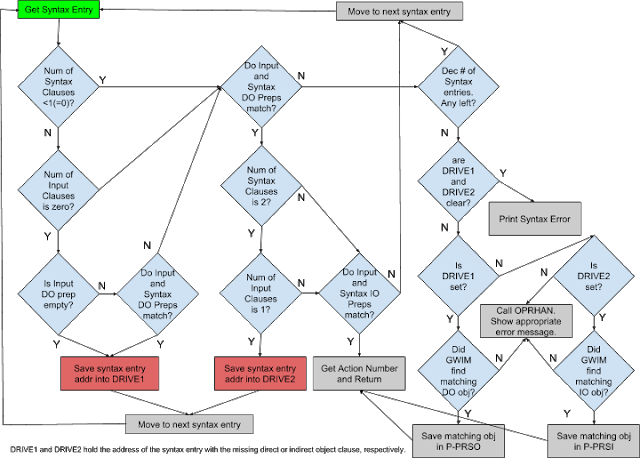
\includegraphics[width=1\textwidth]{figures/SyntaxCheck}

\caption{Syntax Check}
\end{figure}

\newpage Possible Outcomes:\medskip{}

\begin{tabular}{|>{\raggedright}p{0.2\textwidth}|>{\raggedright}p{0.2\textwidth}|>{\raggedright}p{0.2\textwidth}|>{\raggedright}p{0.2\textwidth}|}
\hline 
Syntax Entry Command & 0 object clauses & 1 object clause & 2 object clauses\tabularnewline
\hline 
\hline 
0 object clauses & All prepositions should be all blank. Return Action number & If DO preposition matches or command preposition is missing, then
DO Is missing. Save syntax entry address in DO missing var. & If DO preposition matches or command preposition is missing, then
DO is missing. Save syntax entry address in DO missing var.\tabularnewline
\hline 
1 object clause & All prepositions should be all blank. Return Action number & If DO preposition matches and indirect object preposition is blank,
then get Action number & If DO preposition matches, then IO is missing. Save syntax entry address
in IO missing var.\tabularnewline
\hline 
2 object clauses & All prepositions should be all blank. Return Action number & If DO preposition matches and indirect object preposition is blank,
then get Action number & If direct and indirect object prepositions match, then get Action
number\tabularnewline
\hline 
\end{tabular}

\subsection{Update: SYNTAX-CHECK}

No major changes were made in SYNTAX-CHECK except for a check on the
number of noun clauses in the input. If it was greater than the number
in the syntax entry, then it would bypass checking for orphaned clauses
as it isn\textquoteright t possible. Also, the error messaging was
more specific depending on what piece of information was missing such
as using \textquotedblleft WHO\textquotedblright{} or \textquotedblleft WHERE\textquotedblright{}
when appropriate and if the WINNER Is the PLAYER or a different actor.
Some games check for specific verbs that will not generate an orphaned
command.

\textbf{Mini-Zork} did use a new compact format for the syntax entries
that was also used in \textbf{Sherlock}. No other released Infocom
game used it. The size of the entry depended on the number of objects
in the entry. The number of objects is stored in the highest 2 bits
of byte 1. The preposition number for the direct object is reduced
by \$C0 and stored in the lower 6 bits of byte 1. The preposition
number for the indirect object is also reduced by \$C0 and stored
in the lower 6 bits of byte 5. However, the top 2 bits are not used
in byte 5. The syntax token byte is composed to flags that refer to
the LOC tokens referred earlier.

The structure of the syntax entries for no objects is:

\begin{tabular}{|>{\raggedright}p{0.2\textwidth}|>{\raggedright}p{0.1\textwidth}|}
\hline 
Byte 1 & Byte 2\tabularnewline
\hline 
\hline 
2 high bits = number of object clauses\\
6 low bits = Preposition number for direct object & Action number\tabularnewline
\hline 
\end{tabular}

\newpage The structure of the syntax entries with only direct objects
is:

\begin{tabular}{|>{\raggedright}p{0.2\textwidth}|>{\raggedright}p{0.1\textwidth}|>{\raggedright}p{0.1\textwidth}|>{\raggedright}p{0.1\textwidth}|}
\hline 
Byte 1 & Byte 2 & Byte 3 & Byte 4\tabularnewline
\hline 
\hline 
2 high bits = number of object clauses\\
6 low bits = Preposition number for direct object & Action number & GWIMBIT number for direct object & LOC byte for direct object\tabularnewline
\hline 
\end{tabular}

\medskip{}
The structure of the syntax entries with direct and indirect objects
is:

\begin{tabular}{|>{\raggedright}p{0.2\textwidth}|>{\raggedright}p{0.1\textwidth}|>{\raggedright}p{0.1\textwidth}|>{\raggedright}p{0.1\textwidth}|>{\raggedright}p{0.1\textwidth}|>{\raggedright}p{0.1\textwidth}|>{\raggedright}p{0.1\textwidth}|}
\hline 
Byte 1 & Byte 2 & Byte 3 & Byte 4 & Byte 5 & Byte 6 & Byte 7\tabularnewline
\hline 
\hline 
2 high bits = number of object clauses\\
6 low bits = Preposition number for direct object & Action number & GWIMBIT number for direct object & LOC byte for direct object & Prep number for indirect object & GWIMBIT number for indirect object & LOC byte for indirect object\tabularnewline
\hline 
\end{tabular}

\medskip{}
These variable sized entries help eliminate any wasted space in the
syntax entry blocks. SYNTAX-CHECK and SYNTAX-FOUND were adjusted to
use this different format.

\subsection{Update: New versions of GWIM}

Many games used modified GWIM routines that would add extra clarifying
text such as \textquotedblleft of\textquotedblright , \textquotedblleft at\textquotedblright{}
or \textquotedblleft in\textquotedblright{} when commenting to the
user about an object matched because of a command with a specific
preposition. \textbf{The Witness} would use a special string to refer
to an object matched by GWIM instead of the standard object name.
For example, GWIM will use \textquotedblleft Asian man\textquotedblright{}
preceded by \textquotedblleft the\textquotedblright{} instead of the
object\textquoteright s name, \textquotedblleft Mr. Phong\textquotedblright .
\textbf{Trinity} introduced an initial check of the GWIMBIT in the
IT-OBJECT if it is set to an object. The routine will return what
the object that is referenced by IT-OBJECT.

\subsection{Update: New versions of ORPHAN}

\textbf{HGTG} introduce a new method for handling orphaned commands
with the introduction of the game\textquoteright s new CLAUSE-COPY
(see above). For its ORPHAN routine, it made sure OCLAUSE was cleared
if P-MERGED is also clear and also copied over VTBL to OVTBL.

\textbf{Mini-Zork} has a modified ORPHAN because it uses a modified
syntax entry format. Instead of manually getting the preposition number
from the syntax entry, \textbf{Mini-Zork} calls a separate routine
that extracts is from the modified syntax entry format. Version 4
and 5 games could call CLAUSE-COPY with more arguments and needed
fewer global variables. So CC-TBL was not needed anymore. Version
5 games used the same routine as the Version 4 games but using the
COPY-TABLE command that replaced the manual copying loop in ORPHAN.

\textbf{Bureaucracy} uses the same routine as \textbf{AMFV} except
it copies the object clauses into separate token buffers, OCLAUSE
for the direct object tokens and IClause for the indirect object tokens.

\section{Getting Objects with SNARF-OBJECTS}
\begin{description}
\item [{Arguments:}] None
\item [{Return:}] TRUE if objects found, FALSE if no objects found
\end{description}

\subsection{Introduction}

After finding the best syntax entry and any local objects to represent
missing objects in the given command, SNARF-OBJECTS looks for the
objects mentioned in the direct and indirect object clauses by calling
two other routines on each clause:

SNARFEM to find all the objects mentioned in the noun clause

BUT-MERGE to remove all the exception objects not wanted by the user

The matched objects have their numbers stored into the appropriate
tables, P-PRSO and P-PRSI.

\subsection{Setting up Routines}

SNARF-OBJECT simply sets up the variables needed by SNARFEM: start
and end addresses of direct object clause and address of table to
store extracted objects, P-PRSO. After calling SNARFEM, BUT-MERGE
is called to remove any exception objects from BUTTABLE if any exists.
This is repeated using the indirect object clause and P-PRSI. If there
is only one object in P-PRSI and there are exception objects, SNARF-OBJECT
assumes the exception objects will apply to the P-PRSO and call BUT-MERGE
again on P-PRSO. For example, the command:

\begin{lstlisting}[basicstyle={\ttfamily}]
CUT ALL EXCEPT NEWSPAPER
\end{lstlisting}

is interpreted as multiple CUT commands on all the local objects except
the newspaper. Similarly, the command:

\begin{lstlisting}[basicstyle={\ttfamily}]
ATTACK ALL PIRATES WITH ALL GUNS EXCEPT RIFLE
\end{lstlisting}

has the RIFLE object removed from the indirect objects referenced
by ALL GUNS. However, the following command:

\begin{lstlisting}[basicstyle={\ttfamily}]
EAT ALL FRUITS WITH FORK EXCEPT APPLE
\end{lstlisting}

has the EXCEPT object applied to the direct objects this time as trying
to apply it to the indirect objects could actually eliminate the only
object in the indirect clause and generate an error.

\subsection{SNARFEM: Looking for Groups of Objects}
\begin{description}
\item [{Arguments:}] Start address to noun clause, End address to noun
clause, Address to object table
\item [{Return:}] True if objects extracted, False if no objects extracted
\end{description}
SNARFEM searches the noun clause for adjectives, nouns, and quantity
(like ALL or ONE) tokens that describe one object or a single group
of objects. Any found adjectives or nouns will have their values saved
in the global variables P-ADJ and P-NAM respectively. If multiple
adjectives or nouns are given, then only the most recent ones are
saved in those variables. Any other tokens like conjunctions, exceptions
(like BUT), or different quantity tokens indicate no more tokens to
describe an object and triggers GET-OBJECT to be called which matches
a local object with the given adjective and noun. Quantity tokens
change how many objects are matched by GET-OBJECT by changing GETFLAGS.
Exception tokens change where GET-OBJECT saves those matched objects.
Details are below:

\medskip{}

\begin{tabular}{|>{\raggedright}p{0.35\textwidth}|>{\raggedright}p{0.55\textwidth}|}
\hline 
Token & Action\tabularnewline
\hline 
\hline 
ALL & Set P-GETFLAGS to \$01 (ALL mode)\tabularnewline
\hline 
ALL + OF & Set P-GETFLAGS to \$01 (ALL mode) and skip over OF token\tabularnewline
\hline 
BUT or EXCEPT & If BUT table not being used, then call GET-OBJECT with TBL and switch
to BUT table for subsequent storage. Otherwise, call GET-OBJECT with
BUT.\tabularnewline
\hline 
A or ONE (no adjective set) & Set P-GETFLAGS to \$02 (ONE mode)\tabularnewline
\hline 
A + OF or ONE + OF (no adjective set) & Set P-GETFLAGS to \$02 (ONE mode) and skip over OF token\tabularnewline
\hline 
A or ONE (adjective already set) & Copy ONEOBJ into NAM. Call GET-OBJECT with the currently used table
(TBL or BUT).\tabularnewline
\hline 
AND or \textquotedblleft ,\textquotedblright{} & Call GET-OBJECT with the currently used table (TBL or BUT)\tabularnewline
\hline 
AND or \textquotedblleft ,\textquotedblright{} + AND or \textquotedblright ,\textquotedblright{} & Ignore first conjunction token and continue processing\tabularnewline
\hline 
Buzzwords & Skip over this token\tabularnewline
\hline 
OF (ALL, A, or ONE not given) & Set P-GETFLAGS to \$04 (INHIBIT mode). Ignore this object as it is
an error in syntax. Of note, PARSER already ignores any adjective
or noun with \textquotedblleft OF\textquotedblright{} at the start
of a clause.\tabularnewline
\hline 
Adjective & Set ADJ to adjective value and Dictionary address of adjective into
ADJN\tabularnewline
\hline 
Noun & Set Dictionary address of noun into NAM and ONEOBJ (just in case)\tabularnewline
\hline 
All other tokens & Skip over this token\tabularnewline
\hline 
No more tokens & Call GET-OBJECT with the currently used table (TBL or BUT)\tabularnewline
\hline 
\end{tabular}

\medskip{}
For example, ALL OF THE CANDLES is the treated the same as ALL CANDLES.
Also, A BLUE CARD AND A RED ONE is interpreted as A BLUE CARD AND
A RED CARD with ONE referring to the just given noun CARD. ONE OF
THE FLOWERS is seen as ONE FLOWERS.

If BUT or EXCEPT have not been given, any numbers for found objects
will be saved in table found in the third argument. Once BUT or EXCEPT
have been given, all found objects will be saved in BUT table.

\subsection{BUT-MERGE}
\begin{description}
\item [{Arguments:}] Address to object table
\item [{Return:}] P-MERGE (address to merged object table)
\end{description}
This routine copies the objects in the given table into the MERGE
table but skips over any objects in an exception (BUTS) table. It
uses ZMEMQ to see if the given object is in BUTS. While the routine
returns to address to the MERGE table. It will also put the address
of the given object table into MERGE.

\subsection{Getting Object Numbers for each Object with GET-OBJECT}
\begin{description}
\item [{Arguments:}] Address to Object table, Verbose flag
\item [{Return:}] TRUE if successful in getting appropriate number of object,
FALSE for any error
\end{description}
GET-OBJECT tries to find a local object that matches the given identifiers
(adjective, noun, and GWIMBIT) and stores that object number in the
given object table. It will limit the matched objects depending on
what GETFLAGS mode (default, ALL, ONE, or INHIBIT) is set by SNARFEM.
SLOCBITS is first set to \#FFFF (all flags set) to ensure the greatest
chance of matching an object to the identifiers. If a clause\textquoteright s
SLOCBITS is set to a non-zero value from the matching syntax and the
match mode is ALL, then that clause\textquoteright s SLOCBITS is used.

GET-OBJECT requires that a noun is at least given in the command.
If there is no noun, then the adjective will be used as a noun if
possible. For example, \textquotedblleft gold\textquotedblright{}
can be an adjective or a noun like in \textquotedblleft piece of gold\textquotedblright .
If the adjective cannot be a noun, the routine will display a missing
noun error and quit. Now, GET-OBJECT will look for objects in the
WINNER and current location (if lit) using DO-SL. Any found objects
are saved into the given object table. The processing of the objects
depends on the mode:
\begin{itemize}
\item ALL: Search using DO-SL and return true
\item INHIBIT: Return true
\item ONE: Search using DO-SL or GLOBAL-CHECK found:
\begin{itemize}
\item 0 objects (using DO-SL): Search again using GLOBAL-CHECK
\item 0 objects (using GLOBAL-CHECK): Give a CAN\textquoteright T SEE error
and return false.
\item 1 object: Return true.
\item >1 objects: Randomly pick one object and move it to the top of the
table. Set the number of objects to 1. Return true.
\end{itemize}
\item Default: Search using DO-SL or GLOBAL-CHECK found:
\begin{itemize}
\item 0 objects (using DO-SL): Search again using GLOBAL-CHECK
\item 0 objects (using GLOBAL-CHECK): Give a CAN\textquoteright T SEE error
and return false.
\item 1 object: Return true.
\item >1 objects: Restore SLOCBITS from matched syntax entry. Search again
with same method:
\begin{itemize}
\item 0 or >1 objects: Create an orphaned command by setting the ambiguous
variables (AADJ, ANAM, and OFLAG) and call OPRHAN (Initial search
had >1 but second search had 0 or >1 objects matched which is an ambiguous
situation.) Return false.
\item 1 object: Return true.
\end{itemize}
\end{itemize}
\end{itemize}
The identifiers, ADJ and NAM, are always cleared after GET-OBJECT
is called except if in INHIBIT mode. If a correct number of objects
is found, then the routine also restores the SLOCBITS to what is listed
in the matching syntax.

\subsection{Bug: Randomly Picking Objects}

When only one object is requested like in:

\begin{lstlisting}[basicstyle={\ttfamily}]
GET ONE CARD
\end{lstlisting}

in a room with multiple cards (blue card, red card, etc), GET-OBJECT
will randomly choosing one object. However, the routine places this
chose object in the first position of the object table. If there is
an object already in the first position, it will be overwritten. For
example:

\begin{lstlisting}[basicstyle={\ttfamily}]
GET FLASHLIGHT AND ONE CARD
\end{lstlisting}

SNARFEM will call GET-OBJECT on FLASHLIGHT and put that object number
in the first position of the object table. SNARFEM will then call
GET-OBJECT on ONE CARD. Since there are multiple cards in that room,
GET-OBJECT will randomly pick one and store it in place of FLASHLIGHT.

Another bug is that the randomly picked item could also picked outside
of the group of matching objects. For example:

\begin{lstlisting}[basicstyle={\ttfamily}]
GET FLASHLIGHT AND LETTER AND ONE CARD
\end{lstlisting}

in a room with three cards, GET-OBJECT will try to randomly pick one
of the three cards. If the random number is 1, GET-OBJECT will pick
the object in the first position which is FLASHLIGHT.

\subsection{Update: New versions of SNARF-OBJECTS}

\textbf{Zork 1-R88} added an P-AND flag to help with displaying lists
of objects properly and to have a hierarchy of adjectives when referring
to objects. Only the first adjective is used. All subsequent adjectives
are ignored before calling GET-OBJECT.

\textbf{Sorcerer-R18} processed the indirect clause first and then
the direct object clause. However processing the exception objects
is saved until the end with it trying to apply it to the direct object
clause first. If nothing happens then it will try to apply the exception
objects to the indirect objects. If there are no direct objects then
any exception clause will be applied to the indirect object. Most
of the games since the \textbf{Sorcerer-R18} had SNARFEM check if
P-GETFLAGS was in ALL mode before starting. If so, it would set GETFLAGS
back to ALL mode after completing its SNARFEM.

\textbf{LGOP} set a global variable, CurrentNounClause, which is used
by SNARFEM and SaveNAMAdj, when objects cannot be found. This allows
ambiguous nouns or adjectives for the direct and indirect clauses
to be stored separately. The game also added several more checks in
the routine. If an ALL, BOTH, or EVERYTHING token is found, the routine
will call MANY-CHECK to see if the syntax allows for multiple objects
to be processed. It also checks if the token is profane and provides
an error message. Finally, there is a check for certain adjectives.

\textbf{Bureaucracy} added a check on the number of indirect objects
if an exception was to be applied. If there is only 1 indirect object,
it would assume the exception objects would refer to the direct objects.
Trying to apply the exception objects on a single indirect object
could remove it.

\textbf{Sherlock} call SNARFEM and EXCEPTION on different clauses
depending on how many object clauses are in the syntax entry which
needs to be specially extracted with the compact format.???

\subsection{Update: New versions of SNARFEM}

\textbf{Sorcerer-R6} allowed special spell related word when referring
to objects. \textbf{Seastalker} similarly allowed numbers and also
had SNARFEM ignore any additional adjectives given when referring
to an object. Only the first adjective is used.

\textbf{HGTG} checks if the GETFLAGS was in ALL mode. If so, the GETFLAGS
is cleared (changed to default mode) and will restore the GETFLAGS
back to the ALL mode once SNARFEM is complete.

\textbf{LGOP} will check if a syntax entry will allow multiple objects
if \textquotedblleft all\textquotedblright{} or \textquotedblleft both\textquotedblright{}
is given with an object. It will be rechecked again toward the end
of the PARSER routine.

\textbf{Hollywood Hijinx} does allow for two adjectives to be given
for some objects and has a separate routine to check for valid combinations
when a second adjective is found.

Other games will have checks for profanity which is not allowed when
referring to objects.

\subsection{Update: New BUT-MERGE}

The only major change was with \textbf{AMFV} and other version 4 and
5 games was the use of SCAN\_TABLE operator instead of the ZMEMQ routine.
Though various parameters had to be calculated, the new operator could
quickly look for a found objects in the exception table.

\subsection{Update: New ways to GET-OBJECT}

Every game seems to have used their own special version of GET-OBJECT.
Those modifications included special checks for certain actions or
with certain objects and displaying special errors for certain situations.
However, improvements were made over successive games.

\textbf{Zork 1-R88} added a check if the WINNER is also the PLAYER
if there is an orphaned command. If so, then error that it can\textquoteright t
be orphaned.

\textbf{Zork 2-R23} added a new WHICH-PRINT routine which also lists
the possible objects for the user to choose from when the noun is
ambiguous. It also ensured that the PLAYER can also be checked for
objects if the WINNER needing objects is not the PLAYER.

\textbf{Zork 3} added an early check if the adjective could also be
a direction. If so, then it is saved in the DIR variable and ensures
the \textquotedblleft direction\textquotedblright{} object is the
only entry in the object table. More detailed error messages were
added for various situations.

\textbf{Suspended} had a unique GET-OBJECT as the player did not interact
directly with the environment. So the GET-OBJECT was more liberal
when searching for objects. It would ensure the SLOCBIT was \#FFFF
for all \textquotedblleft get\textquotedblright{} commands.

\textbf{The Witness} introduced the GENERIC property which contains
a routine address used to clarify a requested object. If multiple
objects match a given NAM instead of just one, the routine address
in the GENERIC property will be called. This routine will then try
to determine which specific object was requested based upon various
variable values and return that object number. There is no check to
see if the GENERIC property is set. If it is blank, it will just return
FALSE. GET-OBJECT will then default to providing an error message
and display the possible objects to choose from. Also, the NOT-HERE-OBJECT
was introduced. For any unmatching identifiers, the NOT-HERE-OBJECT
would be returned for counting purposes. The unmatched NAM and ADJ
are then saved into XNAM and XADJ.

\textbf{Planetfall} did all for searching the WINNER if in ALL mode
only if the WINNER was not the player.

\textbf{Sorcerer-R15} did limit the created of NOT-HERE-OBJECT and
XNAM/XADJ only if the room was lit or for specific actions.

\textbf{AMFV} introduced having a separate NAM and ADJ for direct
and indirect object clauses. They are stored in separate two word
tables with the first element in each is for the direct clause. It
was used by certain actions to check the current noun or adjective
in use. It use was later expanded in \textbf{LGOP}.

\textbf{LGOP} did save the identifiers for the direct and indirect
objects in different locations when an object is matched. It also
fixed the situation where the requested object is a vehicle that the
WINNER is inside of.

\textbf{Spellbreaker} also including the searching a vehicle for the
requested object if its open. In the few situations, that multiple
objects are matched, a separate routine is called to see if all the
objects have the same GENERIC routine. If so, the GENERIC routine
will be called to clarify which object was requested.

Some games will have extra checks for non-matched objects to see if
they are part of a special case. This is primarily for spell names.

\textbf{Bureaucracy} does add a creative error message if OCLAUSE
or IClause has more than 10 tokens in it.

\textbf{The Lurking Horror} saves the first 4 adjective identifiers
and their corresponding tokens for any object. If multiple adjectives
are given, it will see if the last one can also be a noun. If that
is the case, it will assign that token to NAM and decrease the number
of adjectives.

\section{Search for Objects using SEARCH-LIST}

\subsection{Introduction}

Another one of the interesting aspects of Infocom games is how it
searches and matches objects to those requested by the player. It
will use various methods to find these objects and collect them into
a table.

\subsection{SEARCH-LIST: Finding Objects in Room and on Winner}
\begin{description}
\item [{Arguments:}] Number to Object to search inside, Address to object
table, Search level (0-2)
\item [{Return:}] Number of objects found
\end{description}
When the user refers to objects in a command, PARSER needs to see
which objects are referred and accessible. The given noun, adjective,
and/or GWIMBIT will be used as identifiers for a particular object.
SEARCH-LIST will check the objects in a given location (a room or
person) and see if it matches these identifiers. There are 3 levels
of search which affects which objects are checked:
\begin{itemize}
\item Search-TOP/Type 0: ON-GROUND or HELD (reachable objects)
\begin{itemize}
\item Look at objects that are on \textquotedblleft top\textquotedblright{}
of all objects
\item Match against all non-container objects and objects on surfaces in
the location. Any containers (if they are open or transparent) and
surfaces on the surface are checked completely.
\end{itemize}
\item Search-ALL/Type 1 (all objects)
\begin{itemize}
\item Match against all objects in the location. Only containers that are
open or transparent will be searched.
\end{itemize}
\item Search-BOT/Type 2: IN-ROOM or CARRIED (contained objects)
\begin{itemize}
\item Look inside any containers (look at second-level or any non-top level)
\item Match against all objects on any surface and inside any open or transparent
container.
\end{itemize}
\end{itemize}
The matched objects are saved in the table addressed passed to SEARCH-LIST.

\newpage{}

\begin{figure}[H]
\begin{centering}
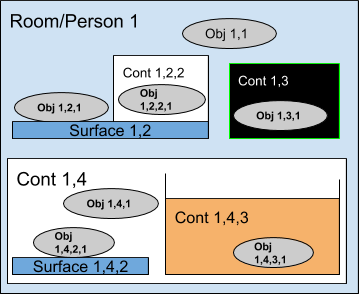
\includegraphics[width=0.5\textwidth]{figures/SearchObject}
\par\end{centering}
\caption{Search Object}

\end{figure}

For example, SEARCH-LIST is examining Room/Person 1. For each search
mode, the listed objects will be checked:

TOP: Obj 1,1, Surface 1,2 (Obj 1,2,1, Cont 1,2,2 (Obj 1,2,2,1))

BOT: Surface 1,2, Cont 1,4 (Obj 1,4,1, Surface 1,4,2 (Obj 1,4,2,1),
Cont 1,4,3 (Obj 1,4,3,1))

ALL: Obj 1,1, Surface 1,2 (Obj 1,2,1, Cont 1,2,2 (Obj 1,2,2,1)), Surface
1,2, Cont 1,4 (Obj 1,4,1, Surface 1,4,2 (Obj 1,4,2,1), Cont 1,4,3
(Obj 1,4,3,1))

Object Cont 1,3 is invisible.

All Infocom games appeared to be using the same SEARCH-LIST routine.

\subsection{DO-SL: Find Objects Based Upon Search Level}
\begin{description}
\item [{Arguments:}] Number of object to search, LOC value to SRC-TOP,
LOC value to SRC-BOT
\item [{Return:}] Number of objects found
\end{description}
DO-SL calls SEARCH-LIST with the appropriate search type depending
on the LOC flags given in the arguments and the LOC flags in the matched
syntax entry. If 1 is used for both DO-SL arguments then, SEARCH-LIST
will perform a SRC-ALL match. All matched objects will be saved in
P-TABLE.

GET-OBJECT calls DO-SL with the ON-GROUND and IN-ROOM flags to look
for any objects in the given location for use with the current syntax
entry. Similarly, GET-OBJECT also calls it with the HELD and CARRIED
flags to look for objects on the PLAYER. All other calls to DO-SL
seem to mainly use the double 1 parameter which will match anything.

All Infocom games appeared to be using the same DO-SL routine.

\subsection{GLOBAL-CHECK: Look for Objects Everywhere}
\begin{description}
\item [{Arguments:}] Address to object table
\item [{Return:}] True if GLOBALs checked, False if object matched from
local-globals or PSEUDO objects
\end{description}
Some objects in a game may be accessible from more than one locations
and valid objects to be used with certain actions. GLOBAL-CHECK is
the routine that tries to find these potentially valid objects. Infocom
had three different types of these special objects: GLOBALS, LOCAL-GLOBALS,
and PSEUDO objects.

GLOBALS can be accessed from any location in the game. If a game had
an AIR object, that would likely be accessible from any location.
Remember, these are not necessarily rooms. LOCAL-GLOBALS are accessible
from multiple locations but not all. The best example is a door which
would be accessible from the two rooms that are separated by it. PSEUDO
(or virtual) objects are the most confusing of the three objects as
they are not actual objects. They only have the SYNONYMS (nouns) and
ACTION properties. A given location can have PSEUDO objects that are
matched if certain nouns are used in that location. The routine then
jumps to a different routine for each noun that will figure out what
is the object the user was referencing. So a bed object in two different
rooms could be handled with a routine instead of creating multiple
objects.

GLOBAL-CHECK will first try to match any identifiers (noun/NAM, adj/ADJ,
or GWIMBIT) to any object in the GLOBAL property (AKA LOCAL-GLOBALS)
of the current location. The number to any matched objects will be
added to P-TABLE. The routine does not search inside the local-global
objects. Next, the PSEUDO property is checked which contains a list
of 2 word pairs. The first word is the Vocabulary address to the noun
that references the pseudo object while the second word is an ACTION
routine address. If the object matches, the Z-string of the matching
noun and ACTION addresses are saved into a pseudo object\textquoteright s
description and ROUTINE properties, respectively, which is then saved
to P-TABLE. GLOBAL-CHECK will continue to check the remaining objects
in PSEUDO and save any matches. If no objects have matched by this
point, the GLOBAL-OBJECTS are searched using DO-SL on GLOBAL-OBJECTS.
SLOC-BITS is temporarily set to \$FFFF which makes any match valid
and restored afterwards.

\subsection{THIS-IT?}
\begin{description}
\item [{Arguments:}] Object number
\item [{Return:}] True if object matches
\end{description}
Infocom games can use three different identifiers to see if an object
matches the one requested in a command: noun (P-NAM), adjective (P-ADJ),
and GWIMBIT. THIS-IT? will see if the given object matches any of
these identifiers. First, the routine will see if the object is visible.
So invisible (or hidden) objects cannot be matched. THIS-IT? will
then see if the given noun (if it exists) matches any of the Vocabulary
addresses in the SYNONYMS property of the object. It will do a similar
check with the given adjective (if it exists) with the addresses in
the ADJECTIVE property. Finally, it will see if the GWIMBIT (if given)
is set on the object. If the given information matches, THIS-IT? returns
true.

\subsection{Update: New version of SEARCH-LIST}

Only a few major changes were added to SEARCH-LIST. \textbf{Zork 2}
had the addition of the SEARCHBIT attribute for objects which made
it easy to restrict what objects could be searched inside of. \textbf{Deadline}
checked the SYNONYM property for an object. If that property was not
set, the object was not searched as it is not likely a \textquotedblleft real\textquotedblright{}
object. Some games would use the SEE-INSIDE? predicate (instead of
hard coded) to determine which objects could be searched inside.

\subsection{Update: New version of GLOBAL-CHECK}

The first addition was the checking if the request was made for certain
actions in \textbf{Deadline}. If so, an additional search using DO-SL
with any flags on all ROOMs in the game was done. Other games like
\textbf{Wishbringer} and \textbf{Bureaucracy} had would also search
the objects contained inside LOCAL-GLOBALS. \textbf{Sherlock} also
included this but limited it to objects that were actually rooms.
\textbf{Sorcerer} introduced setting the location of the PSEUDO object
to the current location in case a routine needed to know that. \textbf{Wishbringer}
also expanded the search of LOCAL-GLOBALS by having GLOBAL-CHECK also
search inside those objects if possible.

\textbf{LGOP} introduced a new property, THINGS, which replaced PSEUDO
that added adjectives for THIS-IT? to match. THINGS would contain
entries with a single adjective (if necessary) and a noun with an
associated ROUTINE address. If any given noun or adjective does not
match the values in an entry in THINGS, GLOBAL-CHECK will proceed
to the next entry. If there is a match, the PSEUDO objects values
are set as previously described.

Several games did you a more abbreviated form of GLOBAL-CHECK. This
was first done with \textbf{AMFV}. After searching through the current
locations local-globals, DO-SL with SRCALL was called on all the game\textquoteright s
room objects which essentially searched all visible objects in the
game. \textbf{Bureaucracy} did not use a typical THINGS or PSEUDO
property. It used a new property which had a routine address and 1
word argument. This routine would then be called with the noun, adjective,
and stored argument. An object number could then be returned and later
saved in TBL.

\subsection{Update: New version of THIS-IT?}

Some of the games added checks to quit this routine sooner. such as
a blank SYNONYM or ADJECTIVE property. \textbf{AMFV} removed the INVISIBLE
flag check. \textbf{Bureaucracy} added a special check if the given
object is \textquotedblleft intnum\textquotedblright . The P-NUMBER
value will then be compared to prop 20 in 2 specific objects (flight
number or leaflet). Also added various situations where the object
given will not be matched with the identifiers. \textbf{The Lurking
Horror} would check all the NAMs in the G99 table against all the
synonyms in an object. \textbf{Sherlock} also checks any token associated
with the given object by \textquotedblleft of\textquotedblright{}
like in \textquotedblleft glass of milk\textquotedblright . It will
also check the associated token to see if it matches any adjectives
and/or synonyms for the object.

\subsection{Update: NOT-HERE-OBJECT}

Introduced in \textbf{The Witness}, a new object, NOT-HERE-OBJECT,
stood in for any requested objects in a command that was not found.
For example, if the user requested:

\begin{lstlisting}[basicstyle={\ttfamily}]
TAKE CANDLE, TORCH, and MATCH
\end{lstlisting}

but the torch was not present, the PRSOTBL would list 3 object numbers:
one candle, one NOT-HERE-OBJECT, and one match. When generating the
table of object numbers corresponding to the objects requested in
a noun clause, any recognized object that was not present in the current
location had the NOT-HERE-OBJECT number used in its place. This occurs
in the GET-OBJECT routine. So the total number of returned objects
is the same as requested. The NOT-HERE-OBJECT will also call the GENERIC
routine of an object to try to clarify which object the player was
referencing. The use of a NOT-HERE-OBJECT allowed the game to process
the remaining commands and also provide a more specific error message
about the missing objects.

\subsection{Update: MOBY-FIND}
\begin{description}
\item [{Arguments:}] Address to object table
\item [{Return:}] Number of objects found
\end{description}
I don\textquoteright t know what MOBY\footnote{\noun{Jesse MgGrew}: I believe MOBY was slang meaning something like
\textquotedbl big\textquotedbl{} (from Moby Dick, the giant whale).} means, but MOBY-FIND was first used in to search for a match between
all visible objects (including inside open or transparent objects)
in \textbf{Suspended} using P-NAM, P-ADJ, or GWIMBIT. This first version
was used when asking about objects to the Advisory Panel. It called
SEARCH-LIST with SRCALL on all the rooms. If no object was matched,
MOBY-FIND would call DO-SL to search all of the LOCAL-GLOBAL objects
with the results saved in P-TABLE.

\textbf{The Witness} had a more formal version of MOBY-FIND by using
the noun and/or object to search from XNAM and XADJ (replace the values
in NAM and ADJ). It would sequentially go through every room and find
a matching object to XNAM and/or XADJ using SEARCH-LIST. If no matching
objects are found, then MOBY-FIND will use search all LOCAL-GLOBALS
with DO-SL with SRCALL level matching. If no match is found again,
then MOBY-FIND will search all the rooms again using DO-SL with SRCALL
level matching. The returns of DO-SL are saved into P-TABLE. The returned
value is the number of objects found at either step. If only one object
is matched, its number will be saved into P-MOBY-FOUND for easy recall.

\textbf{Sorcerer} changed the final check on the ROOMS object back
to SEARCH-LIST. \textbf{AMFV} used a more brute force approach but
checking each object in the game sequentially. If the object is a
room, it is skipped. Any matched objects are saved in a table with
the number of object found returned.

\textbf{Spellbreaker} will use a separate routine available on some
objects to see if the object should be matched during a MOBY-FIND.
If multiple objects match for the given identifiers in

\textbf{The Lurking Horror} will check the GENERIC property of all
the matched objects. If the routine address is the same in all the
object\textquoteright s GENERIC property, MOBY-FIND will call that
routine to decide which object to return as the match.

\textbf{Sherlock} has special objects that can be searched at times
(Holmes) and some that are always available (like local-global objects).

\section{Can Many Objects be TAKEn Before Using with TAKE-CHECK and MANY-CHECK}

\subsection{Introduction}

There are now two final checks on the verb by PARSER. The first is
to see if the given verb can automatically take objects and act upon
them. The second is to see if the given verb can accept multiple objects.
Both sets of checks are done on direct (and indirect if present) object
clauses.
\begin{itemize}
\item ITAKE-CHECK (through TAKE-CHECK)
\item MANY-CHECK
\end{itemize}

\subsection{ITAKE-CHECK (through TAKE-CHECK): Checking TAKE and HAVE bits}
\begin{description}
\item [{Arguments:}] Address to object table, LOC byte
\item [{Returns:}] TRUE if objects do not need to be taken or were taken
if necessary, FALSE if errors
\end{description}
TAKE-CHECK calls ITAKE-CHECK on each set of objects (direct objects
from P-PRSO and indirect objects from P-PRSI) with the matching syntax\textquoteright s
LOC byte to verify if objects must be in the possession of the WINNER
to be used as some verbs require this. So an object in the room but
not on the WINNER is not valid. However, any verb syntax entry with
a TAKE bit set in the LOC byte is allowed to automatically put any
matching object in the room into the WINNER\textquoteright s inventory
and then act upon it. PARSER will see if any objects in an object
clause that are not in the Winner\textquoteright s inventory can be
automatically taken. If the object\textquoteright s TRYTAKEBIT is
set, this would prevent PARSER from automatically taking it. For all
objects without the TRYTAKEBIT set, PARSER will call the CARRY object
routine to move the object into the Winner\textquoteright s routine.
For any objects that can\textquoteright t be automatically taken,
it is possible the verb can still use it. However, PARSER first checks
if a HAVE flag is set in the verb syntax entry. This would require
the object be in the inventory to use it in the action. If so, then
the object cannot be used and an error is displayed. Any error will
stop the checking of any remaining objects in the object clause.

\subsection{Update: New ITAKE-CHECK}

\textbf{Starcross} introduced a new ITAKE-CHECK which tried to catch
situations where objects could not be taken. These included:
\begin{itemize}
\item Both TAKE and HAVE bits cleared (objects do not need to be held and
can\textquoteright t be taken) on syntax
\begin{itemize}
\item if HAVE set, then check objects
\item if HAVE not set and TAKE not set then RTRUE
\item if HAVE not set and TAKE set then check objects (SEe if can be taken)
\end{itemize}
\item The WINNER is not the PLAYER
\item The object is held by the WINNER (using HELD?)
\item The object is something that can\textquoteright t be taken like \textquotedblleft pair
of hands\textquotedblright{}
\end{itemize}
The new routine would also not display error messages in certain situations
such as an ACTOR would try to take an object before using it. It also
needed to check if the syntax had LOC TAKE set before calling ITAKE
to get the object. (at least try)

\textbf{Sorcerer} checked if the IT-OBJECT was accessible before using
it. It also checked to see if the object is held, it would then skip
the rest of the routine. For any NOT-HERE-OBJECTs, it would display
a specific error message. If an object exists but can\textquoteright t
be used, then it would also updated the IT-OBJECT value.

\textbf{Seastalker} also allowed \textquotedblleft him\textquotedblright{}
and \textquotedblleft her\textquotedblright{} pronouns to be \textquotedblleft taken\textquotedblright{}
and used. But no checks on their visibility was done until Wishbringer
which also added the \textquotedblleft them\textquotedblright{} pronoun.
Later games like \textbf{Hollywood Hijinx} would have specific checks
for objects if they inside other objects (such as water inside a bucket).

More specific error and confirmation messages were created. For example,
these would use the appropriate articles depending on the object and
quantifiers depending on the number of objects. They would also indicate
if an ACTOR did not have an object.

\subsection{MANY-CHECK}
\begin{description}
\item [{Arguments:}] None
\item [{Returns:}] TRUE if syntax entry accepts multiple objects, FALSE
if not
\end{description}
Some verb syntax entries allow for multiple direct or indirect objects
in their usage, such as GET or IGNITE. PARSER will first check how
many objects are in the direct and indirect object clauses. If there
is only 1, then this check is not needed. If there is more than 1
object and the MANY token is not set for that direct object clause
in the syntax entry, then an error message is displayed about the
verb not being able to use multiple objects. This same check is then
done on the indirect objects if necessary.

Only a few changes were made with this routine. Starting with \textbf{Zork
1-R75}, PARSER would run MANY-CHECK first before TAKE-CHECK which
correct a bug were PARSER would attempt to take multiple requested
objects first but then error out on the verb if it could not process
multiple objects. By flipping the order, PARSER can quickly see if
multiple objects can be used on an verb before trying to take then
using TAKE-CHECK. This is mentioned in the Infocom Cabinet notes.
\textbf{Deadline} would assume the verb was \textquotedblleft tell\textquotedblright{}
if it was not given (occurs when the player is telling an actor to
do something). \textbf{Sorcerer} ensured that the complete verb was
displayed if the current command is the result of a merge. Finally,
\textbf{LGOP} added a new parameter to indicate which noun clause
to check. This would eliminate the need to check if a particular clause
in the matched syntax can accept multiple objects.

\section{It's Time to Perform with PERFORM}

\subsection{Introduction}

At this point, all necessary information should be checked and processed.
All the direct and indirect objects and the action number to use those
objects have been found. Many combinations of objects and actions
can be handled by the specific action routine. The designer of Infocom
games understood that many actions on objects could be handled with
a generic verb action routine. Any special circumstances usually depend
on the objects used. Therefore, these circumstances could be checked
when accessing those objects and not clutter up a generic verb action
routine.

\subsection{Checks and Order}

Since action routines can call PERFORM separately from PARSER to perform
functions that mimic a command, PERFORM does not use the global PRSA,
PRSO, and PRSI but will be passed a separate action, direct object,
and indirect object arguments. It then temporarily saves the current
PRSA, PRSO, and PRSI.
\begin{enumerate}
\item PERFORM will check for the IT object in the direct or indirect object.
If so, it will be replaced with the previously referenced object for
IT.
\item It will copy all the given arguments (action, direct object, and indirect
object values) into the appropriate global variables (PRSA, PRSO,
PRSI).
\item If the given action is not GO, PERFORM will then update the IT object
to the just given direct object argument and update the location of
the winner to the current location.
\item If the given action is not AGAIN, PERFORM will update the global variables
for the last action number, direct object, and indirect object. These
are used by the AGAIN command.
\end{enumerate}
After updating the necessary variables, PERFORM will call various
routines to handle the action on the objects. A non-handled action
(by returning M-NOT-HANDLE) will be passed to the next possible routine
to handle it. The order of handler preference is below:
\begin{enumerate}
\item WINNER\textquoteright s action routine
\item WINNER\textquoteright s location\textquoteright s action routine with
M-BEG argument
\item Verb (PRSA) pre-action routine
\item Indirect object (PRSI) action routine
\item Direct object (PRSO) action routine (skipping if the action is GO)
\item Verb (PRSA) action routine
\end{enumerate}
ACTION routines for objects and rooms can be passed standard RARG
values for a specific type of function to perform. Any needed objects
can be found in PRSO and PRSI. The routine will then return an action
return value. If the routine can successfully complete a function,
then M-HANDLED is return. PERFORM will skip over all other subsequent
handlers. If the routine cannot handle a function, M-NOT-HANDLED is
returned. PERFORM will then try other handlers to handle the function.
The verb action routine is considered the default handle routine and
can always handle an action. It usually displays a generic message.
Once a function has been handled, the current room\textquoteright s
ACTION routine is sent M-END to handle any remaining functions before
the turn is completed. If M-FATAL is ever returned by an action, then
PERFORM will exit immediately and return M-FATAL. Also, the current
room\textquoteright s ACTION routine is not called with M-END. Before
PERFORM returns, the previous values of PRSA, PRSO, and PRSI are restored.\medskip{}

\begin{tabular}{|>{\raggedright}p{0.35\textwidth}|>{\raggedright}p{0.55\textwidth}|}
\hline 
Room Arguments (RARG) & Action Return Values\tabularnewline
\hline 
\hline 
M-END, 0

M-BEG, 1

M-LOOK, 3

M-FLASH, 4

M-OBJDESC, 5 & M-NOT-HANDLED, 0

M-HANDLED, 1

M-FATAL, 2\tabularnewline
\hline 
\end{tabular}

\medskip{}
Objects trying to handle actions may need to double check which object
is the direct and indirect object. In an example from Infocom:

\begin{lstlisting}[basicstyle={\ttfamily}]
TAKE SWORD FROM THE STONE
\end{lstlisting}

would have the STONE object process the TAKE action first. In that
case, the STONE could interpret the user trying to take the STONE.
To prevent this, STONE object could see if it is the PRSI before handling
the action.

Later ZIP 3 games also included checking an object\textquoteright s
CONTFCN (container function) before having the direct object try to
handle the action. This was only called in those rare situations (such
as in \textbf{Starcross}) where the direct object\textquoteright s
container would try to handle an action.

\subsection{THIS-IS-IT}

Starting with \textbf{Sorcerer}, PERFORM calls THIS-IS-IT after acting
upon the PRSO and PRSI to update the IT-OBJECT. The PRSO value is
stored as the IT-OBJECT value. \textbf{Planetfall} would introduce
saving the location of the IT-OBJECT as well in a separate global
variable. \textbf{Wishbringer} added other pronouns objects (HIM-OBJECT,
HER-OBJECT, and THEM-OBJECT) along with their associated global variables
which would be updated if needed based upon the attributes of the
PRSO (such as gender or being plural). The routine is also called
from other parts of the game like ITAKE-CHECK and specific action
routines. It was only used in \textbf{LGOP}, \textbf{Moonmist}, \textbf{Hollywood
Hijinx}, \textbf{Stationfall}, and \textbf{Plundered Hearts}.

\newpage{}

\section{Pardon the Interruptions}

\subsection{Introduction}

An interrupt is a special routine that is called after a certain number
of turns has lapsed. They can be used to monitor objects and variables
in the background. Interrupts will then change other variables and
objects or call other routines and actions. Naming of these interrupt
routines is done by adding a \textquotedblleft I-\textquotedblright{}
prefix to the routine name. The array to hold interrupt entries is
a 180 byte (90 word) table where each entry had 3 words: enable flag,
number of turns (TICKS), and routine address. This meant the table
could only hold 30 entries. Only 3 routines are used to manage this
ingenious system: INT to create or retrieve interrupt entries, QUEUE
to set the number of turns before the interrupt is called, and CLOCKER
which checks all the interrupts and finds those that need to be executed.

One thing to note is that there is no way to delete or replace an
interrupt entry. It can be disabled by clearing the enable flag though.
So there is a limited number of total interrupts that can be created.

\subsection{Creating and Storing interrupts with INT}
\begin{description}
\item [{Arguments:}] Routine address
\item [{Returns:}] Address to interrupt entry
\end{description}
INT typically uses the 180 byte interrupt table to manage up to 30
interrupt entries. Some games like \textbf{Deadline} and \textbf{The
Witness} use 300 bytes while \textbf{Cutthroats}\textquoteright s
table was 246 bytes in size. The table is filled like a stack, from
the highest address to the lowest. So the oldest routines are located
in the higher address, or the bottom of the table. The pointer to
the newest interrupt entry (C-INTS) then moves toward the front of
the buffer. After a routine address is passed to INT,
\begin{itemize}
\item The routine address in each entry in the interrupt table is checked
(starting with the newest entry) with the requested one until there
is a match or no more entries exist (when the pointer to the current
entry reaches the end of the table).
\item If there is a match, then the address to this interrupt entry is returned.
\item If there is no match, then pointer to the newest entry is moved up
(decrease by 6 bytes) and now points to a new blank entry. The requested
routine address is stored in the appropriate location in the new entry.
The address to this new entry is returned.
\end{itemize}
\newpage{}

\begin{figure}[H]
\begin{centering}
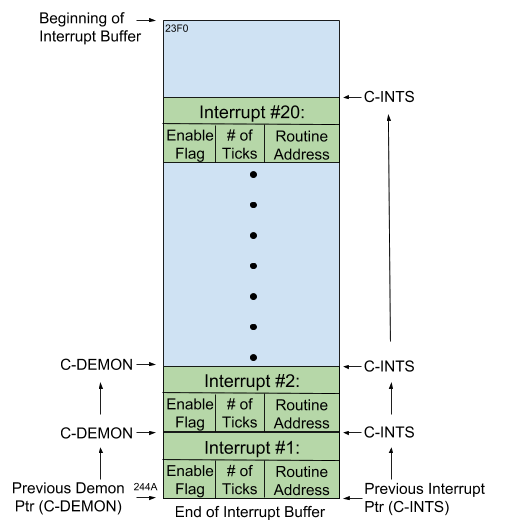
\includegraphics[width=0.8\textwidth]{figures/Interrupts}
\par\end{centering}
\caption{Interrupts}

\end{figure}


\subsection{QUEUE - Setting Up the Interrupts}
\begin{description}
\item [{Arguments:}] Routine address, Number of turns
\item [{Returns:}] Address of interrupt entry
\end{description}
With the first generation interrupt routines, QUEUE was a separate
routine to set the number of turns, or TICKS. It would call INT to
get the address to the interrupt entry for the request routine address
(creating the entry if necessary). Then. it would store the number
of ticks for that interrupt in the 2nd word value of that entry and
return the address to this interrupt entry. The setting of the enable
flag was not done and have to be done using a separate STORE command.
The last few ZIP 3 games (\textbf{Stationfall} and \textbf{The Lurking
Horror}) and most EZIP games (all except \textbf{AMFV}) and all XZIP
games did not use QUEUE. INT would automatically queue those entries
or the games would do it without a separate routine.

\subsection{CLOCKER - Running Interrupts}
\begin{description}
\item [{Arguments:}] None
\item [{Returns:}] TRUE if an interrupt was executed, FALSE if no interrupt
was executed
\end{description}
CLOCKER is the main routine that checks each interrupt entry and decreases
the number of turns for any enabled entry. It will call the routine
at the address stored in any interrupt entry with only 1 TICK left
or -1 TICKS which indicates the entry will always be executed. CLOCKER
is always called at the end of the MAIN-LOOP.
\begin{itemize}
\item If the given command was valid, CLOCKER will search through the interrupt
table for entries with their enable flag set and extract the number
of turns left.
\begin{itemize}
\item The search begins with the newest interrupt entry and proceeds to
the oldest entry.
\end{itemize}
\item If the TICKS is zero, CLOCKER goes to the next entry.
\item If the TICKS is not zero (a negative, 1, or greater than 1) then it
will be decreased by 1 and saved back into the entry.
\item If the TICKS is still greater than 1, then CLOCKER will then go to
the next entry.
\item At this point, CLOCKER will call the routine at the addr stored in
the interrupt entry. TICKS will be 1 or a negative number at this
point.
\end{itemize}
If no routine is called, CLOCKER will return FALSE. Otherwise, it
will return TRUE no matter how many routines are called. The actual
return value of the routine is not returned.

\subsection{What about DEMONs?}

INT allowed an initially set of interrupts to be added to the interrupt
table that are always checked regardless of the PARSER outcome. This
is marked by by the C-DEMONS pointer which moves from the end of the
interrupt table when new entries are created with the DEMON flag set.
C-INTS also moves when an entry is added when the DEMON flag is set.
In game design, these important interrupts are added first and end
up at the bottom of the interrupt table. All other interrupts but
be added above these entries. If PARSER fails on a given command,
CLOCKER will this and start checking the interrupts starting with
C-DEMON and not C-INT.

\textbf{Zork 1}\textquoteright s first use of these special, all-run,
interrupts were used for the demons and monsters in the game. This
term is very similar to \textquotedblleft daemons\textquotedblright{}
in operating systems where background processes can run on their own.
However, Infocom\textquoteright s use of the word \textquotedblleft demon\textquotedblright{}
came after \textquotedblleft daemon\textquotedblright{} was already
used by other programmers. It is probably just a happy coincidence.

\subsection{Update: New INT and Interrupt Entry}

All of the ZIP 1 and 2 games and most of the ZIP 3 games use the same
INT routine as seen in Zork 1. \textbf{Cutthroats}, \textbf{HGTG},
and \textbf{Suspect} used a slightly modified INT where DEMON pointer
is omitted. The first major change was with \textbf{AMFV} where the
size of the interrupt entry shrank to 2 words by removing the ENABLE
flag. Now, each entry with non-zero TICKS is considered enabled. Most
of the ZIP 3 games since \textbf{LGOP} also used this more compact
interrupt entry structure. \textbf{AMFV}\textquoteright s version
also kept track of the most recent blank entry which would be used
when storing a new entry instead of creating a new one. If new entry
needs to be created beyond the limits of the table, an error message
is displayed but the entry is still created.

\textbf{LGOP} also introduced a smarter INT routine that build off
the one from \textbf{AMFV}. It would \textquotedblleft remove\textquotedblright{}
any entries at the top of the table with no more TICKS left by moving
C-INT and skipping over these completed entries. Any entries with
no more TICKS surrounded by entries that were still enable were not
removed. This smarter INT also modified how interrupts during the
game initialization are stored. It would convert their TICK numbers
(by increasing it by 3 and making it negative) to label these interrupts
so they would not be called until CLOCKER had already been executed.
So, the first call of CLOCKER would convert these entries back to
normal entries (converting the TICKS back to positive values and subtracting
3) and then be checked on the next call to CLOCKER. So, these initial
interrupts would be bypassed at the start.

Only a few subsequent Infocom games modified their INT routines beyond
what was mentioned. A few added special flag checks that would quit
out of INT. \textbf{Borderzone} and \textbf{Sherlock} both used time
more than ticks and had modified INT routines to reflect that. 

\subsection{Update: New CLOCKER}

CLOCKER also went through multiple modifications over successive games.
The ZIP 2 version added the CLOCK-WAIT flag which skips checking any
interrupts (including DEMON ones) when set and is cleared. This feature
is only important for the WAIT command which already calls CLOCKER
3 times by default. Without this flag, the MAIN-LOOP will also call
CLOCKER after WAIT is completed. So there would be 4 calls to CLOCKER
for a WAIT command which is seen in ZIP 1. So the flag helps clear
up that confusion.

Some CLOCKER routines (like in \textbf{Deadline}, \textbf{Trinity},
\textbf{Bureaucracy}, \textbf{Borderzone}, and \textbf{Sherlock})
would also increment separate time variables (seconds, minutes, hours,
and possibly days) that the game would use for various situations.
These routines (like in \textbf{Deadline} and \textbf{Moonmist}) check
the number of turns or the elapsed time to see if the game should
end prematurely or reset specific counters. Others like Wishbringer
would check specific flags that would cause CLOCKER to execute routines
of specific entries if their TICK values were below a certain threshold.
Later versions (\textbf{Suspended}, \textbf{Infidel}, \textbf{Enchanter},
\textbf{Zork 1}, \textbf{Zork 2}, \textbf{Sorcerer}, \textbf{Moonmist},
\textbf{Ballyhoo}, \textbf{Mini-Zork}) increase the number of turns
in CLOCKER instead of MAIN-LOOP. \textbf{The Witness}, \textbf{Seastalker},
and \textbf{Cutthroats} return the first non-zero interrupt routine
result. However, if one of the routine returns M-FATAL, then that
will always be returned.

\textbf{Planetfall} corrected one logic error in the original INT
routine regarding entries with negative TICKS. Previously, any entry
with a negative TICK value would have its routine execute with the
TICK value decreasing as well. So subsequent calls to this entry would
make the TICK value more negative. Theoretically, that value could
then flip into the positive range because of the way negative numbers
are represented. Hexidecimal values of \$0001 to \$7FFF are positive
(1 to 32767) while \$8000 to \$FFFF are negative (-32768 to -1). If
a TICK value of \$8000 (-32768) is decreased by 1 again, the new value
\$7FFF now is 32767 and will not be executed on the next CLOCKER cycle.
\textbf{Planetfall} added a specific check for the \$FFFF (-1) TICK
value which would still execute the routine at the entry\textquoteright s
address but would not decrease the TICK value.

As mentioned before, \textbf{AMFV} uses the shortened 2 word entry.
Its CLOCKER also will clear out the routine address of any entry that
also has zero TICKS. This allows INT to use these blank entries for
new entries. \textbf{LGOP}\textquoteright s CLOCKER had the ability
to \textquotedblleft delete\textquotedblright{} entries that were
at the top of the interrupt table. It would lower the starting point
of the interrupt table to just past any blank or recently completed
entries. If any blank or completed entries were below a still enabled
entry, they could not be deleted. \textbf{Stationfall} and \textbf{Sherlock}
could decreased TICKS/time value by a different amount for all entries
with each call of CLOCKER. This allowed parts of the game to cause
interrupts to be executed soon than expected as each call of CLOCKER
will more rapidly drop the TICK counts.

\textbf{HGTG} still has the PARSER valid check to decide which pointer
to use. If the PARSER fails, the entire table is checked (\#00 as
pointer) instead of from the newest entry.

\subsection{Removing Interrupts with DEQUEUE}
\begin{description}
\item [{Arguments:}] Routine address
\item [{Return:}] TRUE if successful, FALSE if unable to find interrupt
\end{description}
DEQUEUE was introduced in LGOP and clears the routine address of the
entry with that address. Any dequeued entry would eventually be \textquotedblleft removed\textquotedblright{}
by CLOCKER.

\subsection{New Predicates for the Interrupts}

ENABLED?
\begin{description}
\item [{Arguments:}] Routine address
\item [{Return:}] TRUE if matching interrupt is enabled, FALSE if no match
found or interrupt is not enabled
\end{description}
RUNNING?
\begin{description}
\item [{Arguments:}] Routine address
\item [{Return:}] TRUE if matching interrupt has at least 1 TICK left,
FALSE if no TICKS left or no match found
\end{description}
Two new predicates were added, ENABLED? And RUNNING? in \textbf{Cutthroats}
to help find the status of specific interrupts. ENABLED? returned
TRUE if the ENABLED word in a matching interrupt entry was set. RUNNING?
returned TRUE if the TICKS in a matching entry was not zero, including
-1. In \textbf{LGOP}, ENABLED? was changed as no ENABLED word exists
in its entries. It would check the TICKS value and return TRUE if
it was non-zero including -1. \textbf{LGOP}\textquoteright s version
of RUNNING? would return TRUE if the matching entry\textquoteright s
TICK value was 1 or -1. So only entries that will be executed on the
next call of CLOCKER are considered running.

\section{Basic Screen Output and TELL}

\subsection{Introduction}

Infocom strived for readability, natural feel, and varied responses
of its games with its text routines. The games tried to be grammatically
correct with display articles before nouns and using plural forms
if necessary. Later games would fine tune these routines even more.
Infocom did use programming macros for creating the proper text display
routines. These macros would then be expanded into the proper ZIL
code during compiling. It is difficult to figure out which was the
first game to use this without the source code. The macros are seen
in the \textbf{Mini-Zork} source code.

\subsection{Abbreviations / Frequent words table}

Starting with ZIP version 2, Infocom games used abbreviations to help
reduce the space taken up by text. In version 2, the ZSCII character
\$01 signaled an abbreviation is to be display.The next ZSCII character
indicates the requested abbreviation. This allows for 32 abbreviations.
The abbreviation ZSCII character is consistent throughout the 3 character
sets. The previous new-line control character (ZSCII 1) was moved
to ZSCII 7 in character set 2.

To allow for more abbreviations, ZIP versions 3 and higher also use
characters \$02 and \$03 to signal an abbreviation. Since each of
these special control characters can access 32 abbreviations, these
games could have 96 abbreviation, calculated using the formation:
(abbreviation character value - 1) {*} 32 + next character\textquoteright s
ZSCII value. This also left only 2 control characters (ZSCII 4 and
5) remain to change the character set. Those control characters were
repurposed to change the character set for next character only. There
would be no \textquotedblleft shift lock\textquotedblright .

An abbreviation table contains 32 (or 96 for versions 3 or higher)
word addresses for the Z-strings. The abbreviation and next characters
will then point to an entry in this abbreviation table with an address
to a Z-string which will then be displayed. Because each abbreviation
uses 2 characters, abbreviations for string longer than 2 characters
could help reduce the size of the story file.

\subsection{Special PRINT Routines - WORD-PRINT, CLAUSE-PRINT, PREP-PRINT}

\textbf{Zork 1} also included three print routines that work with
the given command and prepositions:
\begin{itemize}
\item WORD-PRINT
\item PREP-PRINT
\item CLAUSE-PRINT
\end{itemize}
WORD-PRINT displays a sequence of characters from INBUF given the
starting character and number of characters to print.

PREP-PRINT displays the preposition given the preposition byte number,.
The routine uses PREP-FIND to convert the preposition byte number
to a Vocabulary address for the preposition. The only except is \textquotedblleft through\textquotedblright{}
which is larger than the 6 character limit for ZIP 3 or earlier. PREP-PRINT
looks for the corresponding preposition number and just display the
entire token.

CLAUSE-PRINT display the entire noun clause using the boundary addresses
stored in ITBL. A preceding preposition can also be displayed if the
preposition number is also passed as an argument. The boundary addresses
to use are based upon the element numbers in ITBL. Displaying the
token from Vocabulary or from INBUF depends on state of O-FLAG. The
routine will use strings from the Vocabulary (maximum of 6 characters)
if the O-FLAG is set. Otherwise, it will use WORD-PRINT to print the
entire token from INBUF. 

display the tokens in LEXV given by the start and end address of the
requested noun clause. This limited any token to 6 characters. If
the O-FLAG was clear, the routine extracted the length and location
of each token in INBUF and displayed the complete token.

\subsection{New versions PRINT routines}

Deadline introduced several 4 new routines and updated CLAUSE-PRINT
to improve the quality of the displayed text.

BUFFER-PRINT is a new routine that displays a sequence of tokens while
modifying any truncated or referred tokens. For example, the \textquotedblleft mrs\textquotedblright{}
token will then be displayed as \textquotedblleft mrs.\textquotedblright{}
while the \textquotedblleft it\textquotedblright{} token is replaced
with its referring object. The address of the starting token and token
after the last one to display are passed to the routine. The fourth
argument is a boolean value to indicate print a preceding space before
the first and subsequent tokens.

PRSO-PRINT and PRSI-PRINT are new routines that will display the direct
or indirect object clause, respectively. They extract the starting
and ending addresses of the clause from ITBL and see if the first
token in the clause is \textquotedblleft it\textquotedblright . If
so, the current PRSO is displayed. Otherwise, these addresses are
passed to BUFFER-PRINT.

The last new routine display a token with the first letter capitalized.
No official name is known but could be called CAPITALIZE-PRINT. The
routine pulls the first character and converts it to uppercase without
checking the case first. Then it will use WORD-PRINT to display the
remaining part of the token.

The new CLAUSE-PRINT utilizes BUFFER-PRINT to display those representative
tokens with their proper names. The routine will take the start and
end element numbers from ITBL and extracts the start and end addresses
for the tokens to print. These are then sent to BUFFER-PRINT.

Enchanter would later introduce THING-PRINT which takes a boolean
argument to choose which object clause to use (true for direct, false
for indirect). The routine pulls the start and end addresses for the
requested object clause and passes it to BUFFER-PRINT.

\subsection{Error message routines}

All Infocom games have several default error messages when handling
errors with given commands.
\begin{itemize}
\item CANT-USE
\item CANT-ORPHAN
\item UNKNOWN-WORD
\end{itemize}
CANT-USE was first used in \textbf{Deadline} and would insert an invalid
token into the phrase: The word \textquoteleft <word>\textquoteright{}
can\textquoteright t be used in that sense.

CANT-OPRHAN was added in Starcross and had the static message: That
command was incomplete. Why don't you try again?

UNKNOWN-WORD would display the word that is not found in Vocabulary:

\begin{lstlisting}[basicstyle={\ttfamily}]
[I don't know the word "<word>" in a way that I don't understand.]
\end{lstlisting}

and also updates the OOPS-TABLE with the location of the token that
is unrecognized.

\subsection{Using the TELL Macro}

Source code for Infocom games used macros where a specific keyword
and associated data would be replaced with code incorporating that
extra data. TELL was the universal way of displaying text. However,
this could result in repetitive code to display the same kind of text.
So, later design guides for Infocom games describes the use of the
TELL macro with multiple modifiers. But, the macros would not be replaced
with strings of ZIL code but a call to separate routines for displaying
text with any additional modifiers such as proper definite and indefinite
articles (depending on the type and number of the object) or ending
periods and linefeeds. \textquotedblleft Learning ZIL\textquotedblright{}
describes these modifiers. 

\section{The Describers - For Rooms and Objects}

\subsection{Introduction}

There are several routines in an Infocom games that specialize in
describing locations and objects which are an essential part of any
game. \textquotedblleft Learning ZIL\textquotedblright{} mentions
DESCRIBE-ROOM and DESCRIBE-OBJECTS, but there are also DESCRIBE-OBJECT,
PRINT-CONT, and later PRINT-CONTENTS which complete the needed routines
to display an object and its contents. For example, LOOK would call
DESCRIBE-ROOM and DESCRIBE-OBJECTS with the verbose argument set.
Other commands, like INVENTORY or LOOK-INSIDE, would call PRINT-CONT
on the WINNER or PRSO, respectively.

\subsection{PRINT-CONT}
\begin{description}
\item [{Arguments:}] Object or Room number, Verbose flag, LEVEL number
\item [{Returns:}] TRUE if there is some descriptive output, FALSE if none
given
\end{description}
PRINT-CONT will describe the contents of the objects contained in
the given object or room. The routine will first describe each object
by display the string in the FDESC (First DESCription) property of
the object. Any object that also can be seen inside (using SEE-INSIDE?
predicate) will have PRINT-CONT recursively called on it. If the routine
is being used to display the inventory of the WINNER\textquoteright s
possession, it will skip the display of the FDESC\textquoteright s
of all the objects. PRINT-CONT will then see if a special header (such
as \textquotedblleft You are carrying:\textquotedblright{} or \textquotedblleft The
<object> contains: \textquotedblleft ) needs to be displayed by seeing.
This is done when an inventory is requested or the objects have already
been \textquotedblleft touched\textquotedblright . This also needs
to be the first text displayed for that particular routine call. PRINT-CONT
will then call DESCRIBE-OBJECT on each object to have it described.
If any of these objects are an integral part of another object, then
PRINT-CONT is called recursively on this integral object to see if
anything else can be described. Once all the objects are checked again,
PRINT-CONT will also see if the WINNER is in a vehicle and if that
vehicle is part of the contents of the original requested object.
If so, then PRINT-CONT will be called on that vehicle. While a verbose
flag argument can be passed, it is never used. The LEVEL argument
determines the indent of the descriptive text uses spaces from the
IDENTS table (maximum of 5). As the routine does further recursion,
the level number increases along with the corresponding indent.

\subsection{DESCRIBE-OBJECT}
\begin{description}
\item [{Arguments:}] Object or Room number, Verbose flag, LEVEL number
\item [{Returns:}] TRUE if extra descriptive output given from internal
objects, FALSE if none given
\end{description}
DESCRIBE-OBJECT will try to display a descriptive text about an object
using the FDESC (if the object is untouched) or LDESC. If neither
is available, a generic description is given, \textquotedblleft There
is a\textquotedblright{} for level 0 or \textquotedblleft A\textquotedblright{}
for all other levels. If the WINNER is also in a vehicle, then a clarifying
\textquotedblleft (in the room)\textquotedblright{} is given to remind
the WINNER that the object is NOT in the vehicle. Also any objects
that have visible contents will be also called with PRINT-CONT to
display the contents of that object. Againa, the Verbose flag is not
used in the routine but passed to PRINT-CONT if it is called.

\subsection{DESCRIBE-OBJECTS}
\begin{description}
\item [{Arguments:}] Verbose flag
\item [{Returns:}] TRUE if there is some descriptive output, FALSE if none
given
\end{description}
DESCRIBE-OBJECTS will try to display a descriptive text for all the
objects in the current location (HERE). It will not display a description
of the location itself. If that location is not lit, the routine will
return with the error message \textquotedblleft I can\textquoteright t
see anything in the dark.\textquotedblright{} If any objects do exist
in the current location, DESCRIBE-OBJECTS will call PRINT-CONT with
this location and the current VERBOSE level if one is not given. Return
values are the same as PRINT-CONT.

\subsection{DESCRIBE-ROOM}
\begin{description}
\item [{Arguments:}] TRUE (if called by LOOK action)
\item [{Returns:}] TRUE if room description given, FALSE if too dark to
give description
\end{description}
DESCRIBE-ROOM will initially check if the room is dark, displaying
a too-dark error message if it is. The routine will then display the
room name and decide if a further descriptions should be given. If
it was not called by a LOOK command or SUPERBRIEF is SET, then no
further description is given. If the WINNER is in a vehicle which
is also in the room, the routine will indicate that with the clarifying
\textquotedblleft (You are in the <vehicle>.)\textquotedblright .
DESCRIBE-ROOM will then check if the Verbose flag is set, or the room
is untouched. Either situation would have the routine try to call
the room\textquoteright s ACTION routine with M-LOOK to provide a
description. If this fails, the room\textquoteright s LDESC string
will be used if possible. If a room is untouched, then that room\textquoteright s
TOUCHBIT will be set.

\subsection{PRINT-CONTENTS}
\begin{description}
\item [{Arguments:}] Object number
\item [{Returns:}] TRUE
\end{description}
PRINT-CONTENTS was added with \textbf{Sorcerer-R6} to quickly display
a list of objects in a room or container. The object names would be
separated by commas and \textquotedblleft and\textquotedblright ,
if necessary. If only one object was listed, then IT-OBJECT would
be updated with that object.

\subsection{Update: DESCRIBE-ROOM}

\textbf{Zork 2} added a new RARG (M-FLASH or \$04) on a room\textquoteright s
ACTION routine even if verbose is clear (minimal output). This allows
a room to display important information even if the room was already
touched or verbose is clear. It also added a final call to the WINNER\textquoteright s
vehicle\textquoteright s ACTION with M-LOOK (if in a vehicle) when
describing the current location.

\section{Common Routines and Predicates}

\subsection{Introduction}

Numerous routines are found in most or all Infocom games and provide
important functions that are not specific to a certain game or action.
Predicates are a special type of routines that return true or false
based upon the given arguments. \textquotedblleft Learning ZIL\textquotedblright{}
does give numerous examples. No systematic search has been made to
find all of these special routines found in all Infocom games. The
known ones can be divided into four main categories:
\begin{itemize}
\item Tables
\item Objects
\item Game States
\item Movements
\end{itemize}

\subsection{Table Routines and Predicates}

There are three common table routines used in Infocom games since
Zork 1:
\begin{itemize}
\item ZMEMQB (byte, address to table)
\item ZMEMQ (word, address to table, last element to check, first element
to check)
\item PICK-ONE (address to table)
\end{itemize}
ZMEMQB searches for a given byte in a table of bytes. The interested
byte and table are passed as arguments. After getting the number of
items in the table, the routine will step through each byte. If the
given byte is found, it returns true. Otherwise, it will return false.

ZMEMQ is similar to ZMEMQ but searches for a specific word in a table
of word up to the last element indicated. It also accepts one additional
argument: first element number to check. If this argument is not gien,
then it will use the beginning of the table. For example:

\begin{lstlisting}[basicstyle={\ttfamily}]
ZMEMQ(0x3EA0, TBL, 6, 2)
\end{lstlisting}

would search for the word 0x3EA0 in a table of words starting with
elements 2 through 6.

PICK-ONE, the original version, uses a table of words where one of
these elements is randomly picked and returned. The new PICK-ONE keeps
track of what elements have already been picked and will not pick
them again until all the others have been picked. This is accomplished
by \textquotedblleft sorting\textquotedblright{} the table of elements.
Any picked word is swapped with the first unpicked word. When only
0 unpicked words remain, the number of picked elements is reset which
causes the entire process to be repeated. It is quite ingenious.
\begin{enumerate}
\item Get total number entries (0th word) and number of previously picked
string address (1st word) of string address in the table
\item Decrease total number of entries by 1 as one of the entries is the
number of picked string addresses
\item Calculate the address of the first unpicked string address and number
of unpicked string addresses
\item Random pick a number with maximum number being the number of unpicked
string addresses
\item Get the string address at that random location
\item Swap that string address with the one located in the first original
unpicked string addresses group
\item Update the number of picked items (1st word in the table)
\item If all the items have been picked (number of picked items equal total
number of available address), then reset this value to zero.
\end{enumerate}
The picked word is then returned. Some games use both PICK-ONE returns
as different situations can demand different versions of the routine.

\subsection{Object Predicates}

As for the predicates, these will see if a given object can be interacted
with in specific ways.
\begin{itemize}
\item LIT?
\item HELD?
\item SEE-INSIDE?
\item ACCESSIBLE?
\item VISIBLE?
\item UNTOUCHABLE?
\item GLOBAL-IN?
\item TOUCHING? (not used)
\end{itemize}
LIT? is the main predicate in \textbf{Zork 1}. It checks if the WINNER
can see around in a given location by looking at the ONBIT attribute.
If the ONBIT is clear (location is dark), the routine will do a secondary
check if the given location is the same as the WINNER\textquoteright s
location. The secondary check will look for any objects in the given
location. If any are found, then the location is considered lit and
the routine will return TRUE.

HELD? is also in \textbf{Zork 1} and checks the location of the given
object\textquoteright s location. If it is not the WINNER, this location
replaces the given object and the routine loops back to get the new
location of the just found location. This continues until the location
is the WINNER (return TRUE) or the location of the object is blank
(return FALSE). Other versions such as in \textbf{Zork 3} uses a recursive
method to find the ultimate location of an object and also look for
the ROOMS and GLOBAL objects which result in a false response. \textbf{HGTG}
introduced a second argument which was a room or object. This would
be used instead of the WINNER to determine if the given object was
ultimately located in it. If no second argument was given, the routine
would check if the given object was inside the WINNER.

SEE-INSIDE? checks for specific attributes on a given object to see
if its contents are visible. This applies to containers such as a
box or a surface object like a table where objects can be placed on
it. The routine was first used with \textbf{Sorcerer} and checked
three attributes: INVISIBLE, OPEN, and TRANSPARENT. The contents of
an invisible object cannot be seen. An object that is open or transparent
can have its content seen from the outside. \textbf{Wishbringer} added
an initial check to see if the object is a surface which always leads
to a true response. If object was not a surface, open, or transparent,
the routine would check if the object is an Actor and not the WINNER.
Objects contained in an actor are always visible. \textbf{Hollywood
Hijinx} would check if the given object was a container. If it is
false, then the routine jumps to the section to check if the given
object is an Actor.

ACCESSIBLE? was first introduced in \textbf{Zork 3} and checks if
the given object can be used. There are objects that are visible but
cannot be used (an object inside a closed and transparent container).
It would return true if the given object was present in the current
location or is one of the game\textquoteright s GLOBAL objects.

VISIBLE? was also introduced in Sorcerer and sees if the given object
can be used or seen by the WINNER. The routine checks if the given
object is accessible using the ACCESSIBLE? predicate. If that is false,
the routine checks if the WINNER can see inside the given object\textquoteright s
location (for example if it is in a clear box) by using SEE-INSIDE?
If that is true, the routine will then recursively call VISIBLE? with
the object\textquoteright s location. Wishbringer used a slightly
different approach with checking to see if the object was invisible
first. If not, the location of the object is found with META-LOC (a
room or GLOBAL object). If it is on the WINNER, in the current room,
or a GLOBAL object, then it is considered visible. If the object is
located somewhere else, the routine calls ACCESSIBLE? to see if it
is accessible. If so, then consider it visible. Sherlock only uses
a single modified ACCESSIBLE? command that also calls a modified SEE-INSIDE?
routine. So this mimics the original form.

UNTOUCHABLE? is a curious predicate that seems to be only used in
\textbf{LGOP} to screen for various special situations where objects
are in the same room but cannot be touched. For example, an object
inside of inside of a cage that is also in the room with the WINNER
is considered untouchable. If the given object is in the current location,
held by the WINNER, or contained inside the WINNER, then it would
return FALSE (ie. it is touchable). 

GLOBAL-IN? is a simple predicate that takes two arguments, an object
and location, and checks if the object is a local-global for that
location. Essentially, the routine uses the ZMEMQB or SCAN\_TABLE
opcode to look for the given object in the GLOBAL property of the
location.

TOUCHING? is described in \textquotedblleft Learning ZIL\textquotedblright{}
as a predicate that takes an object and sees if it needs to be \textquotedblleft touched\textquotedblright{}
to perform the current action, PRSA. There is no evidence in any released
game of a separate predicate that performs this function. Many action
routines do a similar type of check, however.

\subsection{Object Routines}

The most common set of routines relate to objects. These include routines
and predicates. The routines return specific values:
\begin{itemize}
\item ROB
\item WEIGHT
\item META-LOC
\item FIND-IN
\end{itemize}
Another routine CCOUNT (container count) and REMOVE-CAREFULLY are
described in \textbf{Mini-Zork} too.

ROB moves all the objects from one location (room or container) to
another or empty destination. It will step through each object in
one location and insert into another (or null) and then move to the
next sibling object.

WEIGHT will add up the \textquotedblleft weights\textquotedblright{}
of all the objects in an object. This could be the PLAYER or a container.
The routine goes through each child object in the given object. If
the child object is a container, WEIGHT is called recursively on that
child object. For each object, the weight property is read and added
to the total for that object and returned. This routine is useful
to see if the PLAYER or container cannot hold any more objects. The
default weight for an object is set as one of the default property
values for the object table.

Starting with \textbf{Zork 1}, META-LOC would originally find the
room that an object is located. If the object was on the PLAYER or
non-existent, it would return false. \textbf{Starcross} used different
coding and also add defaulted to the \textquotedblleft Bridge\textquotedblright{}
for any non-attached object. The Witness expanded the return values
to also LOCAL-GLOBALS and GLOBALS objects.

FIND-IN will try to find an object in the given location with the
given flag number set. It will return the first object found. If no
object exists with that given flag set, FALSE is returned. \textquotedblleft Learning
ZIL\textquotedblright{} does mention that if more than one object
has the given flag set, FIND-IN would also return false. However,
there are no examples of a routine that keeps track of how many matches
were found. All routines will exit after finding that first match.
Some of the later games also except a string with the other arguments.
This string will be displayed with the matched object name.

Two other routines in \textbf{Mini-Zork} are not documented by \textquotedblleft Learning
ZIL\textquotedblright . CCOUNT will count the number of objects in
the given location. It will not count any objects inside containers.
REMOVE-CAREFULLY removes the given object unless \textquotedblleft it\textquotedblright{}
is given which clears out the IT-OBJECT variable. The routine then
calls NOW-DARK?.

\subsection{Game State Routines and Predicates}

Various routine will interact or change the different states in the
game such as if the player is dead or reset the status line.
\begin{itemize}
\item JIGS-UP (string)
\item INIT-STATUS-LINE (boolean ClearScreen?)
\item UPDATE-STATUS-LINE
\item NOW-DARK?
\item NOW-LIT?
\item VERB?
\item GAME-VERB?
\end{itemize}
JIGS-UP is in every game in some fashion. It is called when the PLAYER
is killed or the game is over. After the final score is displayed,
a string is passed to it wish is displayed along with all the possible
choices for the PLAYER to proceed such as restart the game or quit.
If the game is restarted, the opcode RESTART is executed which will
restart the interpreter and start execution with the GO routine.

The status line routines, INIT-STATUS-LINE and UPDATE-STATUS-LINE,
are described in \textquotedblleft Learning ZIL\textquotedblright as
a common routine, but only \textbf{Sherlock} seems to use it. Usually,
the status line updates are handled by the routine for the READ opcode
and is part of the Z-machine interpreter.

NOW-DARK? and NOW-LIT? are routines and not predicates. No arguments
are passed to them. LGOP appears to be the first game that used these.
However, there is little evidence that subsequent games incorporated
this routine. NOW-DARK? sees if the current location is lit. If so,
then it will clear the LIT global variable and provide a warning message.
NOW-LIT? is the exact opposite except it will also call the V-LOOK
routine after setting LIT.

VERB? is a predicate that returns TRUE if PRSA is equal to any of
the given verbs in the predicate arguments. This does not actually
call a routine but is expanded into a set of multiple commands based
upon how many verbs are given.

GAME-VERB? is a simple predicate that checks if the current PRSA is
one of the \textquotedblleft game verbs\textquotedblright{} or a verb
that does not trigger the CLOCKER routine. While \textquotedblleft Learning
ZIL\textquotedblright{} mentions a GAME-VERB list, it is unclear if
this is a global list in ZIL or hard coded into the routine.

\subsection{Movement Routines}

Since moving the PLAYER or actors is a very common action, Infocom
games use three common routines to perform it:
\begin{itemize}
\item GOTO (room number)
\item DO-WALK (direction)
\item OTHER-SIDE
\end{itemize}
GOTO essentially moves the user to the requested location while still
calling the destinations action routine with M-ENTER and getting a
description. It does not check if the actor or WINNER is able to directly
get to the location. Some people consider it like teleporting into
a location.

DO-WALK is similar to GOTO but it uses PERFORM which performs all
necessary checks (unlike GOTO). DO-WALK sets the direction of movement
(P-WALK-DIR) and calls the V-WALK using PERFORM with that DIR.

OTHER-SIDE is given an object number of a door and returns the room
number on the opposite side of the first door in the room. The routine
steps through all the exit properties (highest to lowest) of the given
room until it finds a door object (the property will be 5 bytes long).
It the door object for that property matches the given door object,
it will then return the room number associated with that exit.

\newpage{}

\section{Conclusion - The End}

The creativity in designing the original ZORK on PDP main frame computer
can be almost directly seen in the microprocessor version of all Infocom
games. The structuring of rooms and objects, storing grammatical information,
and the innovative parser led to a surprisingly complex and interactive
game that could fit on a floppy disk. The use of a virtual Z-machine
was the first known use of a virtualization in a home computer as
well. A present day interactive fiction creator can now design their
own games without having to start from scratch. But an ambitious programmer
today can now use these essential data structures and routines to
create their own fairly complex IF system if they want. While better
game engines with more powerful parser and complex games already exist,
the sophistication of these early text adventure games in just about
60K of memory is a testament to all of the programmers\textquoteright{}
skill with ZIL and the efficiency of Z-code. Hopefully, the information
here has helped cracked the inner workings of these legendary games
and made them more enjoyable and appreciated decades later.

\addsec{Appendix A: Story Headers}

\subsection*{Header Layout}

\subsubsection*{Original header layout found in all ZIP versions}

\begin{table}[H]
\begin{tabular}{|>{\raggedright}p{0.1\textwidth}|>{\raggedright}p{0.15\textwidth}|>{\raggedright}p{0.65\textwidth}|}
\hline 
Word No. & Name & Function\tabularnewline
\hline 
\hline 
00 & ZVERSION & Byte 0: Z-machine version

Byte 1: Z-machine mode\tablefootnote{Z-machine mode is described but never used (bit flags)}\tabularnewline
\hline 
01 & ZORKID & Release number\tabularnewline
\hline 
02 & ENDLOD & End address of pre-loaded memory (code and data),\linebreak{}
Base of High Memory (start of non-preloaded data)\tabularnewline
\hline 
03 & START  & Address of first instruction (not routine), Program Counter\tabularnewline
\hline 
04 & VOCAB & Address to Vocabulary table\tabularnewline
\hline 
05 & OBJECT & Object data address\tabularnewline
\hline 
06 & GLOBALS & Address to Global Variable table\tabularnewline
\hline 
07 & PURBOT & Start address of read-only (static) memory, code and data\tabularnewline
\hline 
08 & FLAGS & Flags, 16 bits\tabularnewline
\hline 
\end{tabular}
\end{table}


\subsubsection*{ZIP version 2 added the abbreviation information}

\begin{table}[H]
\begin{tabular}{|>{\raggedright}p{0.1\textwidth}|>{\raggedright}p{0.15\textwidth}|>{\raggedright}p{0.65\textwidth}|}
\hline 
09-0B & SERIAL & Bytes 12 to 17: Serial Number in ASCII characters (words also labeled
as SERIAL, SERI1, and SERI2)\tabularnewline
\hline 
0C & FWORDS & Address to Frequently used words (Abbreviation) table\tabularnewline
\hline 
\end{tabular}
\end{table}


\subsubsection*{ZIP version 3 added game information}

\begin{table}[H]
\begin{tabular}{|>{\raggedright}p{0.1\textwidth}|>{\raggedright}p{0.15\textwidth}|>{\raggedright}p{0.65\textwidth}|}
\hline 
0D & PLENTH & Length of game file (shifted??)\tabularnewline
\hline 
0E & PCHKSM & Checksum of game file\tabularnewline
\hline 
\end{tabular}
\end{table}


\subsubsection*{EZIP version extended story header layout}

\begin{table}[H]
\begin{tabular}{|>{\raggedright}p{0.1\textwidth}|>{\raggedright}p{0.15\textwidth}|>{\raggedright}p{0.65\textwidth}|}
\hline 
0F & INTWRD & Byte 1E: INTID/Interpreter number\linebreak{}
Byte 1F: INTVR/version\tabularnewline
\hline 
10 & SCRWRD\tablefootnote{This word is set by the ZIP at startup.} & Byte 20: SCRV, Screen size in lines (\$FF = printing terminal)\linebreak{}
Byte 21: SCRH, Screen width in characters \tabularnewline
\hline 
\end{tabular}
\end{table}


\subsubsection*{XZIP also extended story header layout}

\begin{table}[H]
\begin{tabular}{|>{\raggedright}p{0.1\textwidth}|>{\raggedright}p{0.15\textwidth}|>{\raggedright}p{0.65\textwidth}|}
\hline 
11 & HWRD & Screen horizontal size of display in pixels\tabularnewline
\hline 
12 & VWRD & Screen vertical size of display in pixels\tabularnewline
\hline 
13 & FWRD & Byte 26: Font height\linebreak{}
Byte 27: Font width\tabularnewline
\hline 
14 & LMRG & Screen left margin in pixels\tabularnewline
\hline 
15 & RMRG & Screen right margin in pixels\tabularnewline
\hline 
16 & CLRWRD & Byte 2C: Background color\linebreak{}
Byte 2D: Foreground color\tabularnewline
\hline 
17 & TCHARS & Pointer to table of terminating characters\tabularnewline
\hline 
18 & CRCNT & Counter for carriage returns\tabularnewline
\hline 
19 & CRFUNC & Function for carriage returns\tabularnewline
\hline 
1A & CHRSET & Pointer to character set table\tabularnewline
\hline 
1B & EXTAB & Pointer to extension table, if needed\tabularnewline
\hline 
1C-1F & USRNM & Bytes 38 to 3F: Username in ASCII characters\tabularnewline
\hline 
\end{tabular}
\end{table}


\subsection*{MODE Byte}

The MODE byte is the the second byte in the ZVERSION word of the story
header. No bits are used in the Zork 1 and 2 games released by Infocom.
Bits 0-1 are set by the ZAP assembler while bits 3 through 6 are set
by the ZIP on startup.

\subsubsection*{Mode bits for ZIP version 3}

\begin{table}[H]
\begin{tabular}{|>{\raggedright}p{0.1\textwidth}|>{\raggedright}p{0.3\textwidth}|>{\raggedright}p{0.5\textwidth}|}
\hline 
Bit No. & Bit Name & Function\tabularnewline
\hline 
\hline 
0 & byte-swap & 0 = high order byte first, 1 = low order byte first\tabularnewline
\hline 
1 & status line format & 0 = score/turns, 1 = hours:minutes\tabularnewline
\hline 
2 & machine-specific function & Story file split across two discs???\tabularnewline
\hline 
3 & Tandy bit & 0 = non-Tandy, 1 = Tandy (to censor some informatino)\tabularnewline
\hline 
4 & status line existence & 0 = present, 1 = hiding\tabularnewline
\hline 
5 & splitability & 0 = split screen functions ignored, 1 = split screen functions available\tabularnewline
\hline 
6 & reserved & Default font is a Variable-width font???\tabularnewline
\hline 
7 & reserved & ????\tabularnewline
\hline 
\end{tabular}
\end{table}


\subsubsection*{Mode bits for EZIP (ZIP version 4)}

\begin{table}[H]
\begin{tabular}{|>{\raggedright}p{0.1\textwidth}|>{\raggedright}p{0.3\textwidth}|>{\raggedright}p{0.5\textwidth}|}
\hline 
Bit No. & EZIP Bit Name & Function\tabularnewline
\hline 
\hline 
0 & ESPLIT (screen operations) & SPLIT/SCREEN/CLEAR functions\tabularnewline
\hline 
1 & EHINV (highlight inverse) & Inverse highlight is not available\tabularnewline
\hline 
2 & EHBLD (highlight bold) & Bold highlight is not available\tabularnewline
\hline 
3 & EHUND (highlight underline-italics) & Underline-italic highlight not available\tabularnewline
\hline 
4 & ECURS (cursor addressing) & CURSET/CURGET ignored\tabularnewline
\hline 
5 & ESOUN (SOUND opcode) & SOUND opcode is ignored\tabularnewline
\hline 
6 &  & Reserved\tabularnewline
\hline 
7 &  & Reserved\tabularnewline
\hline 
\end{tabular}
\end{table}

0 = not available/ignored, 1 = available

\subsubsection*{Mode bits for XZIP (ZIP version 5)}

\begin{table}[H]
\begin{tabular}{|>{\raggedright}p{0.1\textwidth}|>{\raggedright}p{0.3\textwidth}|>{\raggedright}p{0.5\textwidth}|}
\hline 
Bit No. & Bit Name & Function\tabularnewline
\hline 
\hline 
0 & XCOLOR & COLOR operations\tabularnewline
\hline 
1 & XDISP & DISPLAY (show images) operation\tabularnewline
\hline 
2 & XBOLD & Bold\tabularnewline
\hline 
3 & XUNDE & Italic/underline\tabularnewline
\hline 
4 & XMONO & Monospace style font\tabularnewline
\hline 
5 & XSOUN & SOUND\tabularnewline
\hline 
6 &  & Reserved\tabularnewline
\hline 
7 &  & Reserved\tabularnewline
\hline 
\end{tabular}
\end{table}

0 = not available/ignored, 1 = available

\subsubsection*{Extension table}

\begin{table}[H]
\begin{tabular}{|>{\raggedright}p{0.2\textwidth}|>{\raggedright}p{0.2\textwidth}|>{\raggedright}p{0.5\textwidth}|}
\hline 
MSLOCX & word 1 & \tabularnewline
\hline 
MSLOCY & word 2 & \tabularnewline
\hline 
MSETBL & word 3 & writable\tabularnewline
\hline 
MSEDIR & word 4 & writable\tabularnewline
\hline 
MSEINV & word 5 & writable\tabularnewline
\hline 
MSEVRB & word 6 & writable\tabularnewline
\hline 
MSEWRD & word 7 & writable\tabularnewline
\hline 
BUTTON & word 8 & writable\tabularnewline
\hline 
JOYSTICK & word 9 & writable\tabularnewline
\hline 
BSTAT & word 10 & writable\tabularnewline
\hline 
JSTAT & word 11 & writable\tabularnewline
\hline 
\end{tabular}
\end{table}


\subsection*{FLAGS Bits}

\subsubsection*{FLAGS bits for ZIP}

\begin{table}[H]
\begin{tabular}{|>{\raggedright}p{0.1\textwidth}|>{\raggedright}p{0.1\textwidth}|>{\raggedright}p{0.2\textwidth}|>{\raggedright}p{0.5\textwidth}|}
\hline 
Bit No. & Versions & Bit Name & Function\tabularnewline
\hline 
\hline 
0 & 1-5 & FSCRI & Interpreter currently transcripting\tabularnewline
\hline 
1 & 3-4 & FFIXE & Fixed-width font needed\tabularnewline
\hline 
2 & 4-5 & FSTAT & Refresh Status Line (by interpreter)\tabularnewline
\hline 
3 & 5 & FDISP & DISPLAY (show images) available\tabularnewline
\hline 
4 & 5 & FUNDO & UNDO available\tabularnewline
\hline 
5 & 5 & FMOUS & MOUSE available\tabularnewline
\hline 
6 & 5 & FCOLO & COLOR available\tabularnewline
\hline 
7-15 & 1-5 &  & Reserved\tabularnewline
\hline 
\end{tabular}
\end{table}

From E- and X-ZIP - Internal Infocom document

\addsec{Appendix B: Attributes and Properties From \textquotedblleft Learning
ZIL\textquotedblright{}}

\subsection*{Object Attributes (through YZIP)}
\begin{description}
\item [{TAKEBIT}] One of the most basic bits, this means that the player
can pick up and carry the object.
\item [{TRYTAKEBIT}] This bit tells the parser not to let the player implicitly
take an object
\end{description}
\begin{itemize}
\item This is important if the object has a value and must be scored, or
if the object has an NDESCBIT which must be cleared, or if you want
taking the object to set a flag or queue a routine, or...
\end{itemize}
\begin{description}
\item [{CONTBIT}] The object is a container; things can be put inside it,
it can be opened and closed, etc.
\item [{DOORBIT}] The object is a door and various routines, such as V-OPEN,
should treat it as such.
\item [{OPENBIT}] The object is a door or container, and is open.
\item [{SURFACEBIT}] The object is a surface, such as a table, desk, countertop,
etc.
\end{description}
\begin{itemize}
\item Any object with the surfacebit should also have the CONTBIT (since
you can put things on the surface) and the OPENBIT (since you can't
close a countertop as you can a box).
\end{itemize}
\begin{description}
\item [{LOCKEDBIT}] Tells routines like V-OPEN that an object or door is
locked and can't be opened without proper equipment.
\item [{WEARBIT}] The object can be wearable, not that it is actually being
worn.
\item [{WORNBIT}] This means that a wearable object is currently being
worn.
\item [{READBIT}] The object is readable. Any object with a TEXT property
should have the READBIT.
\item [{LIGHTBIT}] The object is capable of being turned on and off. Doesn't
mean that the object is actually on.
\item [{ONBIT}] For room, it is lit. Outdoor rooms should have ONBIT if
daytime. For objects, it is providing light. An object with the ONBIT
should also have the LIGHTBIT.
\item [{FLAMEBIT}] This means that the object is a source of fire.
\end{description}
\begin{itemize}
\item Object should also have the ONBIT and the LIGHTBIT
\end{itemize}
\begin{description}
\item [{BURNBIT}] The object is burnable.
\item [{TRANSBIT}] The object is transparent; objects inside it can be
seen even if it is closed.
\item [{NDESCBIT}] The object shouldn't be described by the describers.
\end{description}
\begin{itemize}
\item This usually means that someone else, such as the room description,
is describing the object. Any takeable object, once taken, should
have its NDESCBIT cleared.
\end{itemize}
\begin{description}
\item [{INVISIBLE}] Tells the parser not to find this object. The intention
is to clear the invisible at some point.
\item [{TOUCHBIT}] For rooms, player has been to the room at least once.
For objects, it has been taken or otherwise disturbed by the player
\end{description}
\begin{itemize}
\item Once the TOUCHBIT is set, if it has an FDESC, that FDESC will no longer
be used
\end{itemize}
\begin{description}
\item [{SEARCHBIT}] Tells the parser to look as deeply into a container
as it can in order to find the referenced object.
\end{description}
\begin{itemize}
\item Without the SEARCHBIT, the parser will only look down one level.
\item Objects with a SURFACEBIT essentially function as objets with a SEARCHBIT
\end{itemize}
\begin{description}
\item [{VEHBIT}] This means that the object is a vehicle, and can be entered
or boarded by the player.
\end{description}
\begin{itemize}
\item All objects with the VEHBIT should usually have the CONTBIT and the
OPENBIT.
\end{itemize}
\begin{description}
\item [{PERSONBIT}] This means that the object is a character in the game,
and such act accordingly.
\item [{FEMALEBIT}] The object is an ACTOR who is a female.
\item [{VOWELBIT}] Any verb default which prints an indefinite article
before the DESC, use \textquotedbl an\textquotedbl{} instead of \textquotedbl a.\textquotedbl{}
\item [{NARTICLEBIT}] The object's DESC doesn't not work with articles,
and they should be omitted.
\item [{PLURALBIT}] The object's DESC is a plural noun or noun phrase.
The DESC should act accordingly.
\item [{RLANDBIT}] Usually used for rooms, llets any routine know that
the room is dry land (as most are).
\item [{RWATERBIT}] The room is water rather than dry land
\item [{RAIRBIT}] The room is in mid-air, for those games with some type
of flying.
\item [{KLUDGEBIT}] This bit is used only in the syntax file.
\end{description}
\begin{itemize}
\item It is used for those syntaxes which want to be simply VERB PREPOSITION
with no object. Put (FIND KLUDGEBIT) after the object. The parser,
rather than complaining about the missing noun, will see the FIND
KLUDGEBIT and set the PRSO (or PRSI as the case may be) to the ROOMS
object.
\end{itemize}
\begin{description}
\item [{OUTSIDEBIT}] Used in rooms to classify the room as an outdoors
room.
\item [{INTEGRALBIT}] An integral part of another object, and can't be
independently taken or dropped.
\item [{PARTBIT}] The object is a body part: the HANDS object, for example.
\item [{NALLBIT}] This has something to do with telling a TAKE ALL not
to take something, but I don't recall how it works. Help???
\item [{DROPBIT}] Found in vehicles, this not-very-important flag means
that if the player drops something while in that vehicle, the object
should stay in the vehicle rather than falling to the floor of the
room itself.
\item [{INBIT}] Another not-too-important vehicle-related flag, it tells
various routines to say \textquotedbl in the vehicle\textquotedbl{}
rather than \textquotedbl on the vehicle\textquotedblright .
\end{description}

\subsection*{Object Properties (through YZIP)}
\begin{description}
\item [{NORTH,~SOUTH,~EAST,~WEST,~NE,~SE,~NW,~SW}] These are the
direction properties, generally used only in room definitions.
\end{description}
\begin{itemize}
\item Note that the cardinal direction properties are not abbreviated, but
that the non-cardinal ones are abbreviated. There is no direction
property called NORTHEAST, for example.
\end{itemize}
\begin{description}
\item [{UP,~DOWN}] These are just like the eight direction properties.
\item [{IN,~OUT}] These are just like the eight direction properties.
\end{description}
\begin{itemize}
\item If the player just types IN or OUT, this property will handle the
movement. Generally, it's a good idea to give the OUT property to
any room with only one exit.
\end{itemize}
\begin{description}
\item [{SYNONYM}] Contains a list of the nouns which can be used to refer
to the object.
\item [{ADJECTIVE}] Contains a list of the adjectives which can be used
to refer to the object.
\item [{ACTION}] Defines the action routine associated with the object.
\end{description}
\begin{itemize}
\item In the case of an object, the action routine is called when the object
is the PRSO or the PRSI of the player's input. In the case of a room,
the routine is called with M-BEG and MEND once each turn, with M-ENTER
whenever the room is entered, and with MLOOK whenever the describers
need to describe the room.
\end{itemize}
\begin{description}
\item [{DESCFCN}] Defines the routine which the describers use to describe
the object.
\end{description}
\begin{itemize}
\item This can be the same routine as the object's action routine, provided
that the routine is set up to handle the optional variable (M-OBJDESC
or M-OBJDESC?).
\end{itemize}
\begin{description}
\item [{CONTFCN}] Indicates a special ROUTINE to call for objects contained
in this object
\item [{GENERIC}] Defines the routine which handles cases where the parser
determines an ambiguity about which object the player is referring
to.
\end{description}
\begin{itemize}
\item In the absence of a generic property, the parser will simply ask \textquotedbl Which
FOO do you mean...\textquotedbl{}
\end{itemize}
\begin{description}
\item [{DESC}] Technically, this isn't a property, but it looks just like
one when you define an object.
\end{description}
\begin{itemize}
\item It contains the string which, in the case of objects,will be used
in verb defaults, player's inventory, etc. In the case of rooms, it
is the room name which appears before room description and on the
status line.
\end{itemize}
\begin{description}
\item [{SDESC}] Using this property is the only way to give an object a
changable DESC.
\end{description}
\begin{itemize}
\item You can't <PUTP .OBJECT ,P?DESC \textquotedbl new desc\textquotedbl >
but you can <PUTP .OBJECT ,P?SDESC \textquotedbl new desc\textquotedbl >.
Be warned, however, that if your game \textquotedbl shell\textquotedbl{}
isn't set up for SDESCs, you will have to change every verb default.
Also, be warned that doing this will increase the size of your game
by hundreds of bytes or more, since the verb defaults will no longer
simply TELL the desc of the object, but must instead call a little
routine which decides whether the object in question has an SDESC
or not.
\end{itemize}
\begin{description}
\item [{LDESC}] In the case of a room, this contains a string which the
describers use for the long description of the room.
\end{description}
\begin{itemize}
\item In the case of an object, this contains a string which the describers
use to describe the object if it is on the ground.
\end{itemize}
\begin{description}
\item [{FDESC}] This property, which isn't usually used in room definitions,
contains a string which the describers use to describe the object
before the first time it is moved.
\item [{LOC}] Once again, technically not a property, but it looks just
like one when you're creating an object.
\end{description}
\begin{itemize}
\item Simply, this property contains the name of the object which contains
this object (in the case of a room, this is the object ROOMS).
\end{itemize}
\begin{description}
\item [{SIZE}] Contains a number which is the size/weight of the object.
\end{description}
\begin{itemize}
\item Generally, it is only meaningful for a takeable object. If a takeable
object has no size property, the game usually gives it a default size
of 5. The size of an object affects the number of object that a player
can carry, how much of a container it takes up, and so on.
\end{itemize}
\begin{description}
\item [{CAPACITY}] Contains a number which is the capacity of the object.
\end{description}
\begin{itemize}
\item Generally, it is only meaningful for a container. If a container has
no size property, the game usually gives it a default capacity of
5. The capacity of a container affects the number of objects which
can be placed inside it.
\end{itemize}
\begin{description}
\item [{VALUE}] This property is used in many games that have scoring.
\end{description}
\begin{itemize}
\item The property contains a number; in the case of rooms, it is the number
of points the player gets for entering the room for the first time;
in the case of objects, it is the number of points the player gets
for picking up the object for the first time.
\end{itemize}
\begin{description}
\item [{GLOBAL}] Generally found only in room definitions, this property
contains a list of objects which are local-globals referencable in
that room.
\item [{OWNER}] Defines an object which is the owner of this object.
\end{description}
\begin{itemize}
\item For example, the SPORTS-CAR object might have the property (OWNER
CYBIL) so that the player could refer to the car as \textquotedbl Cybil's
car\textquotedbl{} even though Cybil isn't actually holding the car.
When Cybil sells the car to the player, you would <PUTP ,SPORTS-CAR
,P?OWNER ,PROTAGONIST> so that the player could now refer to it as
\textquotedbl my car.\textquotedbl{}
\end{itemize}
\begin{description}
\item [{TEXT}] This property contains a string which is used when the player
tries to read the object.
\end{description}
\begin{itemize}
\item It exists for those objects which would otherwise need an action routine
to handle READ but nothing else.
\end{itemize}
\begin{description}
\item [{THINGS}] Formerly known as the PSEUDO property, this property allows
you to create \textquotedbl pseudo-objects\textquotedbl{} with some
of the properties of real objects.
\end{description}
\begin{itemize}
\item They have three parts: a list of adjectives, a list of nouns, and
an action routine. Here's example: (THINGS (RED CARMINE) (SCARF ASCOT)
RED-SCARF-F). Pseudo objects are very limited, however. They cannot
have flags, and they cannot be moved. It is beneficial to use them
whenever feasible, because (unlike real objects) they take up no pre-load
space.
\end{itemize}
\begin{description}
\item [{ADJACENT}] Something to do with adjacent rooms and referencability.
Stu?
\item [{PLURAL}] Stu?
\item [{PICTURE}] Contains the name of a graphic from the picture file
associated with the room or object.
\item [{FLAGS}] This is another fellow which looks just like a property
but isn't actually a property.
\end{description}
\begin{itemize}
\item It contains a list of all the flags which are FSET in that object
at the start of the game. A list of the common flags can be found
in the next appendix. (BY the time YZIP was used, attributes were
just considered a list of flags in this property and not a special
entity).
\end{itemize}
For all exit (direction) properties, the type of exit depends on the
length of the property:
\begin{table}[H]
\begin{tabular}{|>{\raggedright}p{0.2\textwidth}|>{\raggedright}p{0.1\textwidth}|>{\raggedright}p{0.6\textwidth}|}
\hline 
Unconditional Exit & 1 byte & Byte 0: room number\tabularnewline
\hline 
No Exit & 2 bytes & Byte 0-1: Z-string address of exit error\tabularnewline
\hline 
Functional Exit & 3 bytes & Byte 0-1: Routine address, \linebreak{}
Byte 2: 00\tabularnewline
\hline 
Conditional Exit & 4 bytes & Byte 0: Room number, \linebreak{}
Byte 1: Global variable, \linebreak{}
Byte 2-3: Z-string address for exit error\tabularnewline
\hline 
Door Exit & 5 bytes & Byte 0: Room number, \linebreak{}
Byte 1: Door object number, \linebreak{}
Byte 2-3: Z-string address for exit error, \linebreak{}
Byte 4: 00\tabularnewline
\hline 
\end{tabular}
\end{table}

ZIL-course from the Infocom Cabinet does mention two attributes and
one property not mentioned in \textquotedblleft Learning ZIL\textquotedblright :
\begin{itemize}
\item FURNITURE attribute: The object is a piece of furniture that a player
or actor can sit on.
\item RMUNGBIT attribute: This applies to rooms only and indicates the room
does not exist or accessable. The appropriate error message needs
to be given in the LDESC property. This is a cleaner method of removing
a room.
\item IN property: The container of this object
\end{itemize}

\addsec{Appendix C: Object Attributes and Properties in Zork 1}

\subsection*{Attributes}

\begin{table}[H]
\begin{tabular}{|>{\raggedright}p{0.1\textwidth}|>{\raggedright}p{0.2\textwidth}|>{\raggedright}p{0.6\textwidth}|}
\hline 
\$00 & MAZEBIT & Room is part of the maze.\tabularnewline
\hline 
\$01 & HOUSEBIT & Room is part of the house.\tabularnewline
\hline 
\$02 & RLANDBIT & Room is on dry land.\tabularnewline
\hline 
\$03 & ONBIT & For objects, it gives light. For locations, it is lit. All outdoor
rooms should have ONBIT set.\tabularnewline
\hline 
\$04 & FLAMEBIT & Object can be a source of fire. LIGHTBIT should also be set.\tabularnewline
\hline 
\$05 & VEHBIT & Object can be entered or boarded by the player.\tabularnewline
\hline 
\$06 & LIGHTBIT & Object can be turned on or off.\tabularnewline
\hline 
\$07 & KNIFEBIT & Object can cut other objects.\tabularnewline
\hline 
\$08 & BURNBIT & Object can be burned.\tabularnewline
\hline 
\$09 & READBIT & Object can be read.\tabularnewline
\hline 
\$0A & SURFACEBIT & Object is a container and hold objects which are always visible. CONTBIT
and OPENBIT should be set as well.\tabularnewline
\hline 
\$0B & SWITCHBIT & Object can be turned on or off.\tabularnewline
\hline 
\$0C & TRYTAKEBIT & object could be picked up but other values or routines need to be
checked.\tabularnewline
\hline 
\$0D & OPENBIT & Object is can be opened or closed, refers to doors and containers.\tabularnewline
\hline 
\$0E & CONTBIT & Object is a container and can contain other objects or be open/closed/transparent.\tabularnewline
\hline 
\$0F & TRANSBIT & Object is transparent so objects inside it can be found even if OPENBIT
is clear.\tabularnewline
\hline 
\$10 & FOODBIT & Object can be eaten.\tabularnewline
\hline 
\$11 & TAKEBIT & Object can be picked up or carried\tabularnewline
\hline 
\$12 & ACCEPTBIT? & (can accept objects)\tabularnewline
\hline 
\$13 & SACREDBIT & \tabularnewline
\hline 
\$14 & PERSONBIT & Object is a character in the game.\tabularnewline
\hline 
\$15 & DOORBIT & Object is a door.\tabularnewline
\hline 
\$16 & DRINKBIT & Object can be drunk.\tabularnewline
\hline 
\$17 & TOOLBIT & Object can be used as a tool to open other things.\tabularnewline
\hline 
\$18 & CLIMBBIT & Object can be climbed\tabularnewline
\hline 
\$19 & INTEGRALBIT & Object cannot be taken separately from other objects, is part of another
object.\tabularnewline
\hline 
\$1A & INJUREDBIT & Object is injured but not dead.\tabularnewline
\hline 
\$1B & ALIVEBIT & Object is alive.\tabularnewline
\hline 
\$1C & TOUCHBIT & For object, it has been taken or used. For rooms, it has been visited.\tabularnewline
\hline 
\$1D & INVISIBLE & Object is not detected by the game.\tabularnewline
\hline 
\$1E & CANTENTERBIT & (or full of water bit)\tabularnewline
\hline 
\$1F & NONLANDBIT & Room is in or near the water.\tabularnewline
\hline 
\end{tabular}
\end{table}


\subsection*{Properties}

\begin{table}[H]
\begin{tabular}{|>{\raggedright}p{0.1\textwidth}|>{\raggedright}p{0.2\textwidth}|>{\raggedright}p{0.6\textwidth}|}
\hline 
\$01 & NOT USED & \tabularnewline
\hline 
\$02 & NOT USED & \tabularnewline
\hline 
\$03 & NOT USED & \tabularnewline
\hline 
\$04 & NOT USED & \tabularnewline
\hline 
\$05 & SPECIALOBJS & 0-2 entries of (dict addr, paddr for DESCFCN)\tabularnewline
\hline 
\$06 & LOCAL-GLOBALS & array of obj \#s that are valid to use with object\tabularnewline
\hline 
\$07 & BITCHECK & attribute \# to check???\tabularnewline
\hline 
\$08 & TEXT & address of z-string\tabularnewline
\hline 
\$09 & SIZE & weight or size of the object\tabularnewline
\hline 
\$0A & CAPACITY & maximum weight or size that on object can hold\tabularnewline
\hline 
\$0B & FDESC & addr to z-string of first description\tabularnewline
\hline 
\$0C & TREASUREVALUE & \tabularnewline
\hline 
\$0D & VALUE & pts scores when taking a prized obj or entering a secret room\tabularnewline
\hline 
\$0E & LDESC & addr to z-string of \textquotedbl lie on ground\textquotedbl{} description\tabularnewline
\hline 
\$0F & HEALTH & 0-5, 0 is healthy, 5 is dead\tabularnewline
\hline 
\$10 & ADJECTIVE & adjective value in byte\tabularnewline
\hline 
\$11 & ACTION & address to routine\tabularnewline
\hline 
\$12 & SYNONYM & vocabulary addresses of synonymous tokens (must have default name
too)\tabularnewline
\hline 
\$13 & LAND & exit\tabularnewline
\hline 
\$14 & OUT & exit\tabularnewline
\hline 
\$15 & IN & exit\tabularnewline
\hline 
\$16 & DOWN & exit\tabularnewline
\hline 
\$17 & UP & exit\tabularnewline
\hline 
\$18 & SW & exit\tabularnewline
\hline 
\$19 & SE & exit\tabularnewline
\hline 
\$1A & NW & exit\tabularnewline
\hline 
\$1B & NE & exit\tabularnewline
\hline 
\$1C & S & exit\tabularnewline
\hline 
\$1D & W & exit\tabularnewline
\hline 
\$1E & E & exit\tabularnewline
\hline 
\$1F & N & exit\tabularnewline
\hline 
\end{tabular}
\end{table}

\end{document}
